\documentclass[uplatex,a4paper,11pt,oneside,openany]{jsbook}

\usepackage[dvipdfmx]{graphicx}
\usepackage[dvipdfmx]{color}
\usepackage{amsmath,amssymb}
\usepackage{bm}
\usepackage{ascmac}
\usepackage{here}
\usepackage{url}
\usepackage{colortbl}
\usepackage{setspace}
\usepackage{multicol}
\usepackage{comment}

\setlength{\textwidth}{\fullwidth}
\setlength{\textheight}{40\baselineskip}
\addtolength{\textheight}{\topskip}
\setlength{\voffset}{-0.55in}

\begin{document}

\title{実習のための配布資料}
\author{s.matoike}
\date{\today}
\maketitle

\newpage

\chapter{トランジスタの静特性}

\section{実習の目的}

トランジスタの電極間の電圧や各電極に流れる電流を測定することによって、
電気的な特性を理解し、加えてその用途・役割について学習する。

\section{使用する機器}

\begin{itemize}
\item 回路計
\item トランジスタ(2SC1815-O、2SC1815-Y、2SC1815-GR)\footnote{except for BL}
\item 直流電流計2台(mA及び$\mu$A)
\item 直流電圧計2台
\item 直流安定化電源装置2台($V_{CC}$用と、$V_{BB}$用)
\end{itemize}

\section{実習}

実習する項目
\begin{enumerate}
\item[(1)] 実習装置について調べる
\item[(2)] $V_{CE}\;-\;I_C$特性(出力特性)を調べて、第1象限グラフを作成する
\item[(3)] $I_B\;-\;I_C$特性を調べて、第2象限グラフを作成する
\item[(4)] $V_{BE}\;-\;I_B$特性(入力特性)を調べて、第3象限グラフを作成する
\item[(5)] 直流負荷線について調べて、第1象限グラフに重ねて作図する
\end{enumerate}

\newpage

\subsection{実習装置について調べる}

実習装置の抵抗器(固定抵抗器2つ、半固定抵抗器1つ)の表示を記録して、
その抵抗器の公称値を調べる。また、回路計を使ってそれぞれの抵抗値を実測し、
公称値と比較する。

\begingroup
\renewcommand{\arraystretch}{1.4}
\begin{table}[H]
  \begin{center}
  \caption{装置の抵抗について調べる}%\label{tbl:t1}\vspace{2mm}
  \begin{tabular}{|c|l|c|wc{2cm}|wc{2cm}|wc{2cm}|} \hline
  項番 & \multicolumn{1}{c|}{項目} & カラーコード等の表示 & 公称値 & 実測値 \\ \hline
  1 & コレクタ側の固定抵抗器 & & & \\
  2 & ベース側の固定抵抗器 & & & \\
  3 & ベース側の半固定抵抗器 & & & \\ \hline 
  \end{tabular}
  \end{center}
\end{table}
\endgroup

\begin{figure}[H]
  \centering
   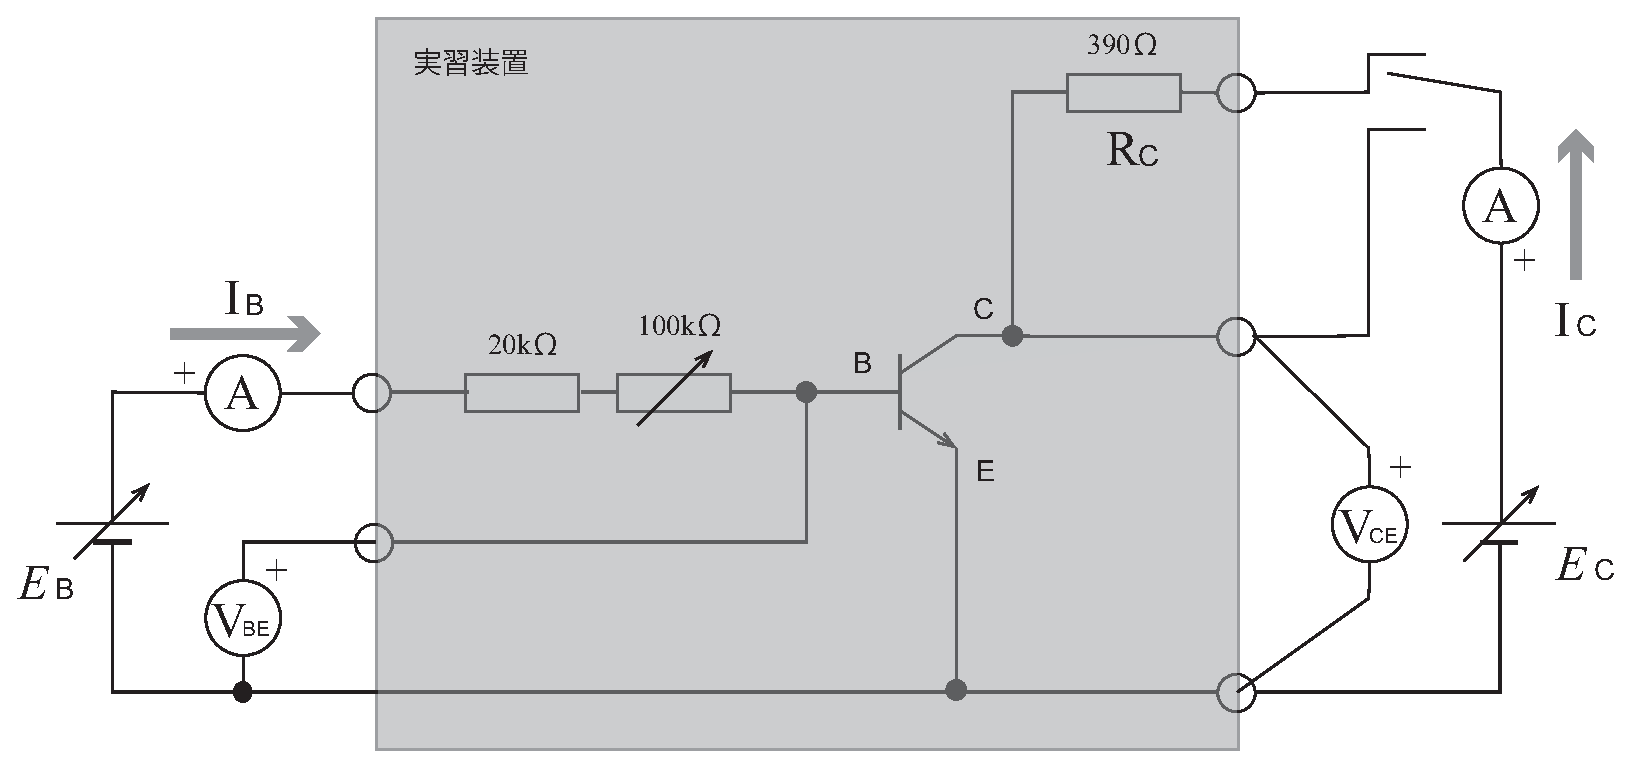
\includegraphics[keepaspectratio, scale=0.4, angle=0]
               {figs/eps/ex0.eps}
               \caption{実習装置}
               \label{fig:ex0}
\end{figure}

実習装置で使っているトランジスタの外観、及び名盤の表記をスケッチし、
トランジスタの図記号、端子の名称、各端子を流れる電流の呼称と表記、
端子間電圧の呼称と表記について調べて記録する。\\

\begin{comment}
	\begingroup
	\renewcommand{\arraystretch}{1.4}
	\begin{table}[H]
		\begin{center}
			\caption{トランジスタについて調べる(外観、端子、名称)}%\label{tbl:t1}\vspace{2mm}
			\begin{tabular}{|wl{6cm}|wl{6cm}|} \hline
				外観のスケッチ & トランジスタの名称\\
				& \\
				& 左の端子の名称\\
				& \\
				& 真ん中の端子の名称\\
				& \\
				& 右の端子の名称\\
				& \\ \hline
			\end{tabular}
		\end{center}
	\end{table}
	\endgroup
\end{comment}

\begin{figure}[H]
	\centering
	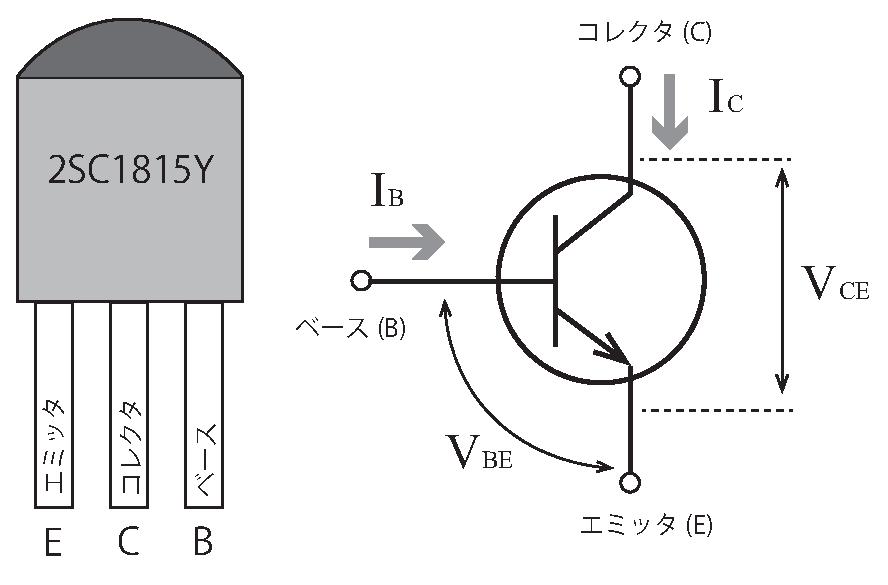
\includegraphics[keepaspectratio, scale=0.6, angle=0]
	{figs/eps/illust.eps}
	%\caption{}
	\label{fig:illust}
\end{figure}

\newpage

\subsection{出力特性:$V_{CE}\;-\;I_C$($I_B$一定):第1象限グラフ}

$V_{CE}-I_C$特性は出力特性とも呼ばれ、
ベース電流$I_B$一定の状態で、コレクタ-エミッタ間の電圧$V_{CE}$を変化させた時、
コレクタ電流$I_C$がどの様な変化をするかを示すもの。実験の手順は次の通り。
\begin{enumerate}
%\item[(1)] $V_{CE}=0.2$V にする(直流電源装置$E_C$を調節して)
\item[(1)] $V_{CE}=0.2$V、$I_B=20\;\mu$A に調節する(直流電源装置$E_C$、$E_B$、及び半固定抵抗器VRを操作)
%コレクタ電流$I_C$を測定し、記録する
%\item[(2)] $V_{CE}=0.2$Vに調整して、この時のコレクタ電流$I_C$を測定し、記録する
\item[(2)] $I_B=20;\mu$A のまま、$V_{CE}$を$0.4$〜$10.0$V に変えて、その都度$I_C$を測定して記録する
\item[(3)] $V_{CE}=0.2$V に戻し、$I_B$を$40,\;60,\;80\;\mu$A と変えて、それぞれの場合に上の手順2を実施する    
\end{enumerate}
横軸にコレクタ-エミッタ間の電圧$V_{CE}$、縦軸にコレクタ電流$I_C$をとって、第1象限のグラフを作図する

\vfill

\begin{figure}[H]
  \centering
   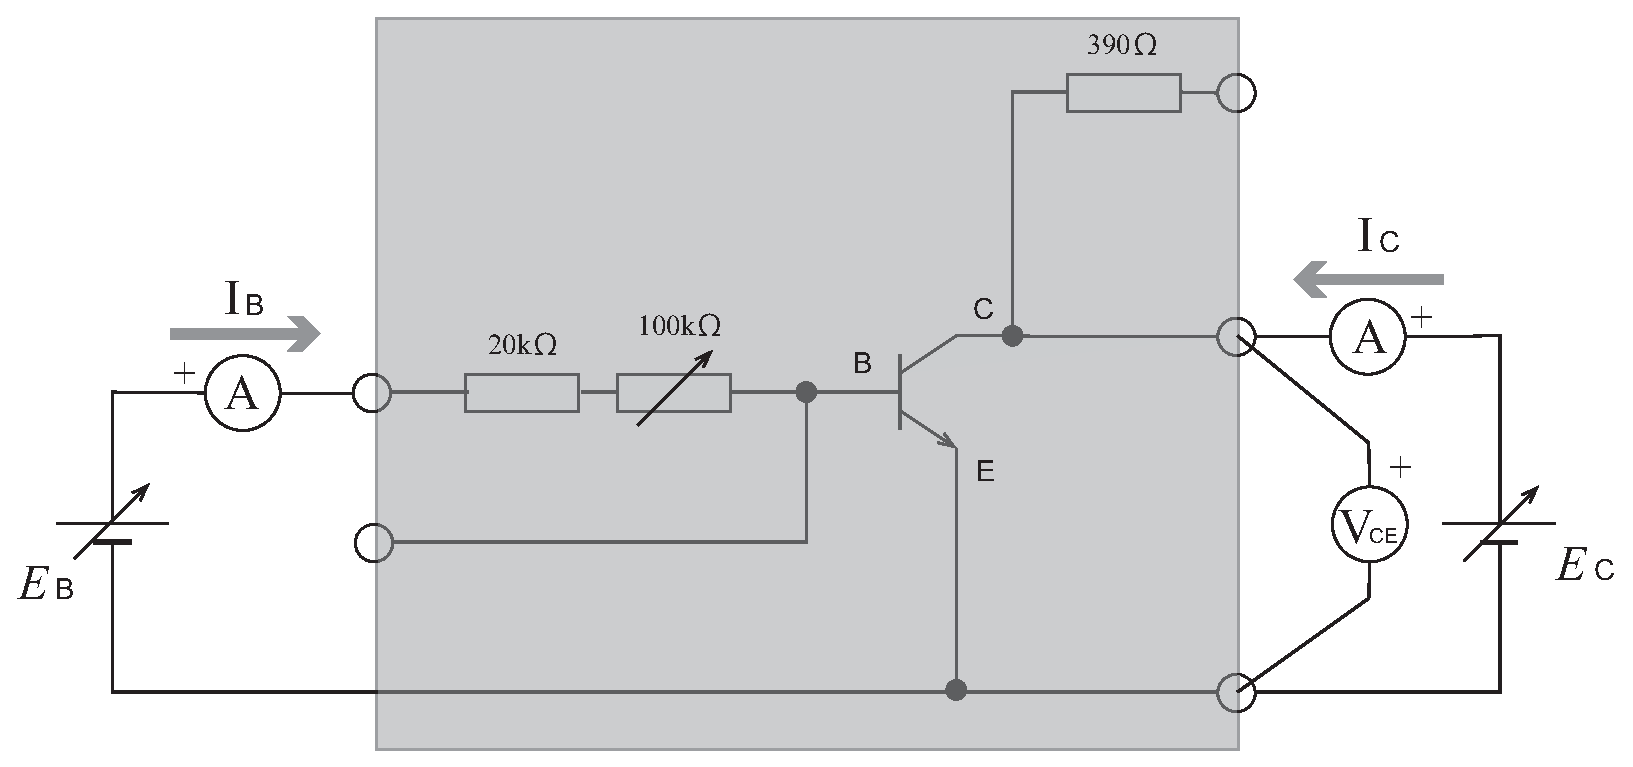
\includegraphics[keepaspectratio, scale=0.45, angle=0]
               {figs/eps/ex1.eps}
               \caption{出力特性$V_{CE}\;-\;I_C$($I_B$一定)}
               \label{fig:ex1}
\end{figure}

\vfill

\begingroup
\renewcommand{\arraystretch}{1.4}
\begin{table}[H]
  \begin{center}
  \caption{2SC1815:$V_{CE}\;-\;I_C$特性:$I_B$一定}%\label{tbl:t1}\vspace{2mm}
  \begin{tabular}{|r|wr{2.5cm}|wr{2.5cm}|wr{2.5cm}|wr{2.5cm}|} \hline
    \rowcolor[rgb]{0.9, 0.9, 0.9}
    &\multicolumn{4}{c|}{\textbf{コレクタ電流 $I_C$[mA] (2SC1815)}} \\ \hline
    \rowcolor[rgb]{0.9, 0.9, 0.9}
    \multicolumn{1}{|r|}{\textbf{$V_{CE}$[V]}} & \multicolumn{1}{c|}{\textbf{$I_B=20\mu$A}} & \multicolumn{1}{c|}{\textbf{$I_B=40\mu$A}} & \multicolumn{1}{c|}{\textbf{$I_B=60\mu$A}} & \multicolumn{1}{c|}{\textbf{$I_B=80\mu$A}} \\ \hline
    \multicolumn{1}{|r|}{\cellcolor[rgb]{0.9, 0.9, 0.9}\textbf{0.2}} & & & & \\ \hline
    \multicolumn{1}{|r|}{\cellcolor[rgb]{0.9, 0.9, 0.9}\textbf{0.4}} & & & & \\ \hline
    \multicolumn{1}{|r|}{\cellcolor[rgb]{0.9, 0.9, 0.9}\textbf{0.6}} & & & & \\ \hline
    \multicolumn{1}{|r|}{\cellcolor[rgb]{0.9, 0.9, 0.9}\textbf{0.8}} & & & & \\ \hline
    \multicolumn{1}{|r|}{\cellcolor[rgb]{0.9, 0.9, 0.9}\textbf{1.0}} & & & & \\ \hline
    \multicolumn{1}{|r|}{\cellcolor[rgb]{0.9, 0.9, 0.9}\textbf{2.0}} & & & & \\ \hline
    \multicolumn{1}{|r|}{\cellcolor[rgb]{0.9, 0.9, 0.9}\textbf{5.0}} & & & & \\ \hline
    \multicolumn{1}{|r|}{\cellcolor[rgb]{0.9, 0.9, 0.9}\textbf{8.0}} & & & & \\ \hline
    \multicolumn{1}{|r|}{\cellcolor[rgb]{0.9, 0.9, 0.9}\textbf{10.0}} & & & & \\ \hline
  \end{tabular}
  \end{center}
\end{table}
\endgroup

\newpage

\begin{figure}[H]
  \centering
   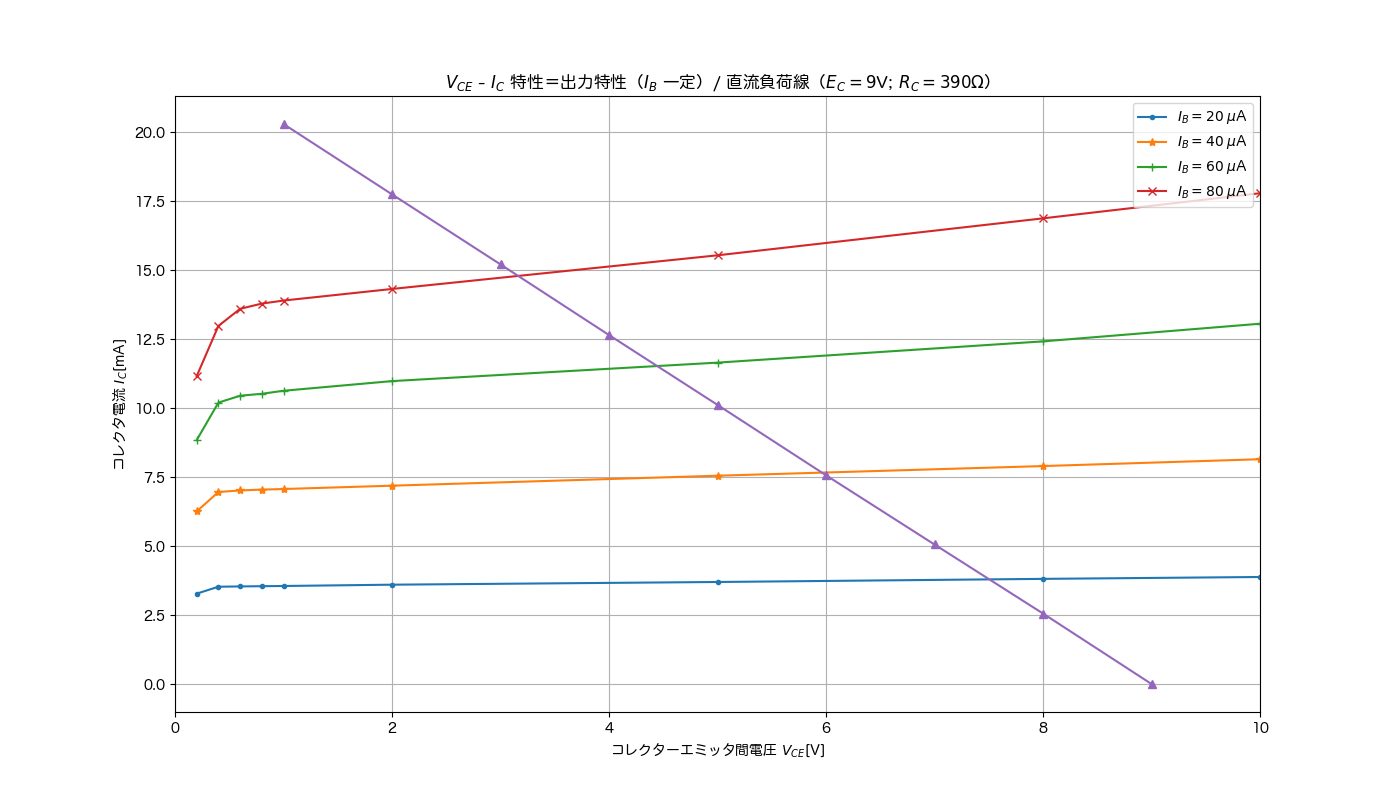
\includegraphics[keepaspectratio, scale=0.45, angle=0]
               {figs/png/x1static.png}
               \caption{グラフ作成例:出力特性及び直流負荷線(2SC1815Y)}
               \label{fig:iocharM1Yd}
\end{figure}

【結果の検討】

\begin{enumerate}
\item[(1)] $V_{CE}\;-\;I_C$特性のグラフより、$V_{CE}=5$V、$I_B=40\mu$A の時の$I_C$の値を読み取る\\
\item[(2)] この時の直流電流増幅率$h_{FE}=I_C/I_B$を求める\\
\item[(3)] このグラフから分かること(出力特性、$V_{CE}-I_C$特性)についてまとめる
\end{enumerate}

\newpage

\subsection{$I_B\;-\;I_C$特性($V_{CE}=5V$一定):第2象限グラフ}

$I_B\;-\;I_C$特性は、コレクタ-エミッタ間の電圧$V_{CE}$を一定にした状態で、
ベース電流$I_B$を変化させた時に、コレクタ電流$I_C$がどの様に変化するかを示すもの

この特性の傾き$I_C/I_B$は、直流電流増幅率$h_{FE}$と呼ばれる\\

実験の手順は次の通り

\begin{enumerate}
\item[(1)] $V_{CE}=5$V となるように$E_C$を調整し、測定中はこの値を維持する
\item[(2)] $E_B$(と必要に応じて可変抵抗器)を調整して、ベース電流$I_B$を$0$〜$80\;\mu$A まで$10\;\mu$A ずつ変化させ、
その都度コレクタ電流$I_C$を測定して記録する 
\end{enumerate}

測定を終えたら、横軸にベース電流$I_B$、縦軸にコレクタ電流$I_C$をとって、第2象限のグラフを作図し、
直流電流増幅率を求める

\vfill

\begin{figure}[H]
  \centering
   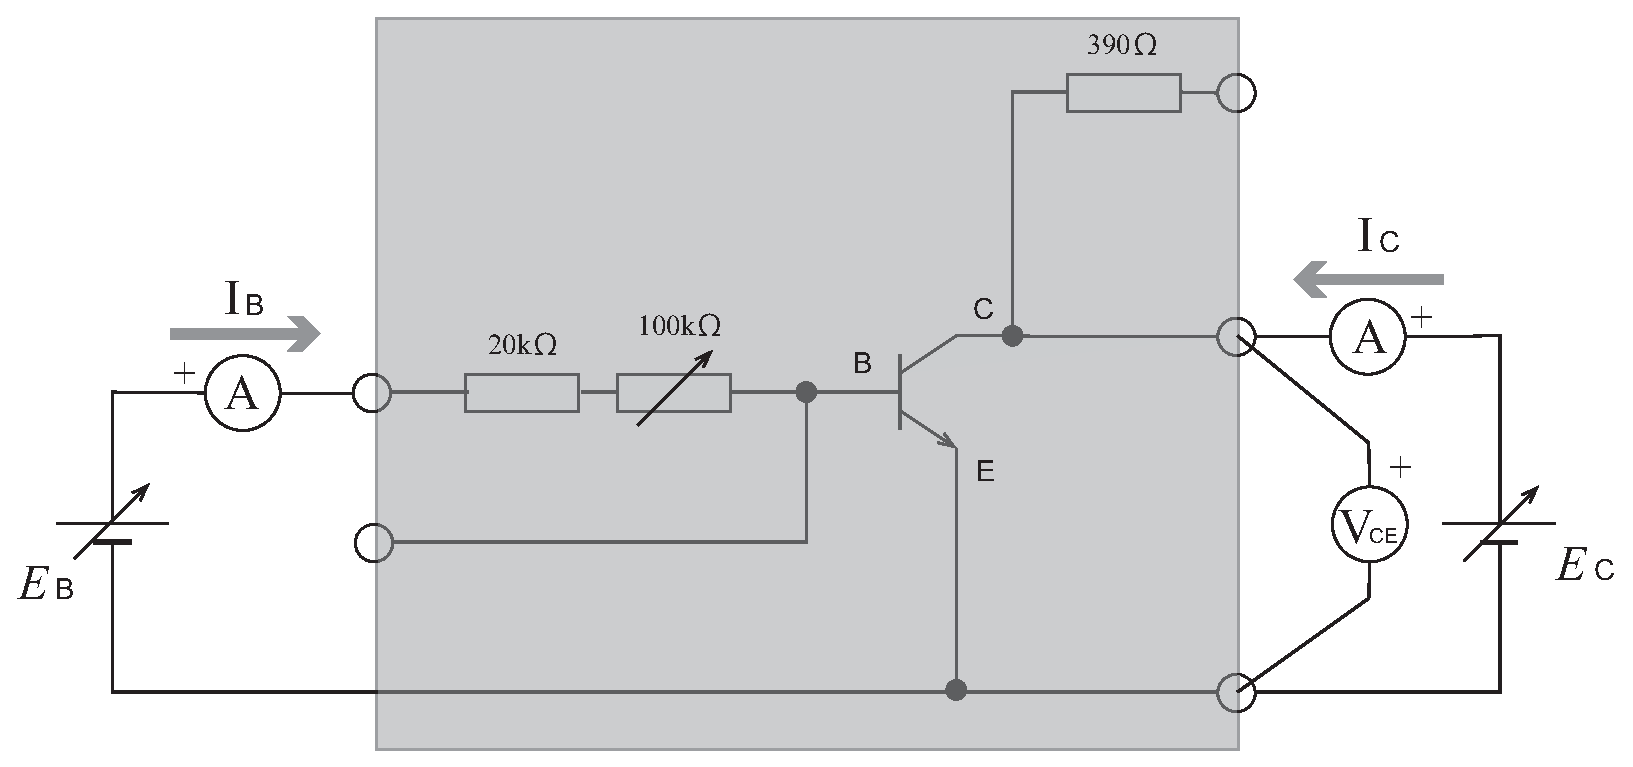
\includegraphics[keepaspectratio, scale=0.45, angle=0]
               {figs/eps/ex1.eps}
               \caption{$I_B\;-\;I_C$特性($V_{CE}=5$V 一定)}
               \label{fig:ex2}
\end{figure}

\vfill

\begingroup
\renewcommand{\arraystretch}{1.6}
\begin{table}[H]
  \begin{center}
  \caption{2SC1815:$I_{B}\;-\;I_C$特性:$V_{CE}=5$V一定}%\label{tbl:t5}\vspace{2mm}
  \begin{tabular}{|r|wr{1cm}|wr{1cm}|wr{1cm}|wr{1cm}|wr{1cm}|wr{1cm}|wr{1cm}|wr{1cm}|wr{1cm}|} \hline
    \rowcolor[rgb]{0.9, 0.9, 0.9}
    \multicolumn{1}{|r|}{\textbf{$I_B$[$\mu$A]}} & \multicolumn{1}{c|}{\textbf{0}} & \multicolumn{1}{c|}{\textbf{10}} & \multicolumn{1}{c|}{\textbf{20}} & \multicolumn{1}{c|}{\textbf{30}} & \multicolumn{1}{c|}{\textbf{40}} & \multicolumn{1}{c|}{\textbf{50}} & \multicolumn{1}{c|}{\textbf{60}} & \multicolumn{1}{c|}{\textbf{70}} & \multicolumn{1}{c|}{\textbf{80}}\\ \hline
    \multicolumn{1}{|r|}{\cellcolor[rgb]{0.9, 0.9, 0.9}\textbf{$I_C$[mA]}} & & & & & & & & & \\ \hline
  \end{tabular}
  \end{center}
\end{table}
\endgroup

\vfill

\newpage

\begin{figure}[H]
  \centering
   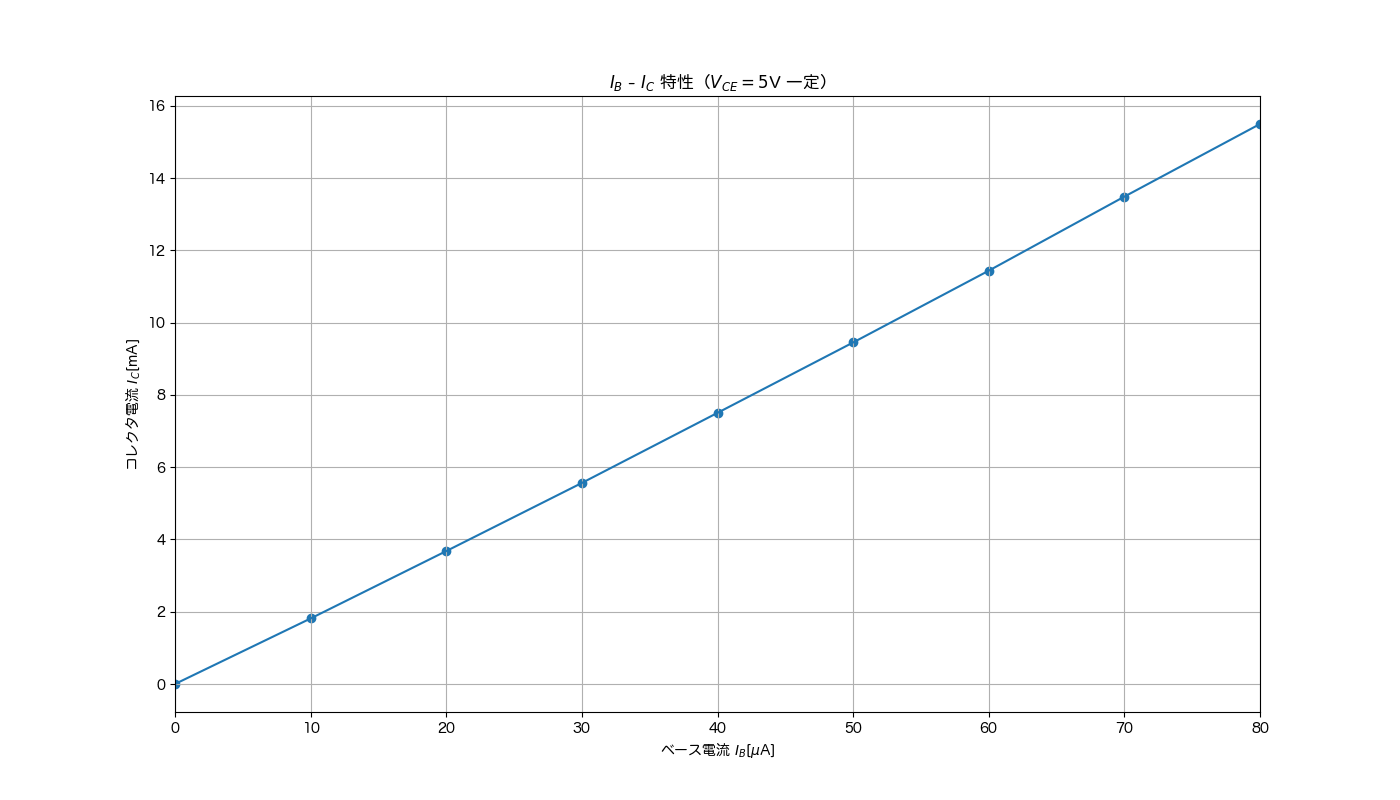
\includegraphics[keepaspectratio, scale=0.45, angle=0]
               {figs/png/x2static.png}
               \caption{グラフ作成例:$I_B\;-\;I_C$特性(2SC1815Y)}
               \label{fig:iocharM1Yd}
\end{figure}

【結果の検討】

\begin{enumerate}
\item[(1)] $I_B\;-\;I_C$特性のグラフより、$I_B=40\mu$A の時の$I_C$の値を読み取る\\
\item[(2)] この時の直流電流増幅率$h_{FE}=I_C/I_B$を求める\\
\item[(3)] $I_B=40\mu$A、$V_{CE}=5$V の点から、$I_B$を+方向に$20\mu$A だけ変化させた時の$I_C$の値をグラフから読み取る\\
\item[(4)] この時読み取った$I_C$の変化量から、この時の電流増幅率$h_{fe}=\Delta I_C/\Delta I_B$を求める\\
\item[(5)] このグラフから分かること($I_B-I_C$特性)についてまとめる
\end{enumerate}

\newpage

\subsection{入力特性$V_{BE}\;-\;I_B$($V_{CE}=5V$一定):第3象限グラフ}

$V_{BE}\;-\;I_B$特性は入力特性とも呼ばれ、コレクタ-エミッタ間の電圧$V_{CE}$を一定にした状態で、
ベース-エミッタ間の電圧$V_{BE}$を変化させた時、ベース電流$I_B$がどの様に変わるかを示すもの

この特性は、ダイオードの順方向特性とほぼ同じになる\\

実験の手順は次の通り

\begin{enumerate}
\item[(1)] $V_{CC}=5$V となる様に$E_C$を調整し、測定中はこの値を維持する
\item[(2)] $E_B$(必要に応じて可変抵抗器)を調整して、ベース-エミッタ間の電圧$V_{BE}$を変化させ、その都度ベース電流$I_B$を測定し記録する
\end{enumerate}

測定を終えたら、横軸にベース電流を、縦軸にベースエミッタ間の電圧をとって、
第3象限のグラフを作図する

\vfill

\begin{figure}[H]
  \centering
   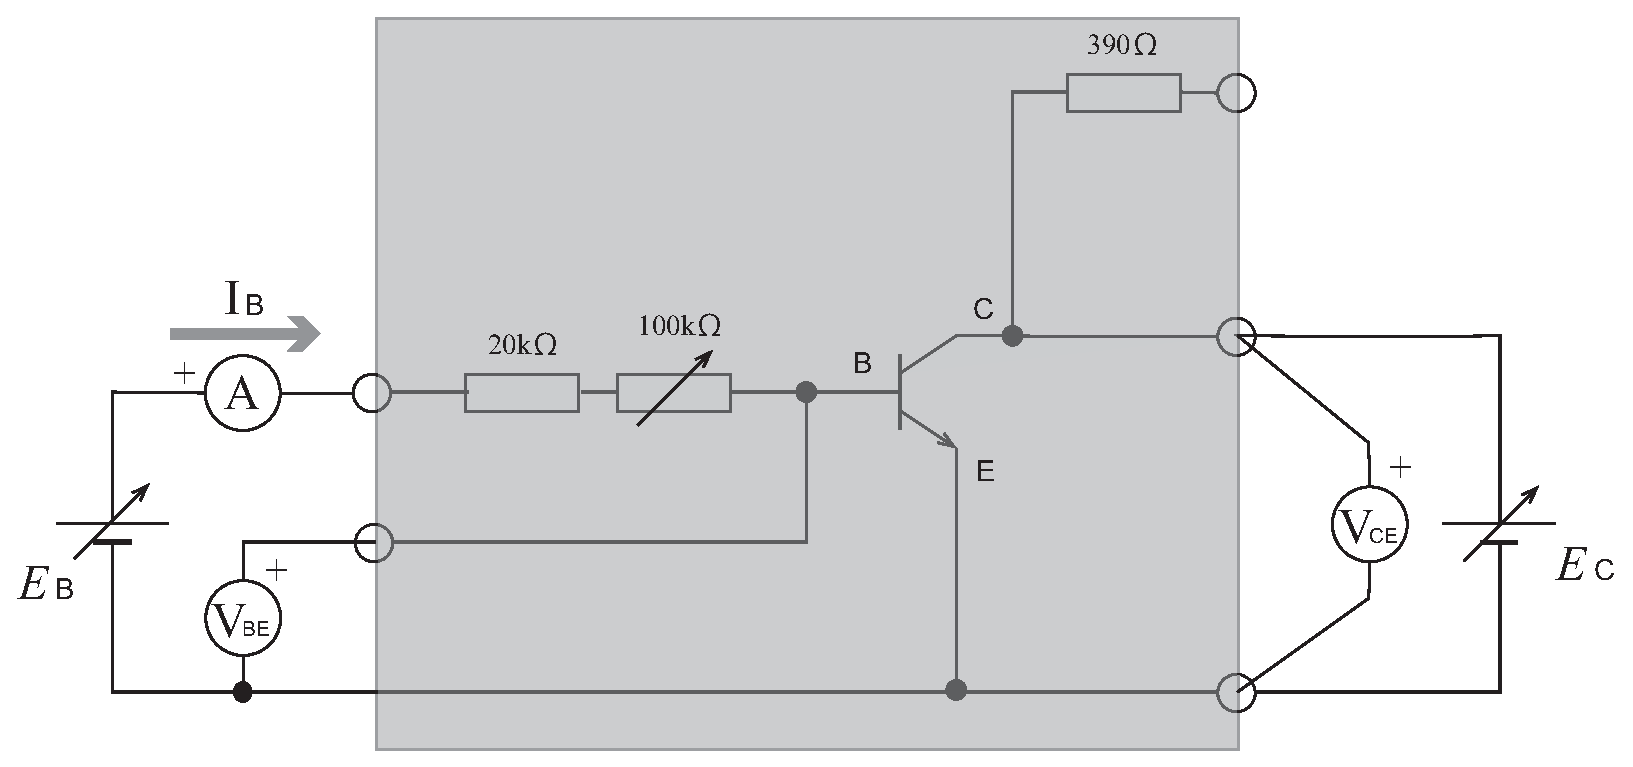
\includegraphics[keepaspectratio, scale=0.45, angle=0]
               {figs/eps/ex3.eps}
               \caption{入力特性$V_{BE}\;-\;I_B$($V_{CE}=5$V 一定)}
               \label{fig:ex3}
\end{figure}

\vfill

\begingroup
\renewcommand{\arraystretch}{1.6}
\begin{table}[H]
  \begin{center}
  \caption{2SC1815:$V_{BE}\;-\;I_B$特性:$V_{CE}=5$V一定}%\label{tbl:t9}\vspace{2mm}
  \begin{tabular}{|r|wr{1cm}|wr{1cm}|wr{1cm}|wr{1cm}|wr{1cm}|wr{1cm}|wr{1cm}|wr{1cm}|wr{1cm}|} \hline
    \multicolumn{1}{|r|}{\cellcolor[rgb]{0.9, 0.9, 0.9}\textbf{$V_{BE}$[V]}} & \multicolumn{1}{c|}{\cellcolor[rgb]{0.9, 0.9, 0.9}\textbf{0.2}} & \multicolumn{1}{c|}{\cellcolor[rgb]{0.9, 0.9, 0.9}\textbf{0.3}} & \multicolumn{1}{c|}{\cellcolor[rgb]{0.9, 0.9, 0.9}\textbf{0.4}} & \multicolumn{1}{c|}{\cellcolor[rgb]{0.9, 0.9, 0.9}\textbf{0.5}} & \multicolumn{1}{c|}{\cellcolor[rgb]{0.9, 0.9, 0.9}\textbf{0.6}} & & & & \\ \hline
    \multicolumn{1}{|r|}{\cellcolor[rgb]{0.9, 0.9, 0.9}\textbf{$I_B$[$\mu$A]}} & & & & & & \multicolumn{1}{c|}{\cellcolor[rgb]{0.9, 0.9, 0.9}\textbf{10.0}} & \multicolumn{1}{c|}{\cellcolor[rgb]{0.9, 0.9, 0.9}\textbf{20.0}} & \multicolumn{1}{c|}{\cellcolor[rgb]{0.9, 0.9, 0.9}\textbf{50.0}} & \multicolumn{1}{c|}{\cellcolor[rgb]{0.9, 0.9, 0.9}\textbf{80.0}}\\ \hline
  \end{tabular}
  \end{center}
\end{table}
\endgroup

\vfill

\newpage

\begin{figure}[H]
  \centering
   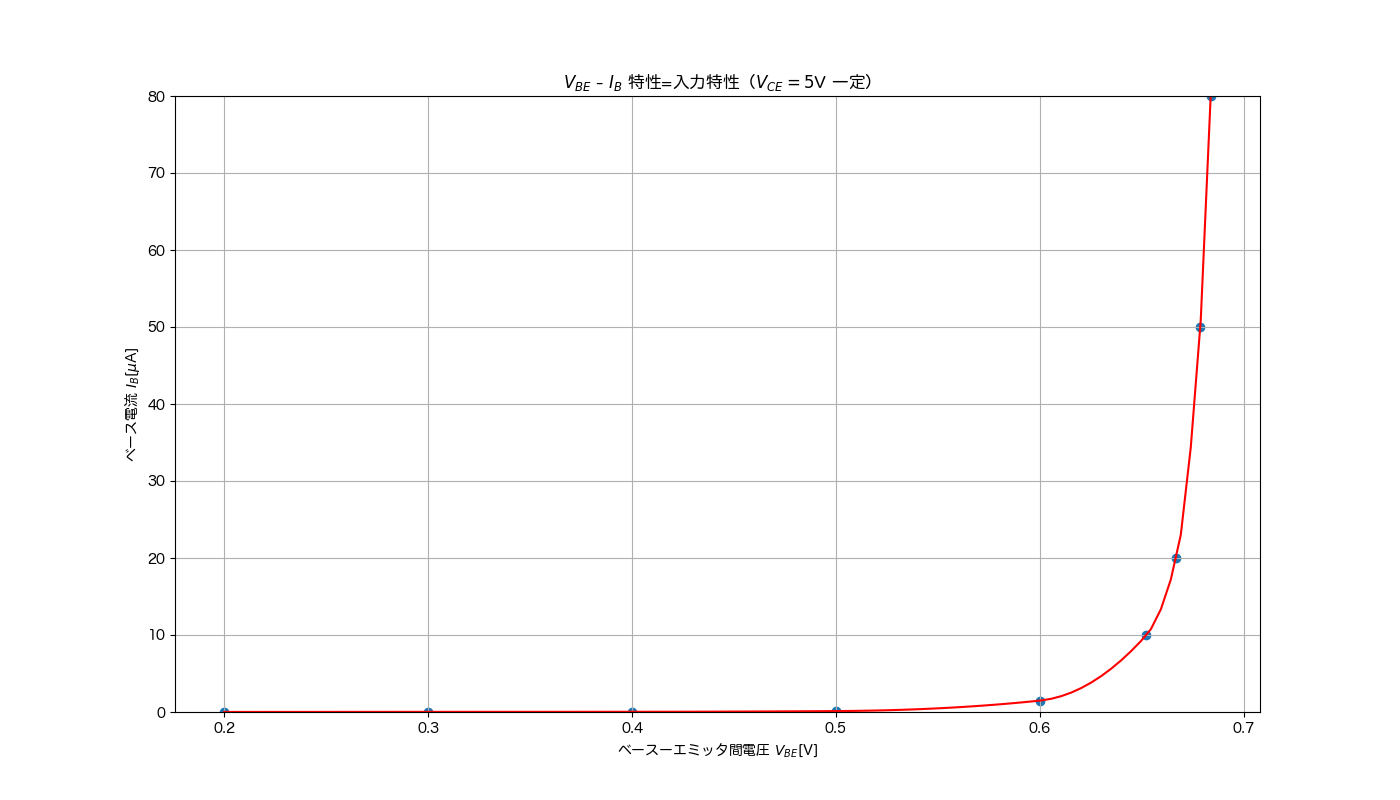
\includegraphics[keepaspectratio, scale=0.45, angle=0]
               {figs/png/x3static.png}
               \caption{グラフ作成例:入力特性(2SC1815Y)}
               \label{fig:iocharM1Yd}
\end{figure}

【結果の検討】

\begin{enumerate}
	\item[(1)] このグラフから分かること(入力特性、$V_{BE}-I_B$特性)についてまとめる
\end{enumerate}

\newpage

\subsection{直流負荷線($E_C=9V,\;R_C=390\Omega$):第1象限グラフ}

直流負荷線は、トランジスタのコレクタに負荷抵抗$R_C$が接続されている時の、
コレクタ-エミッタ間の電圧$V_{CE}$とコレクタ電流$I_C$の関係を示している

%コレクタ電流$I_C$の増加に伴い、コレクタ-エミッタ間の電圧$V_{CE}$は低下する\\

負荷抵抗$R_C=390\Omega$を通したコレクタ電流$I_C$を測定できる様に接続を変更した後、
次の手順で実験を進める

\begin{enumerate}
\item[(1)] ベース電流$I_B=0\;\mu$A になる様に$E_B$を調整し、その状態でコレクタ-エミッタ間の電圧$V_{CE}=9$V となる様に$E_C$を調整する(これ以降$E_C$には触らない)
\item[(2)] コレクタ-エミッタ間の電圧$V_{CE}$を観察しながら、$E_B$(必要に応じて可変抵抗器)を調整して$V_{CE}$を表\ref{tbl:tbl9}の通り変化させ、その都度コレクタ電流$I_C$測定して記録する  
\end{enumerate}

%測定を終えたら、第1象限に直流負荷線を作図する

%\vfill

\begin{figure}[H]
  \centering
   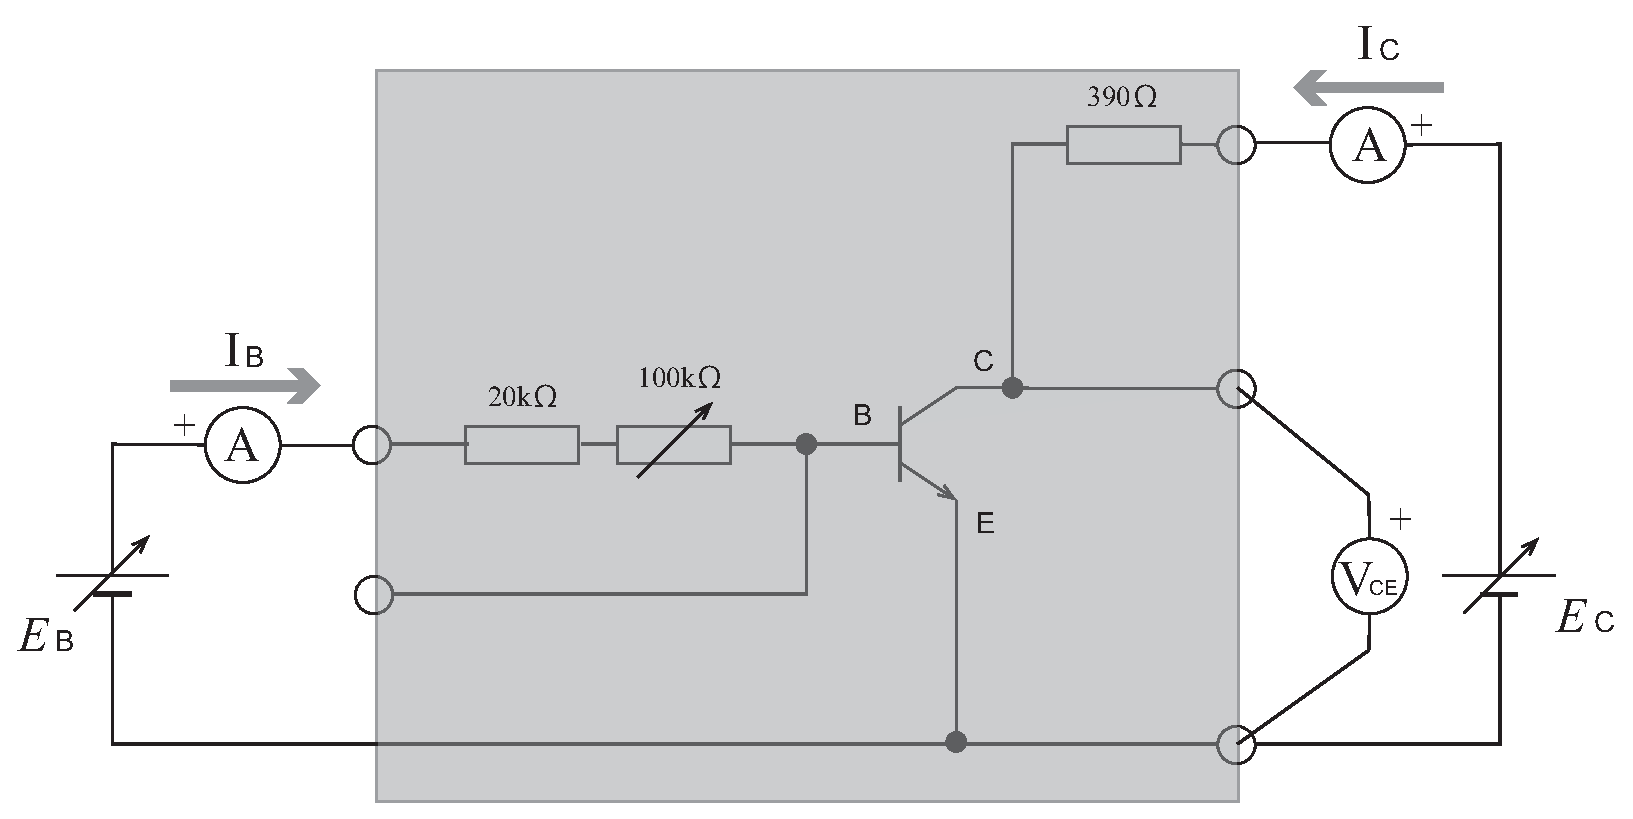
\includegraphics[keepaspectratio, scale=0.45, angle=0]
               {figs/eps/ex4.eps}
               \caption{直流負荷線}
               \label{fig:ex3}
\end{figure}

%\vfill

\begingroup
\renewcommand{\arraystretch}{1.6}
\begin{table}[H]
  \begin{center}
  \caption{2SC1815:直流負荷線:$E_{C}=9$V、$R_C=390\Omega$}\label{tbl:tbl9}\vspace{2mm}
  \begin{tabular}{|r|wr{1cm}|wr{1cm}|wr{1cm}|wr{1cm}|wr{1cm}|wr{1cm}|wr{1cm}|wr{1cm}|wr{1cm}|} \hline
    \multicolumn{1}{|r|}{\cellcolor[rgb]{0.9, 0.9, 0.9}\textbf{$V_{CE}$[V]}} & \multicolumn{1}{c|}{\cellcolor[rgb]{0.9, 0.9, 0.9}\textbf{9.0}} & \multicolumn{1}{c|}{\cellcolor[rgb]{0.9, 0.9, 0.9}\textbf{8.0}} & \multicolumn{1}{c|}{\cellcolor[rgb]{0.9, 0.9, 0.9}\textbf{7.0}} & \multicolumn{1}{c|}{\cellcolor[rgb]{0.9, 0.9, 0.9}\textbf{6.0}} & \multicolumn{1}{c|}{\cellcolor[rgb]{0.9, 0.9, 0.9}\textbf{5.0}} & \multicolumn{1}{c|}{\cellcolor[rgb]{0.9, 0.9, 0.9}\textbf{4.0}} & \multicolumn{1}{c|}{\cellcolor[rgb]{0.9, 0.9, 0.9}\textbf{3.0}} & \multicolumn{1}{c|}{\cellcolor[rgb]{0.9, 0.9, 0.9}\textbf{2.0}} & \multicolumn{1}{c|}{\cellcolor[rgb]{0.9, 0.9, 0.9}\textbf{1.0}}\\ \hline
    \multicolumn{1}{|r|}{\cellcolor[rgb]{0.9, 0.9, 0.9}\textbf{$I_C$[mA]}} & & & & & & & & & \\ \hline
  \end{tabular}
  \end{center}
\end{table}
\endgroup

%\vfill

直流負荷線のグラフは、第1象限の出力特性グラフに重ねて作図する。\\

%\vfill

【結果の検討】

\begin{enumerate}
\item[(1)] 直流負荷線を2等分する点の$V_{CE}$と$I_C$をグラフから読み取る\\
\item[(2)] 読み取った点の印をグラフ上に書き込む\\
\item[(3)] このグラフから分かること(直流負荷線、$V_{CE}-I_C$特性)についてまとめる
\end{enumerate}

%\vfill
\newpage

\begin{figure}[H]
  \centering
   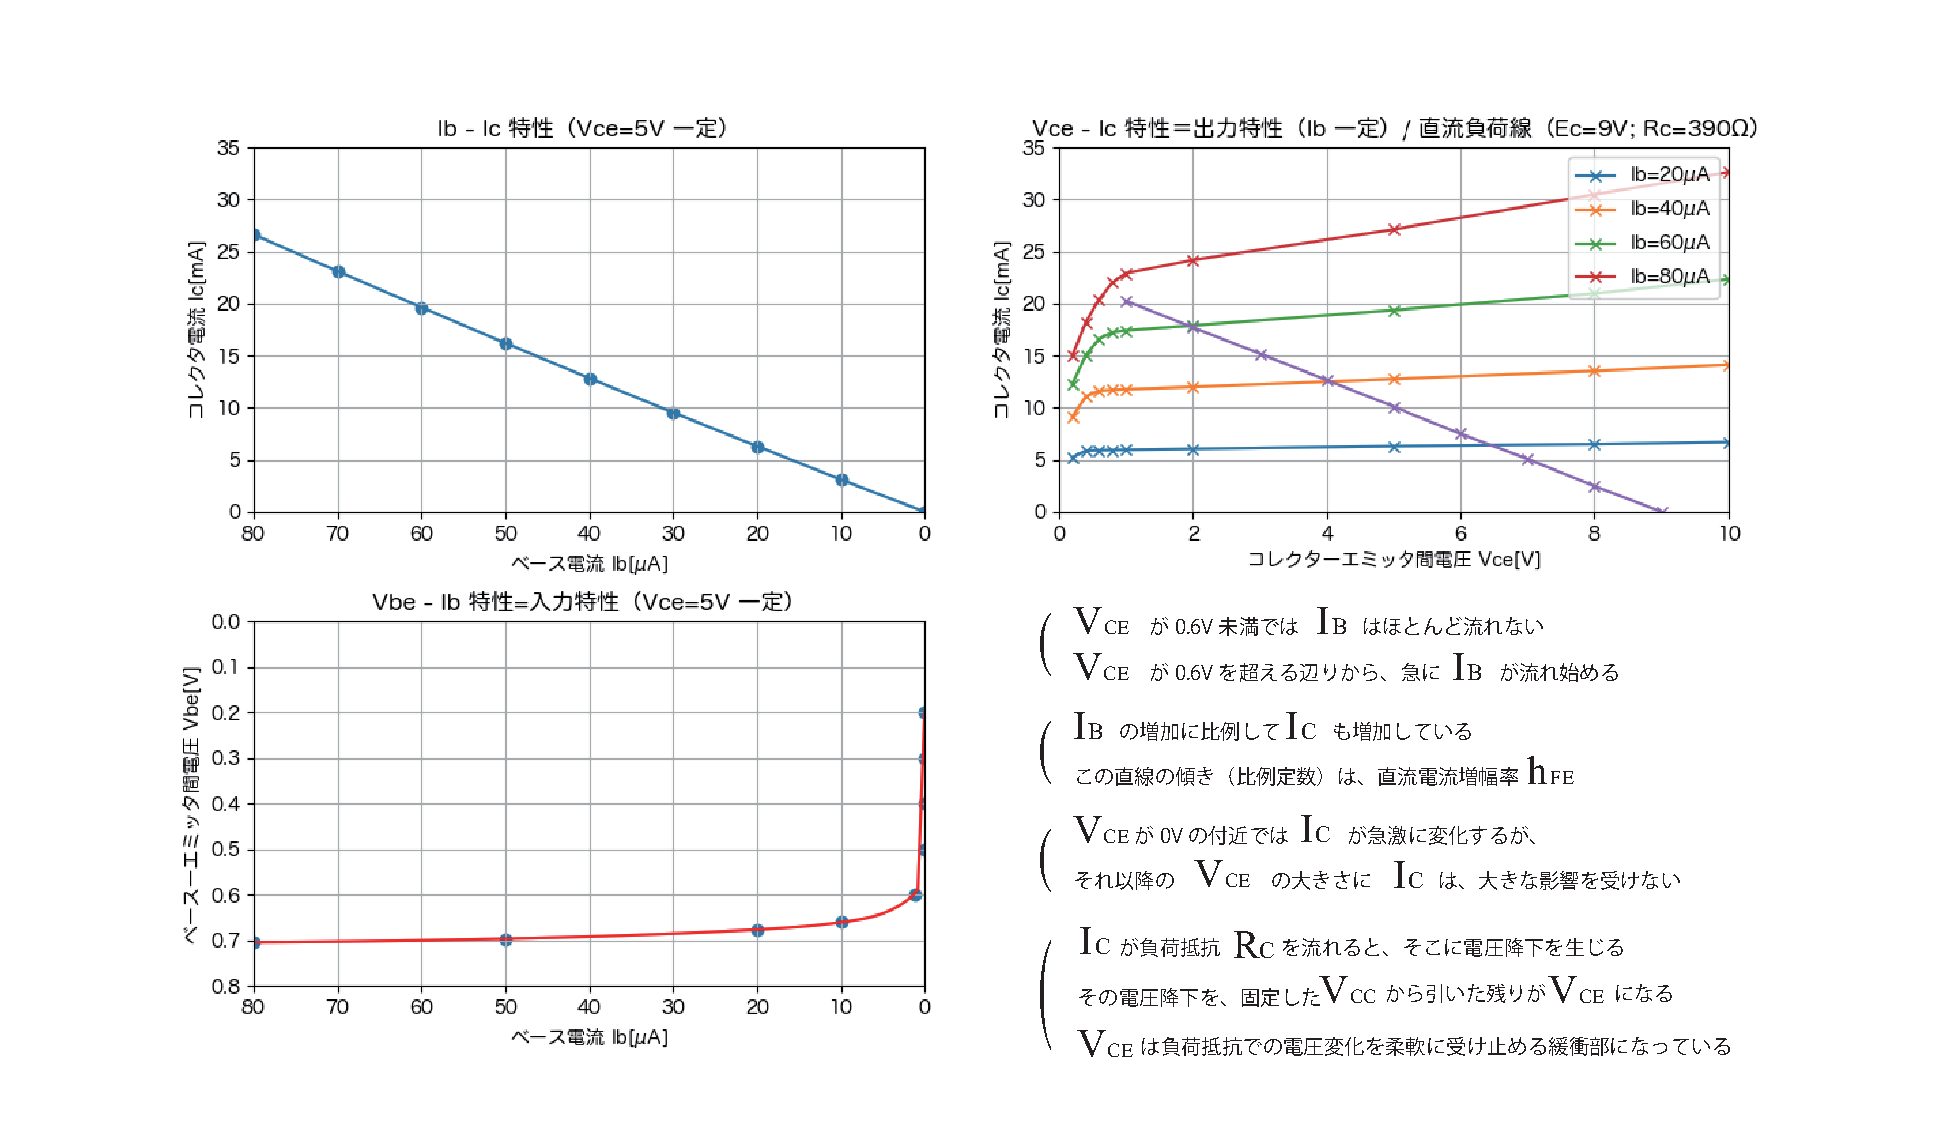
\includegraphics[keepaspectratio, scale=0.7, angle=90]
               {figs/eps/statictate.eps}
               \caption{作図例:トランジスタの静特性(2SC1815Y)}
               \label{fig:staticexample}
\end{figure}

\newpage

\chapter{低周波増幅回路}

\section{実習の目的}

エミッタ接地CR結合低周波一段増幅回路の諸特性を測定することを通して、
トランジスタを用いた増幅回路の特性及び動作原理を理解する。

\section{使用する機器}

\begin{itemize}
\item 回路計
\item トランジスタ(2SC1815-O、2SC1815Y, 2SC1815-GR、2SC1815-BL)\footnote{$I_C=1m$A となる様に$R_B$を調整すれば、どれでもOk!}
\item 低周波発振器
\item オシロスコープ
\item 直流安定化電源装置($V_{CC}$用)
\item 電子電圧計2台
\end{itemize}

\section{実習}

実習する項目
\begin{enumerate}
\item[(1)] 回路定数の設計について学習する\footnote{実教出版株式会社「電子回路」新訂版、第2章第5節「トランジスタによる小信号増幅回路の設計」}
\item[(2)] 実習装置について調べる
\item[(3)] 入出力特性を測定し、グラフを作成して特性を理解する
\item[(4)] 周波数特性を測定し、グラフを作成して特性を理解する
\end{enumerate}

\newpage

\subsection{回路定数の設計}

\begin{enumerate}
  \item まず$R_E$を決める\\
  \begin{itembox}[l]{設計条件}
  (1) コレクタ電流$I_C$には、$1$mA を流すことにする。\\
  (2) $V_{CC}$は、直流電源装置からの$DC12V$とする。\\
  (3) エミッタ抵抗$R_E$における電圧降下$V_E=V_{RE}$は、$V_{CC}$の$10\%$になる様にする。
  \end{itembox}
  \begin{enumerate}
  \item[(1)] 設計条件の(2)と(3)より、$V_{RE}=V_{CC}\times 0.1=$(   )V
  \item[(2)] $R_E$に流れる電流は、$I_E=I_B+I_C$になるが、実際には$I_B\ll I_C$であるから、$I_E\fallingdotseq I_C$と概算する。
  従って$R_E$の電流$I_E$も、$I_C$と同じ(   )$mA\;$だと考えられる。
  その時の$R_E$における電圧降下は$V_{RE}=$(   )Vだったから、$R_E=\displaystyle\frac{V_{RE}}{I_E}=$(   )$k\Omega$
  \end{enumerate}
  \vfill
  \item 次に、$R_C$を決める\\
  \begin{itembox}[l]{設計条件}
  (4)$V_{CE}\fallingdotseq V_{RC}$となる様に設計する。これにより最大値の大きな交流信号が得られる。
  \end{itembox}
  \begin{enumerate}
  \item[(1)] $V_{CC}=V_{RC}+V_{CE}+V_{RE}$で、$V_{CE}=V_{RC}$とおけば、
  $V_{RC}=\displaystyle\frac{V_{CC}-V_{RE}}{2}=$(   )V
  \item[(2)] 抵抗$R_C$の端子間電圧が上記の通りであり、これに流れる電流$I_C$は設計条件(1)で決められているので、
  $R_C=\displaystyle\frac{V_{RC}}{I_C}=$(   )$k\Omega$だが、E系列\footnote{抵抗値と静電容量値には、いくつかの標準数列が規定され、推奨されている。標準数列のE24系列の数値は次の通り。\\
  $1.0\;\;1.1\;\;1.2\;\;1.3\;\;1.5\;\;1.6\;\;1.8\;\;2.0\;\;2.2\;\;2.4\;\;2.7\;\;3.0\;\;3.3\;\;3.6\;\;3.9\;\;4.3\;\;4.7\;\;5.1\;\;5.6\;\;6.2\;\;6.8\;\;7.5\;\;8.2\;\;9.1$}
  の数値から$R_C=5.6k\Omega$を選ぶ
  \end{enumerate}
  \vfill
  \item ブリーダ抵抗$R_A$を決める\\
  \begin{itembox}[l]{設計条件}
  (5) 使用するトランジスタの直流電流増幅率を$h_{FE}\fallingdotseq 180$とする。\\
  (6) このトランジスタのベース−エミッタ間の電圧は$V_{BE}\fallingdotseq 0.6V$とする。\\
  (7) $R_A$にはベース電流$I_B$の20倍の電流(ブリーダ電流$I_A$)を流すことにする。
  \end{itembox}
  \begin{enumerate}
  \item[(1)] コレクタ電流$I_C$に$1mA$を流す時のベース電流$I_B$は、
  $I_B=\displaystyle\frac{I_C}{h_{FE}}=$(    )$\mu A$
  \item[(2)] 設計条件(7)よりブリーダ電流は、$I_A=20\times I_B=$(    )$\mu A$
  %\item[(3)] $R_B$に流れる電流$I_B$は、$R_A$に流れる電流$I_A$とベースに流れる電流$I_B$の和になる
  \item[(3)] ベース電位は$V_B=V_{BE}+V_{RE}$であるから、$V_B=(   )+(   )$=(   )$V$
  \item[(4)] この値$V_B$は、$R_A$にブリーダ電流$I_A$が流れることによる電圧降下$V_{RA}$に等しいから、\\
  $R_A=\displaystyle\frac{V_{RA}}{I_A}=\frac{V_B}{I_A}=$(   )$k\Omega$
  \end{enumerate}
  \vfill
  \item 最後に、$R_B$を決める
  \begin{enumerate}
  \item[(1)] ブリーダ抵抗$R_A$と$R_B$は$V_{CC}$を分圧しているので、
  $V_{RB}=V_{CC}-V_{RA}=$(    )$V$
  \item[(2)] $R_B$にはブリーダ電流$I_A$とベース電流$I_B$の両方$I_A+I_B=$(    )$\mu A$が流れるので、
  $V_{RB}=R_B\cdot(I_A+I_B)$より、$R_B=\displaystyle\frac{V_{RB}}{I_A+I_B}\fallingdotseq$(    )$k\Omega$
  \item[(3)] E系列の数値から、$R_B=91k\Omega$を選ぶことにする
  %が、コレクタ電流を$I_C=1mA$に調整できる様にするため、\\
  %$R_B$には、E系列の$82k\Omega$に半固定抵抗の$50k\Omega$を直列に接続することも考えられる
  \end{enumerate}
\end{enumerate}

%\newpage

\begin{figure}[H]
  \centering
   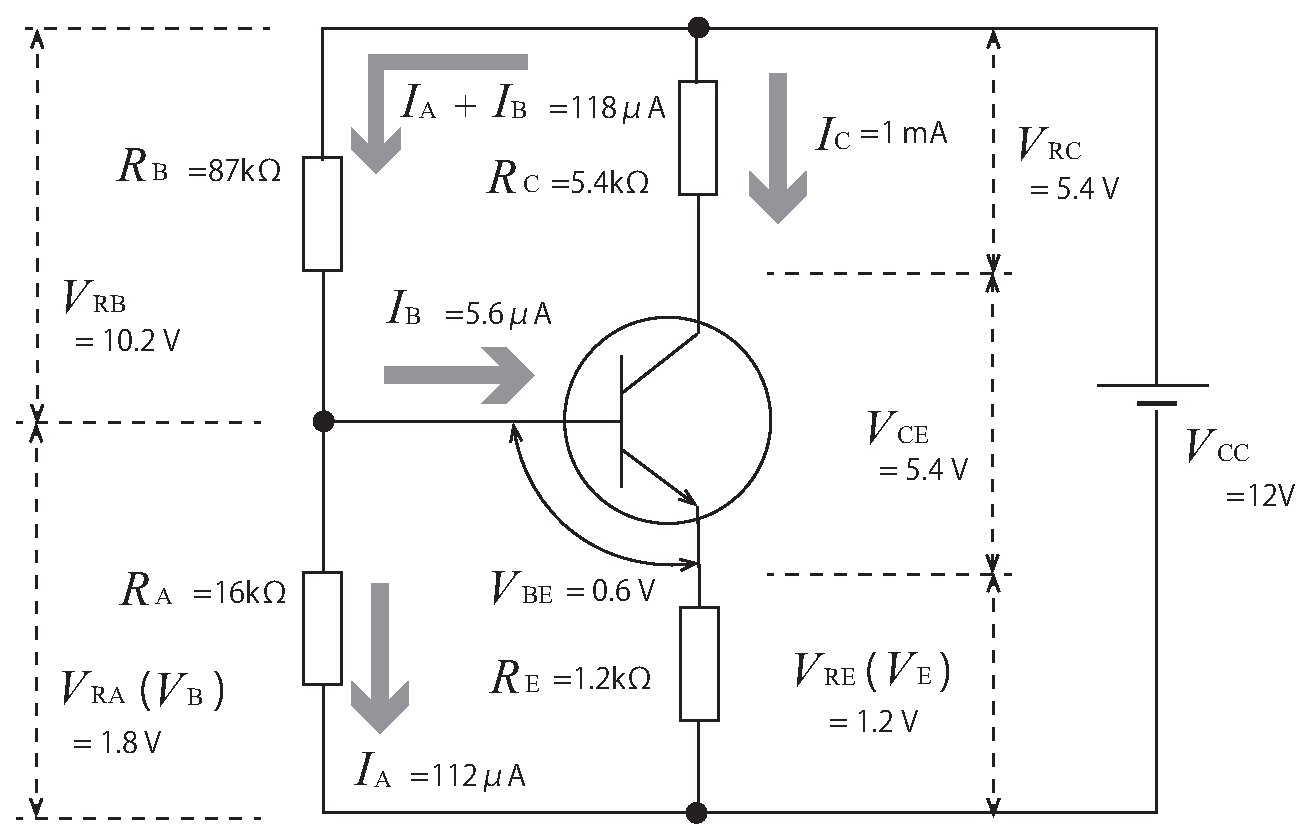
\includegraphics[keepaspectratio, scale=0.45, angle=0]
               {figs/eps/p96fig3a.eps}
               \caption{回路定数を算出した時の値}
               \label{fig:11_2}
\end{figure}

\subsection{実習装置について調べる}

回路計を使って以下の手順で測定し、図\ref{fig:11_1}と表\ref{tbl1}に測定した値を記録する

\begin{enumerate}
\item[(1)] 表\ref{tbl1}の項番の1〜6を測定し記録する。(実習装置からTrは取り外し、電源装置も繋がない)
\item[(2)] Trの名前を読み取って記録し、そのトランジスタについて調査したことをレポートに報告する
\item[(3)] 抵抗器のカラーコードなどを読み取り、その抵抗器の公称値を調べ、実測値と比較する
\item[(4)] ここでTrを実習装置にセットし、また直流電源装置を12Vに設定して実習装置に給電する
\item[(5)] Trの3つの端子を使って、表\ref{tbl1}の項番7〜12の電圧を回路計で直接測定する
\item[(6)] 設計時の条件や目標値と、実際に測定した値とを比較する
\end{enumerate}

実習装置で使っているトランジスタの外観、及び名盤の表記をスケッチし、
トランジスタの図記号、端子の名称、各端子を流れる電流の呼称と表記、
端子間電圧の呼称と表記について調べて記録する\\

\begin{comment}
	\begingroup
	\renewcommand{\arraystretch}{1.4}
	\begin{table}[H]
		\begin{center}
			\caption{トランジスタについて調べる(外観、端子、名称)}%\label{tbl:t1}\vspace{2mm}
			\begin{tabular}{|wl{6cm}|wl{6cm}|} \hline
				外観のスケッチ & トランジスタの名称\\
				& \\
				& 左の端子の名称\\
				& \\
				& 真ん中の端子の名称\\
				& \\
				& 右の端子の名称\\
				& \\ \hline
			\end{tabular}
		\end{center}
	\end{table}
	\endgroup
\end{comment}

\begin{figure}[H]
	\centering
	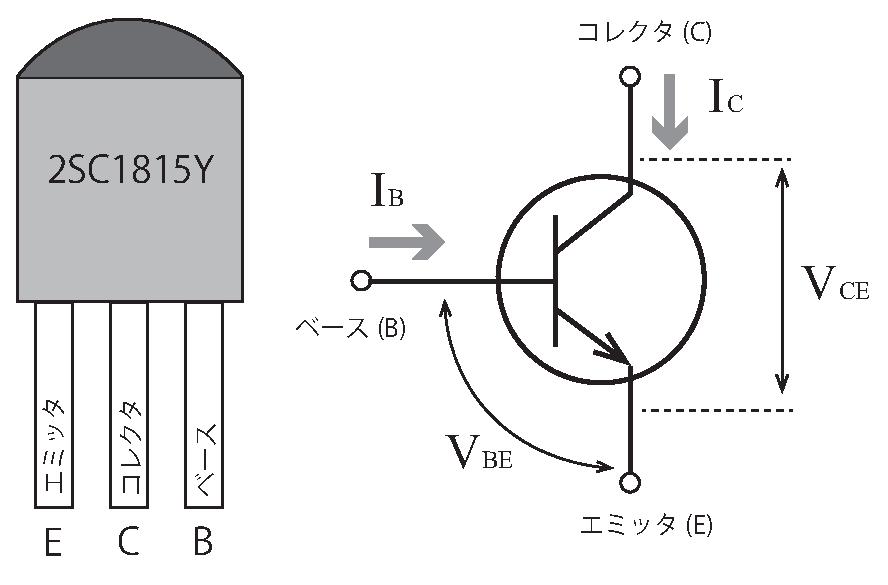
\includegraphics[keepaspectratio, scale=0.6, angle=0]
	{figs/eps/illust.eps}
	%\caption{}
	\label{fig:illust}
\end{figure}

\newpage

\begingroup
\renewcommand{\arraystretch}{1.2}
\begin{table}[H]
  \begin{center}
  \caption{回路計による実測値}\label{tbl1}
  \begin{tabular}{|c|l|wr{2.2cm}|l|} \hline
    \multicolumn{1}{|c|}{\textbf{項番}} & \multicolumn{1}{c|}{\textbf{項目}} & \multicolumn{1}{c|}{\textbf{実測値}} & \multicolumn{1}{c|}{\textbf{備考(公称値など)}} \\ \hline
    1 & $R_E$ & $\;k\Omega$ & カラーコード(       )、($       )$$\Omega$ \\
    2 & $R_C$ & $\;k\Omega$ & カラーコード(       )、($       )$$\Omega$ \\
    3 & $R_A$ & $\;k\Omega$ & カラーコード(       )、($       )$$\Omega$ \\
    4 & $R_B$ & $\;k\Omega$ & 半固定抵抗器 表記(   )、$20\times 10^2\Omega$ \\
    5 & $V_{CC}$ & $\;V$ & 直流安定化電源装置(DC12V) \\
    6 & $h_{FE}$ & $\;$ & Trの名称は(          )\\ \hline
    7 & $V_{RC}$ & $\;V$ & 設計時の目標は$V_{RC}\fallingdotseq V_{CE}=(V_{CC}-V_{RE})/2$だけど?\\
    8 & $V_{CE}$ & $\;V$ & $V_{RC}\fallingdotseq V_{CE}$で最大値の大きな交流信号出力が得られる\\
    9 & $V_{BE}$ & $\;V$ & シリコンTrの値になっているかな?\\
    10 & $V_{RE}$ & $\;V$ & 設計時の条件、$V_{CC}$の$10\%=$(   )Vになってる?\\
    11 & $V_{RA}$ & $\;V$ & $V_{BE}+V_{RE}=$(     )Vと比べてどうかな? \\
    12 & $V_{RE}+V_{CE}$ & $\;V$ & $V_{CC}-V_{RC}=$(     )Vと比べてどうかな? \\ \hline
  \end{tabular}
  \end{center}
\end{table}
\endgroup

\vfill

\begin{figure}[H]
  \centering
   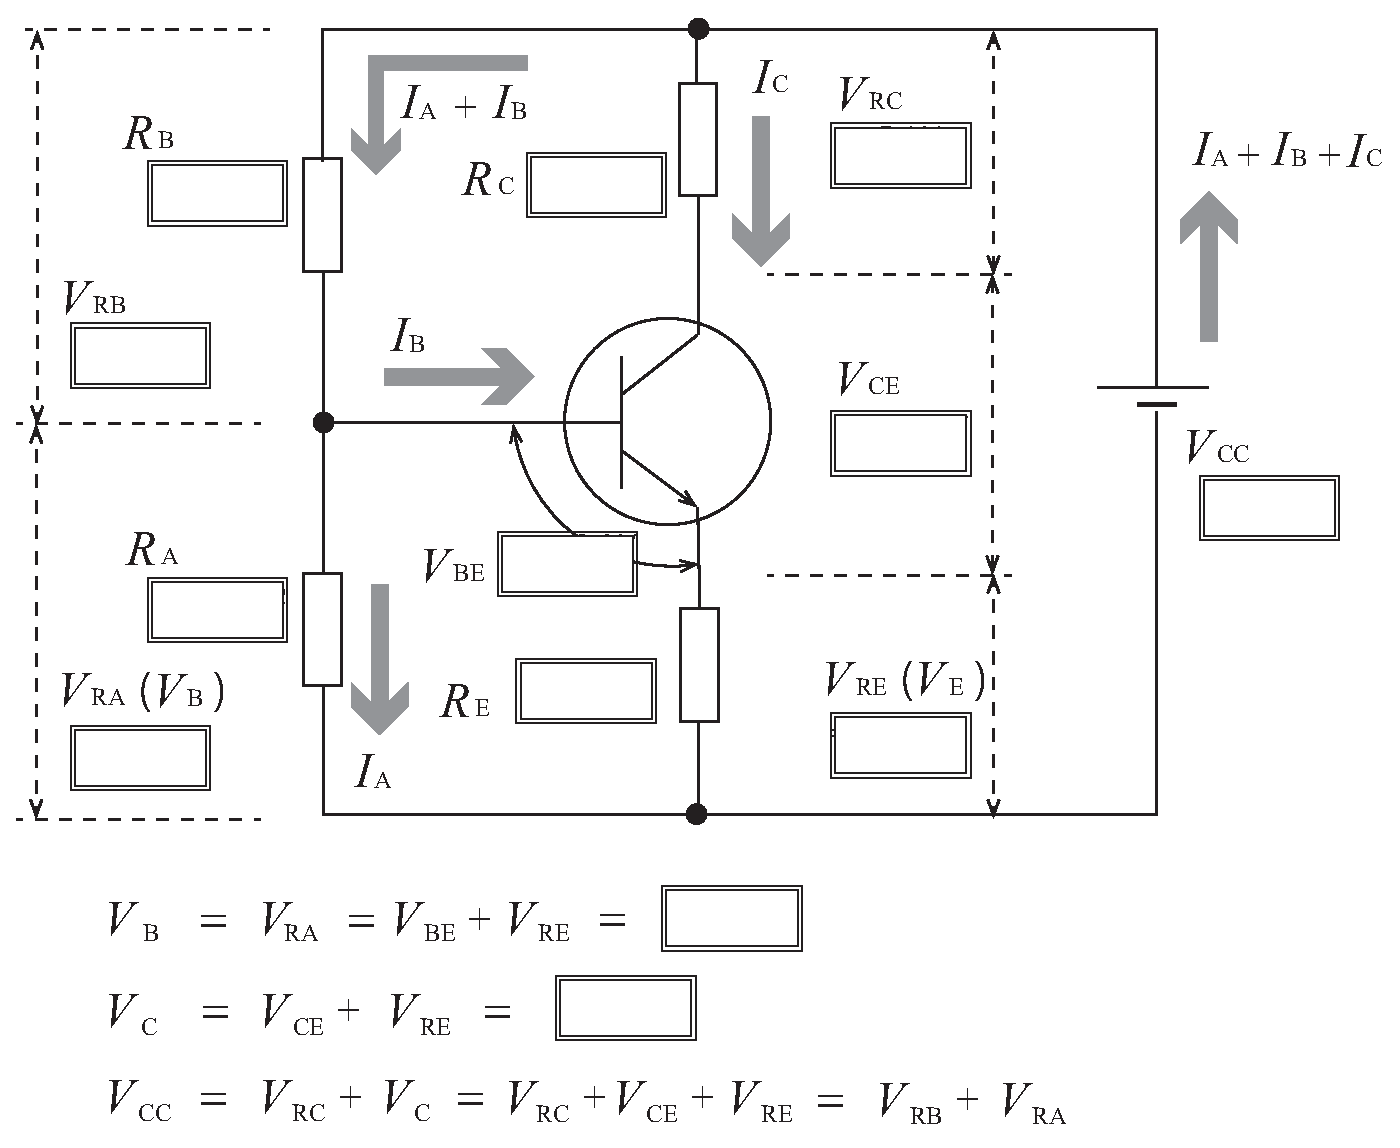
\includegraphics[keepaspectratio, scale=0.58, angle=0]
               {figs/eps/p96fig3b.eps}
               \caption{実際の回路で測定した時の値}
               \label{fig:11_1}
\end{figure}

\newpage

\subsection{入出力特性を測定する}

入出力特性(オシロスコープで入力波形および出力波形を観察、記録する)

\begin{enumerate}
\item[(1)] 電源電圧を$E_C(V_{CC})=12$Vとし、発振器の周波数を$1k$Hz 一定の正弦波とする
\item[(2)] 入力電圧$V_i$を増加させ、その時の出力電圧$V_o$の値を記録する
\item[(3)] 電圧増幅度($A_V=V_o/V_i$)を計算する
\item[(4)] 入出力特性(入力電圧ー出力電圧)をグラフに表す 
\item[(5)] グラフの直線部分を直線のまま延伸し、実測値と離れる時の入力電圧を読み取る
\item[(6)] その時の入力電圧の前後で、出力波形に歪みを生じ始めていることを確認する
\end{enumerate}

%\begin{spacing}{0.67}
%  \begin{multicols}{2}
  \begin{figure}[H]
    \centering
     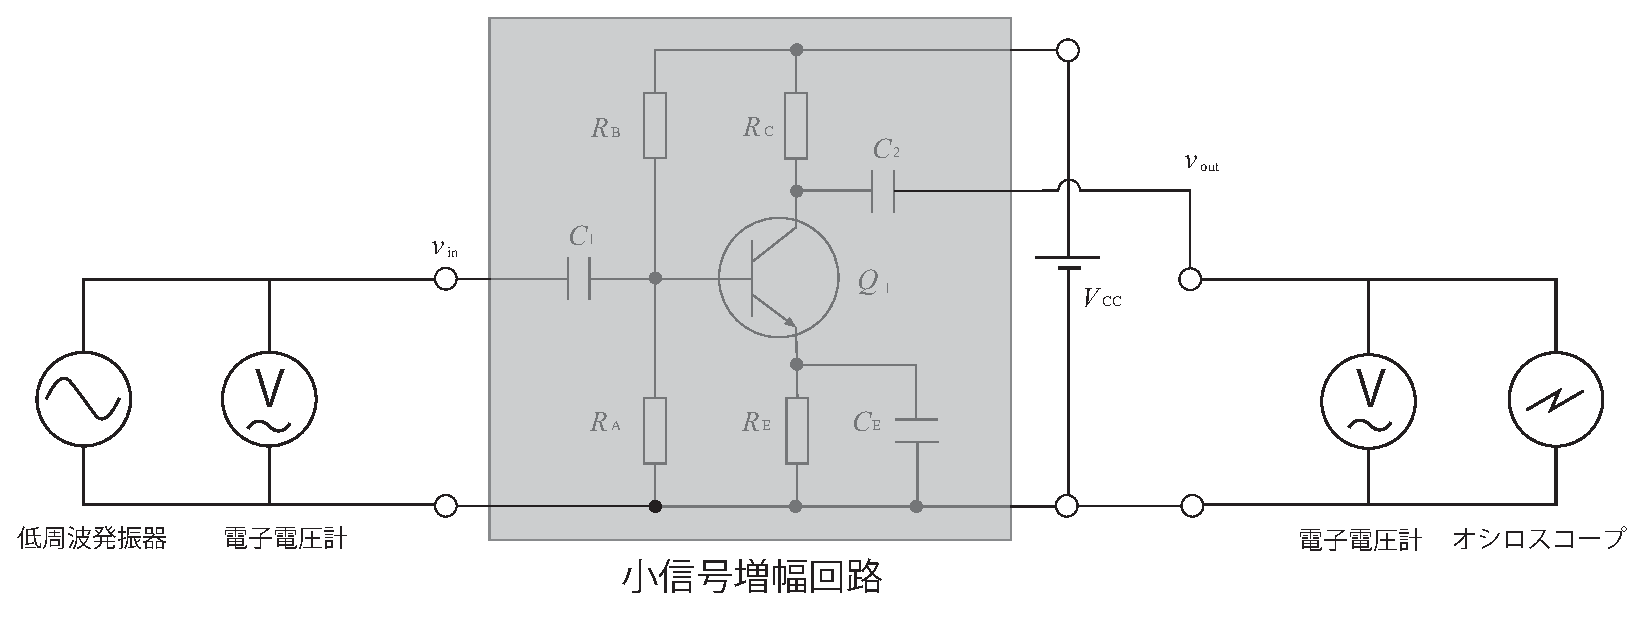
\includegraphics[keepaspectratio, scale=0.48, angle=0]
               {figs/eps/exp0.eps}
               \caption{実習装置}
               \label{fig:exp0}
 \end{figure}
 
%入出力特性のグラフ作図例

 \begin{figure}[H]
    \centering
     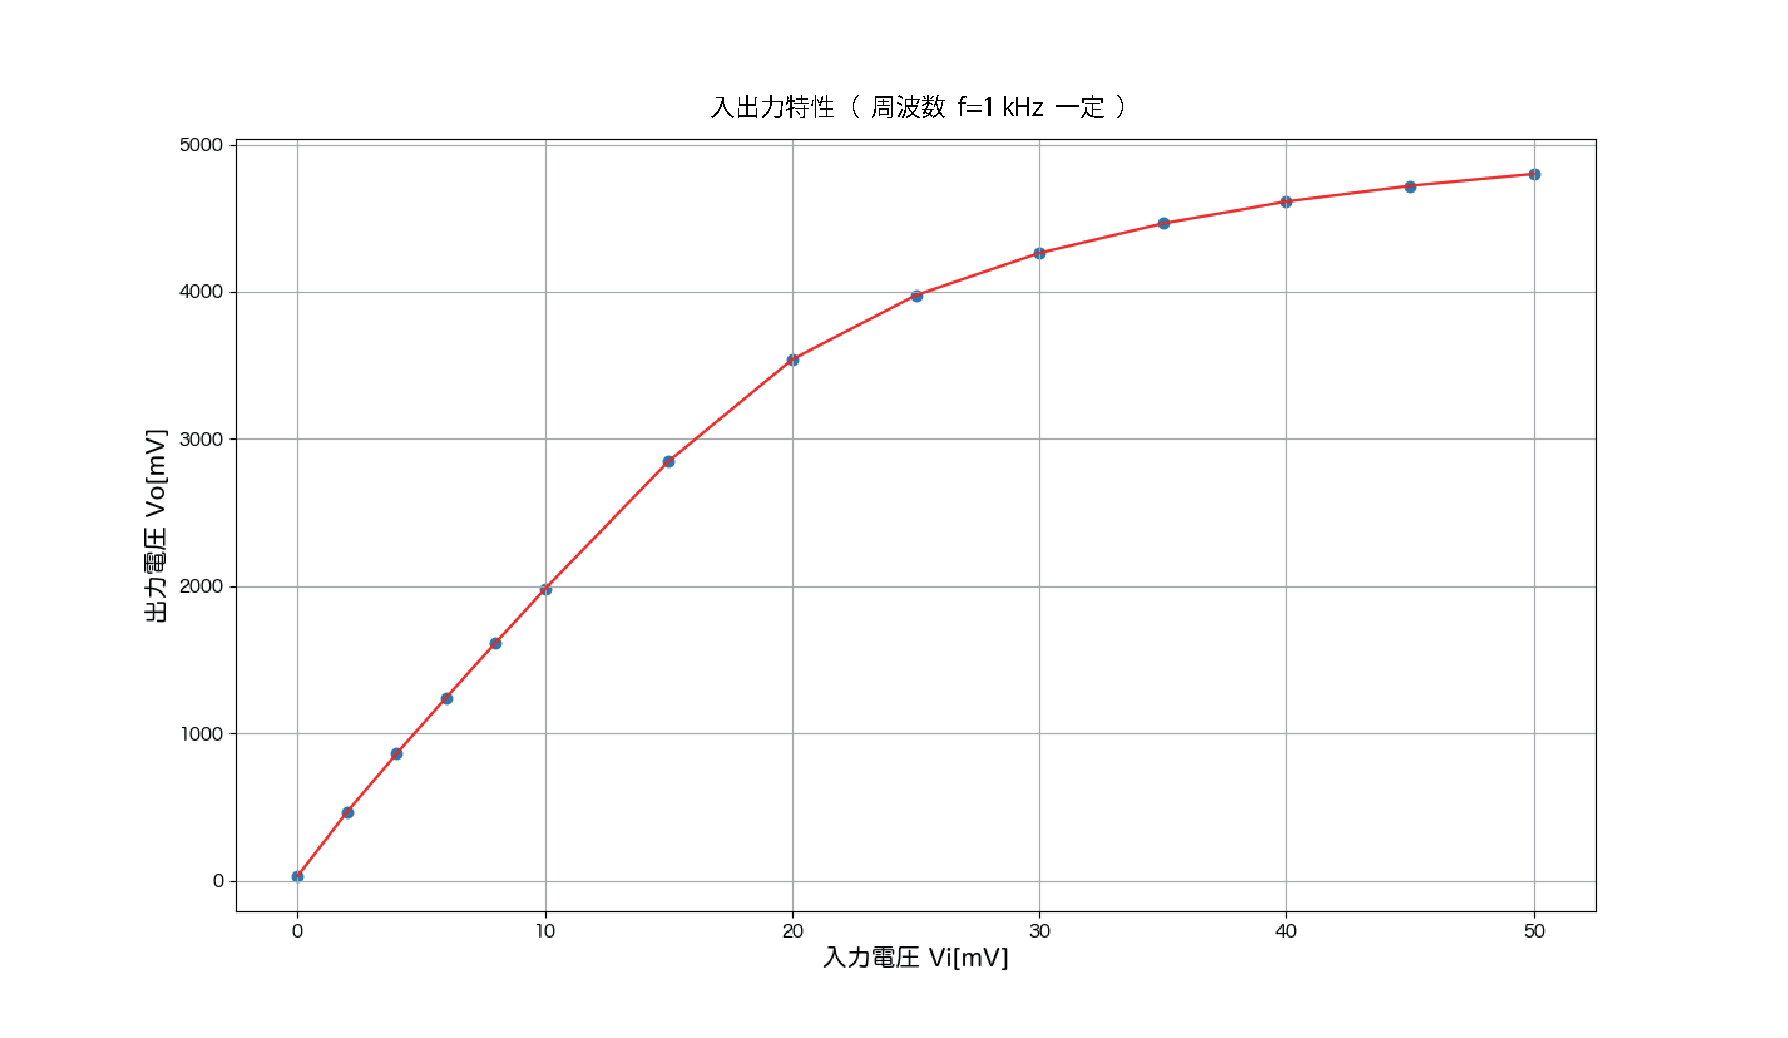
\includegraphics[keepaspectratio, scale=0.55, angle=0]
                 {figs/eps/iocharM1YExample.eps}
                 \caption{入出力特性のグラフ作成例}
                 \label{fig:iocharM1Yd}
 \end{figure}
%  \end{multicols}
%\end{spacing}

\newpage

\begin{figure}[H]
  \centering
   \includegraphics[keepaspectratio, scale=0.76, angle=90]
               {figs/eps/iokiroku.eps}
               \caption{入出力特性の記録用紙}
               \label{fig:22_1}
\end{figure}

\newpage

【入出力特性:オシロスコープ画面の情報をスケッチせよ】

\begin{multicols}{2}
  \begin{figure}[H]
     \centering
      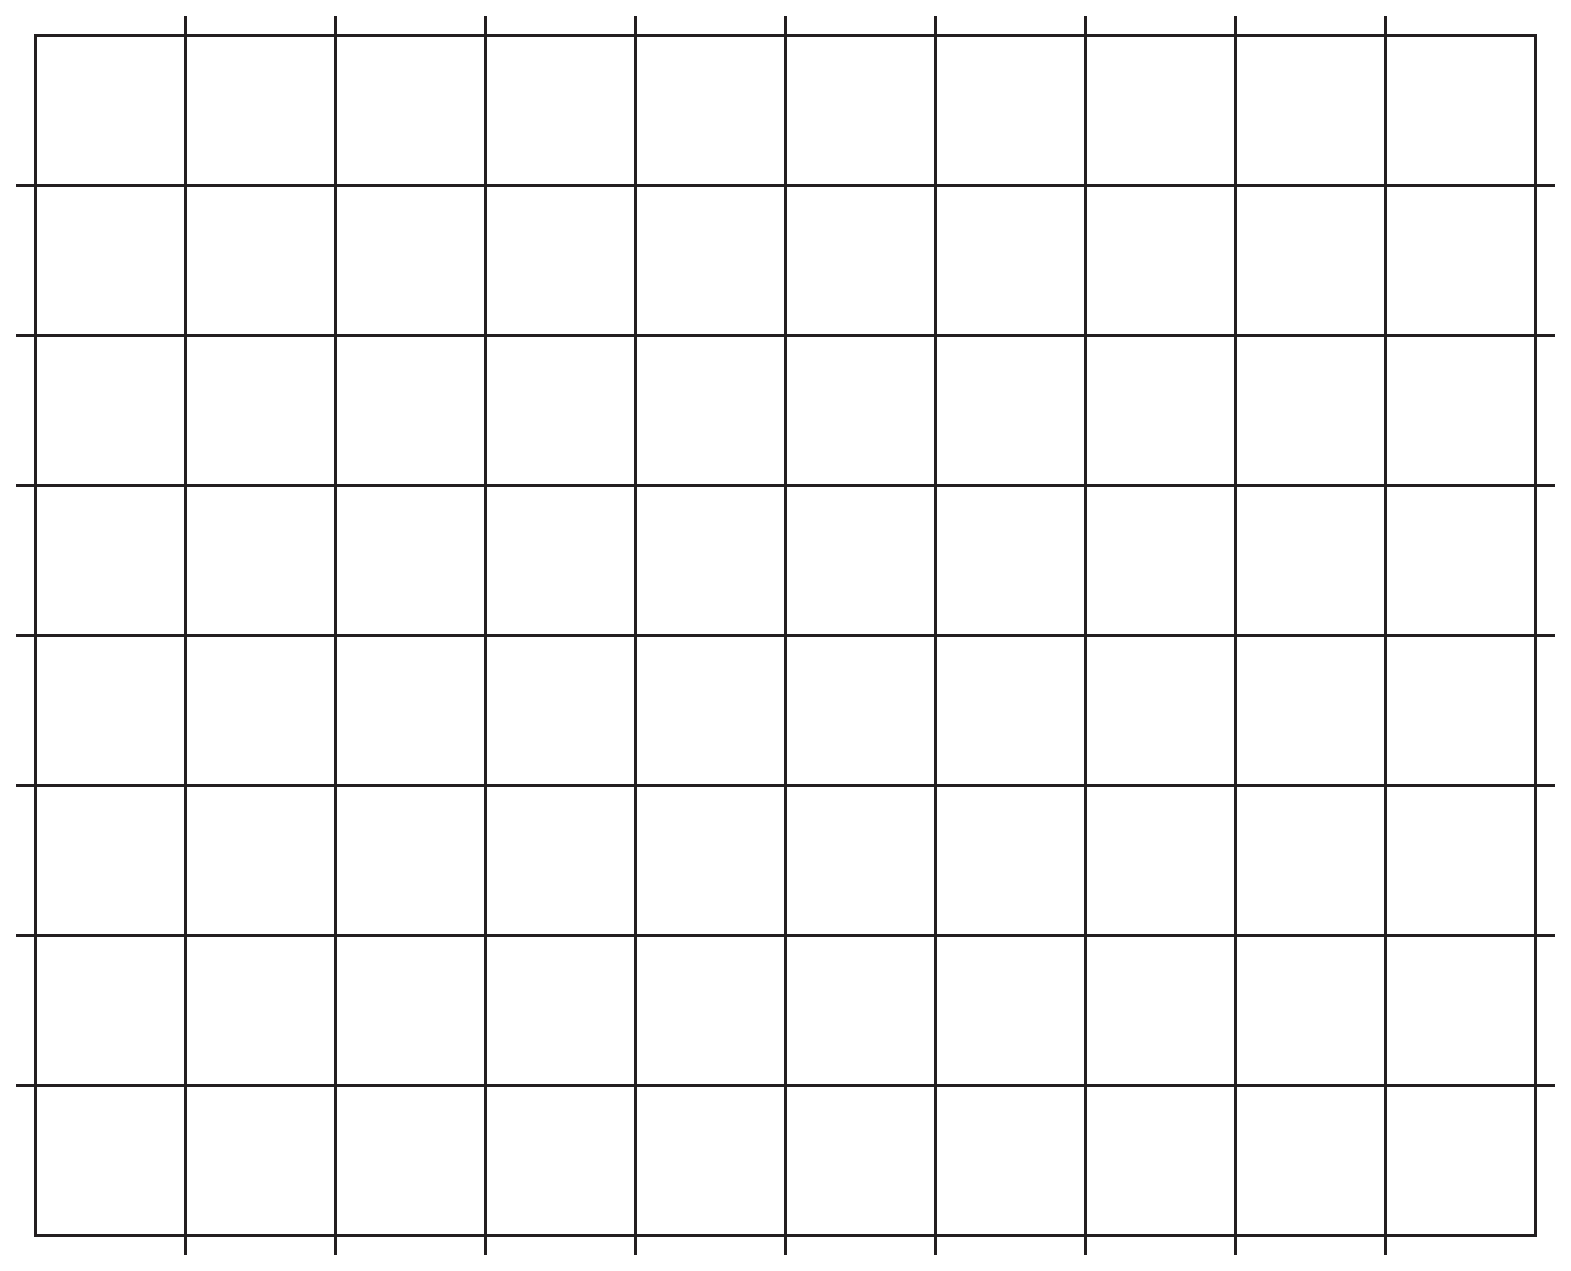
\includegraphics[keepaspectratio, scale=0.28, angle=0]
                  {figs/eps/grid.eps}
                  %\caption{オシロスコープの画面スケッチ}
                  \label{fig:grid6mV}
  \end{figure}

  \begin{spacing}{1.5}
  \begin{tabular}{|c||r|r|r|}
    \multicolumn{4}{c}{入力(実効値)$V_i=6\;$mVの時の出力} \\ \hline
    項目 & DIVs & Value/DIV & Value \\ \hline \hline
    振幅pp &      & 2.0[V]&      \\ \hline
    波長 &      & 200.0[$\mu$s]&      \\ \hline
  \end{tabular}
\end{spacing}
\end{multicols}

\vfill

\begin{multicols}{2}
  \begin{figure}[H]
     \centering
      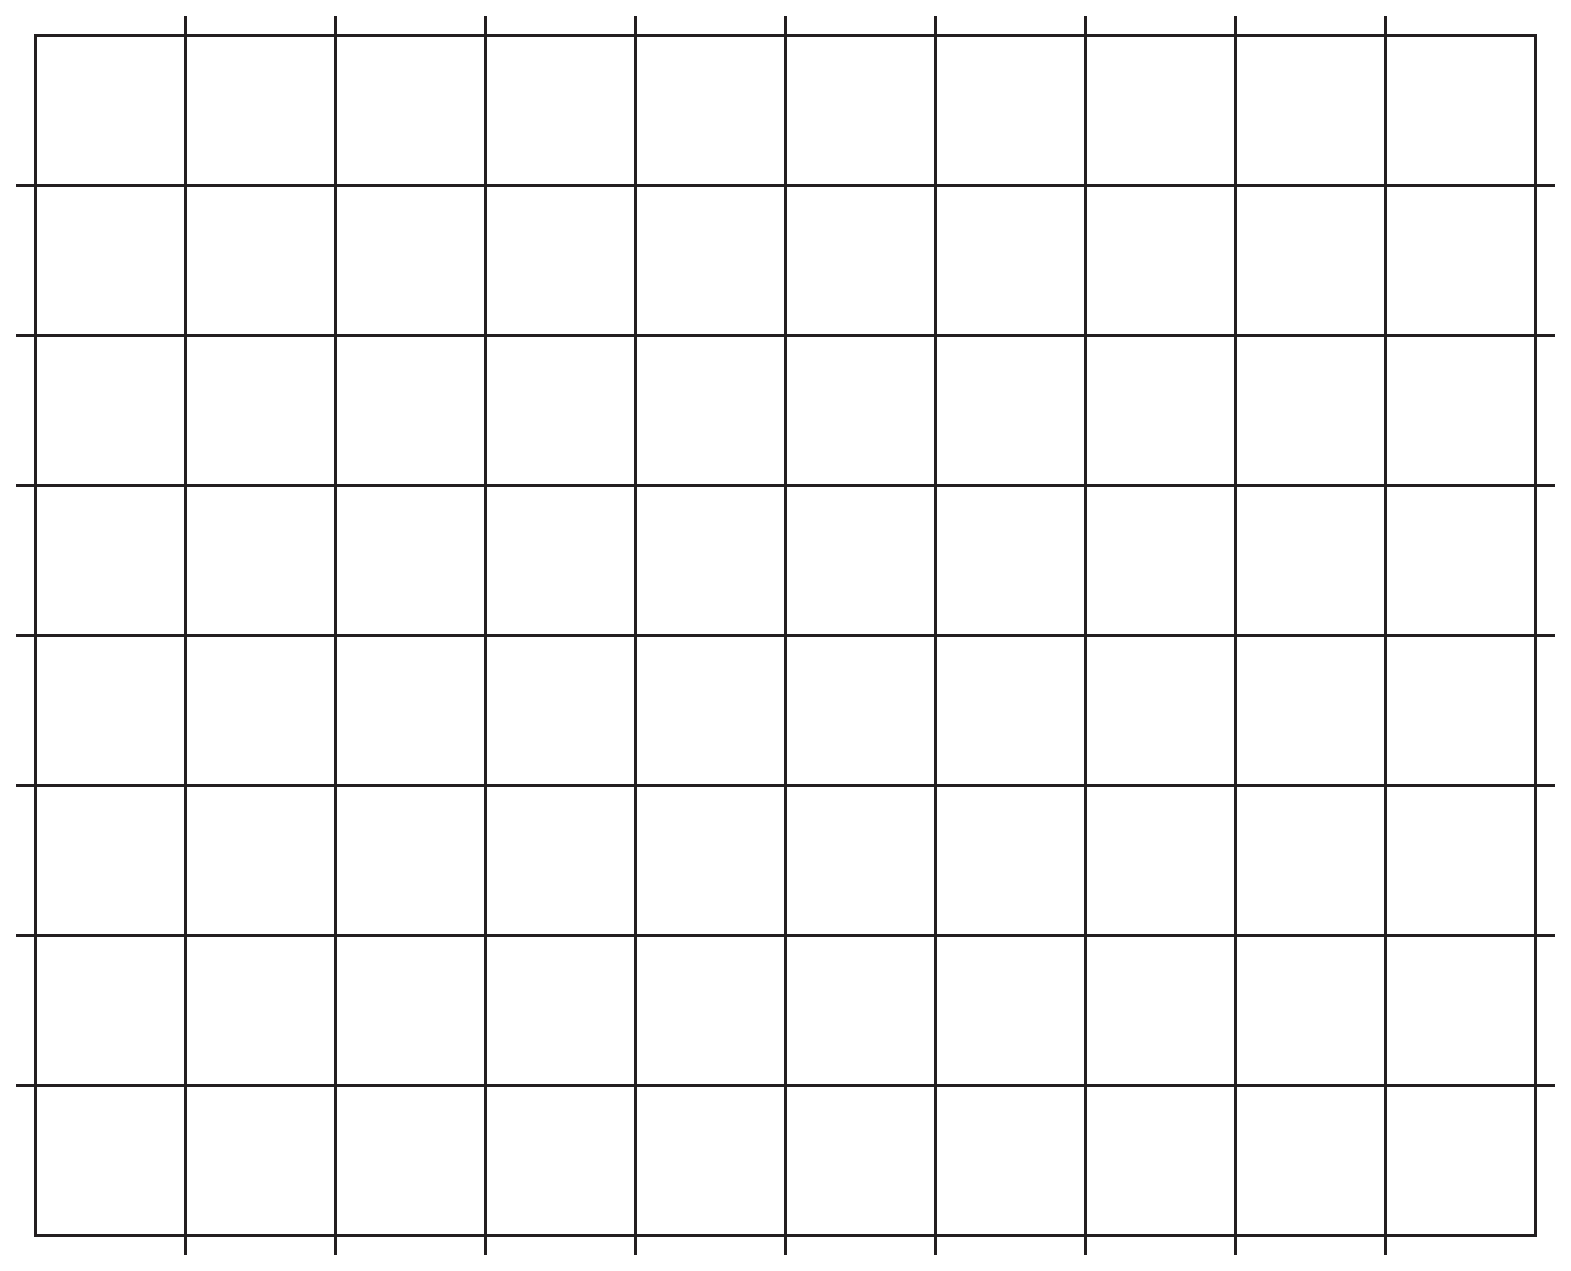
\includegraphics[keepaspectratio, scale=0.28, angle=0]
                  {figs/eps/grid.eps}
                  %\caption{オシロスコープの画面スケッチ}
                  \label{fig:grid10mV}
  \end{figure}

  \begin{spacing}{1.5}
  \begin{tabular}{|c||r|r|r|}
    \multicolumn{4}{c}{入力(実効値)$V_i=10\;$mVの時の出力} \\ \hline
    項目 & DIVs & Value/DIV & Value \\ \hline \hline
    振幅pp &      & 2.0[V]&      \\ \hline
    波長 &      & 200.0[$\mu$s]&      \\ \hline
  \end{tabular}
\end{spacing}
\end{multicols}

\vfill

\begin{multicols}{2}
  \begin{figure}[H]
     \centering
      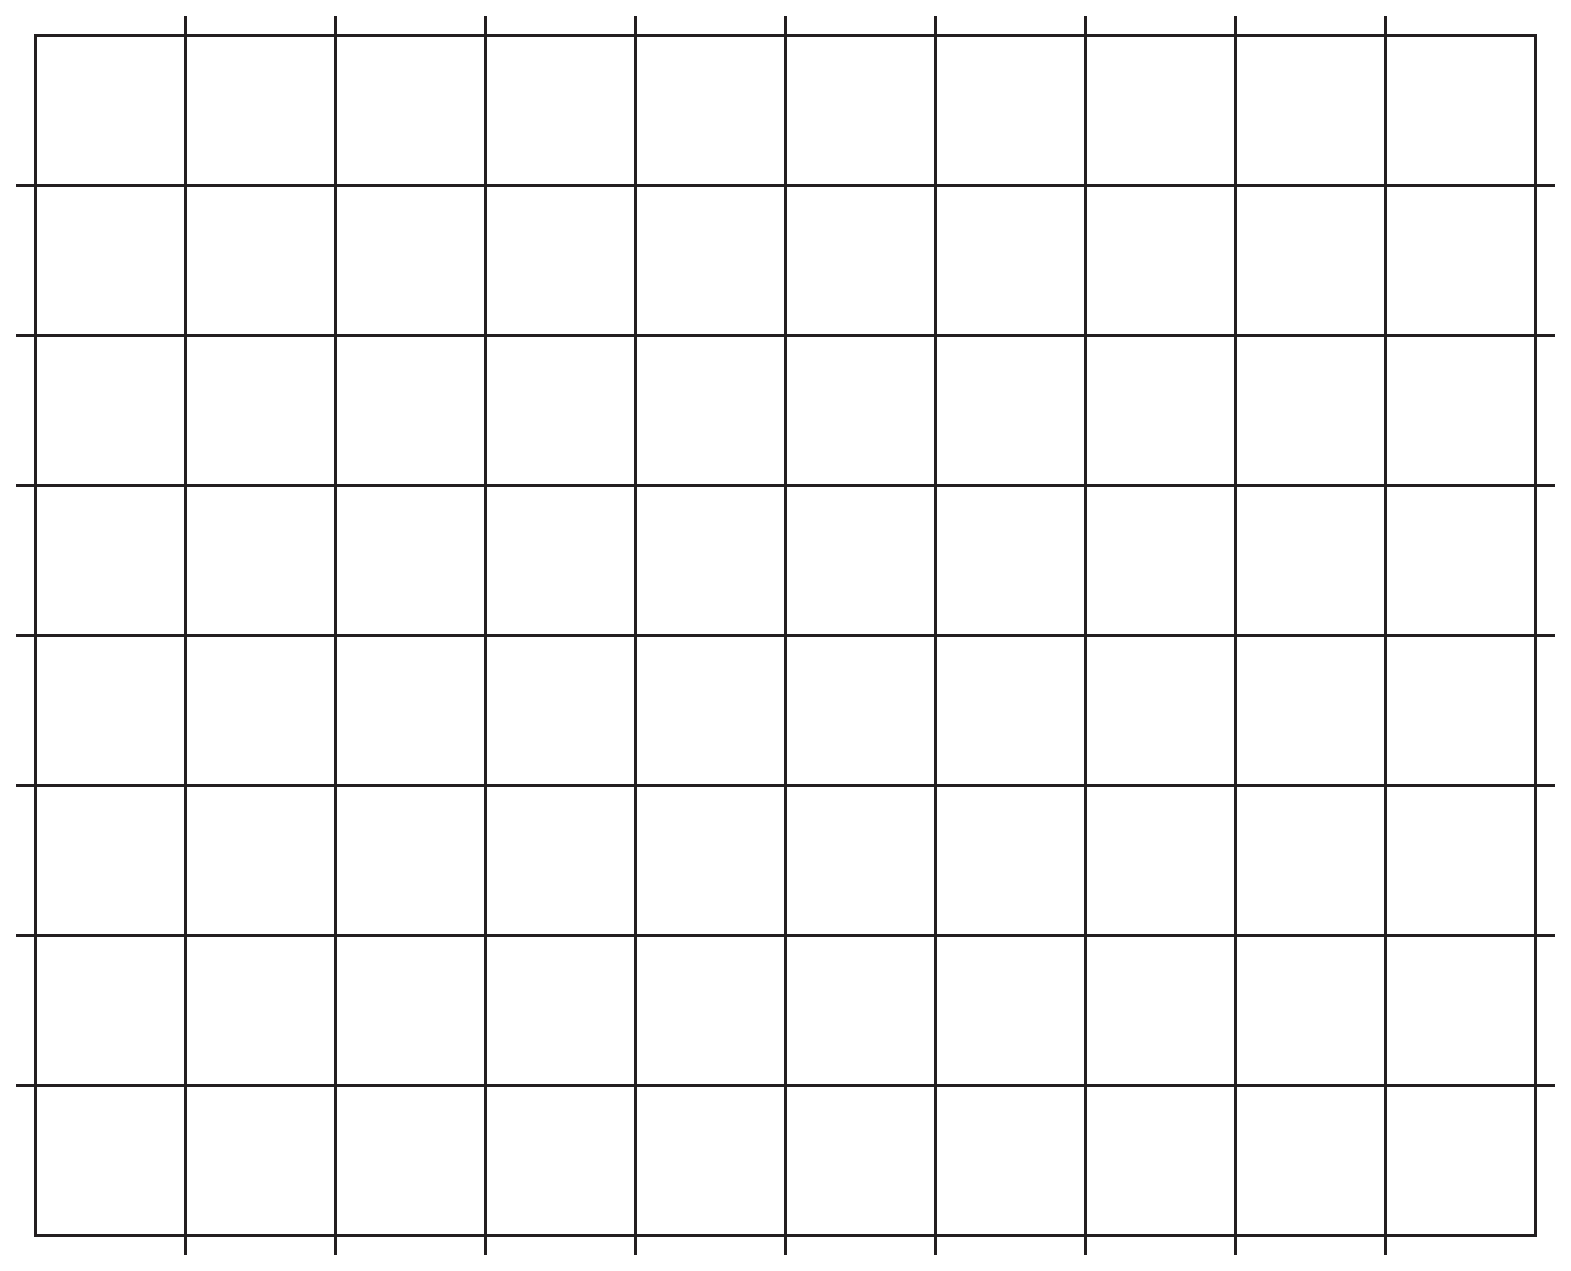
\includegraphics[keepaspectratio, scale=0.28, angle=0]
                  {figs/eps/grid.eps}
                  %\caption{オシロスコープの画面スケッチ}
                  \label{fig:grid20mV}
  \end{figure}

  \begin{spacing}{1.5}
  \begin{tabular}{|c||r|r|r|}
    \multicolumn{4}{c}{入力(実効値)$V_i=20\;$mVの時の出力} \\ \hline
    項目 & DIVs & Value/DIV & Value \\ \hline \hline
    振幅pp &      & 5.0[V]&      \\ \hline
    波長 &      & 200.0[$\mu$s]&      \\ \hline
  \end{tabular}
\end{spacing}
\end{multicols}

\vfill
\newpage

\begin{multicols}{2}
  \begin{figure}[H]
     \centering
      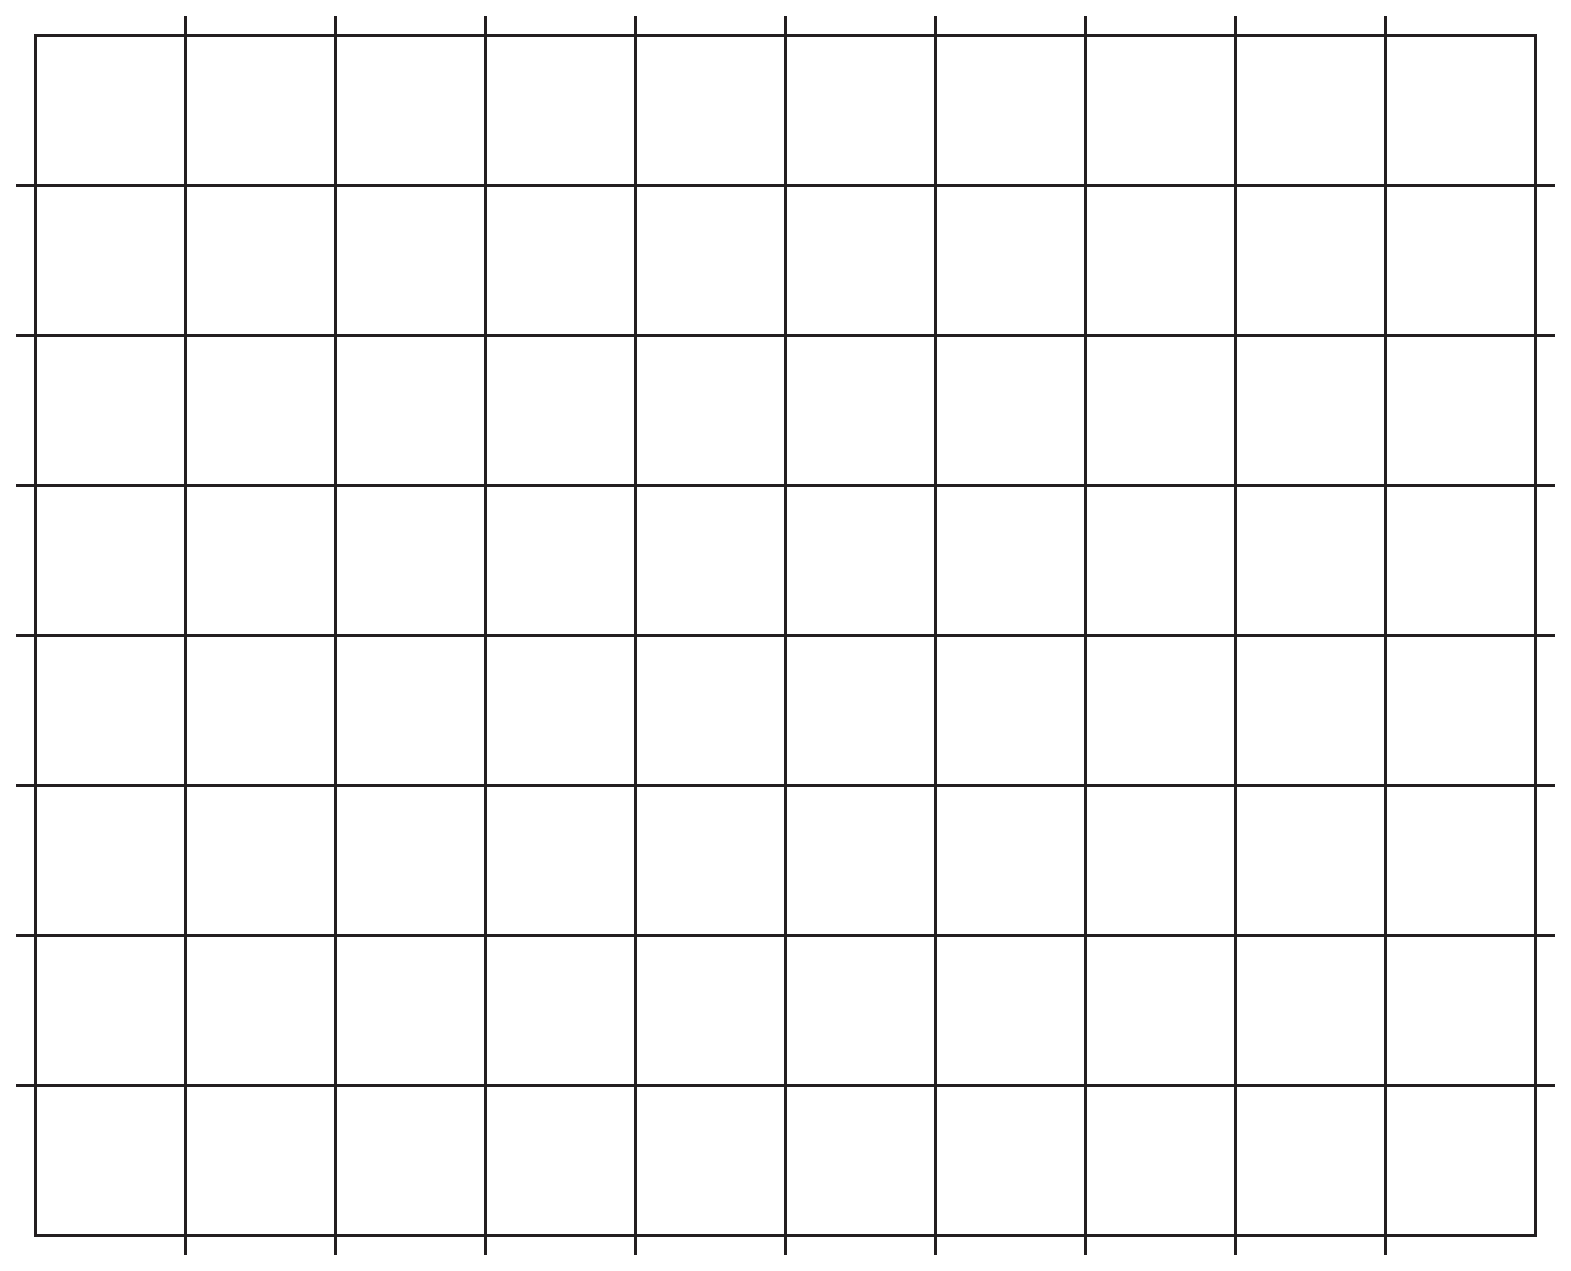
\includegraphics[keepaspectratio, scale=0.28, angle=0]
                  {figs/eps/grid.eps}
                  %\caption{オシロスコープの画面スケッチ}
                  \label{fig:grid30mV}
  \end{figure}

  \begin{spacing}{1.5}
  \begin{tabular}{|c||r|r|r|}
    \multicolumn{4}{c}{入力(実効値)$V_i=30\;$mVの時の出力} \\ \hline
    項目 & DIVs & Value/DIV & Value \\ \hline \hline
    振幅pp &      & 5.0[V]&      \\ \hline
    波長 &      & 200.0[$\mu$s]&      \\ \hline
  \end{tabular}
\end{spacing}
\end{multicols}

\vfill

\begin{multicols}{2}
  \begin{figure}[H]
     \centering
      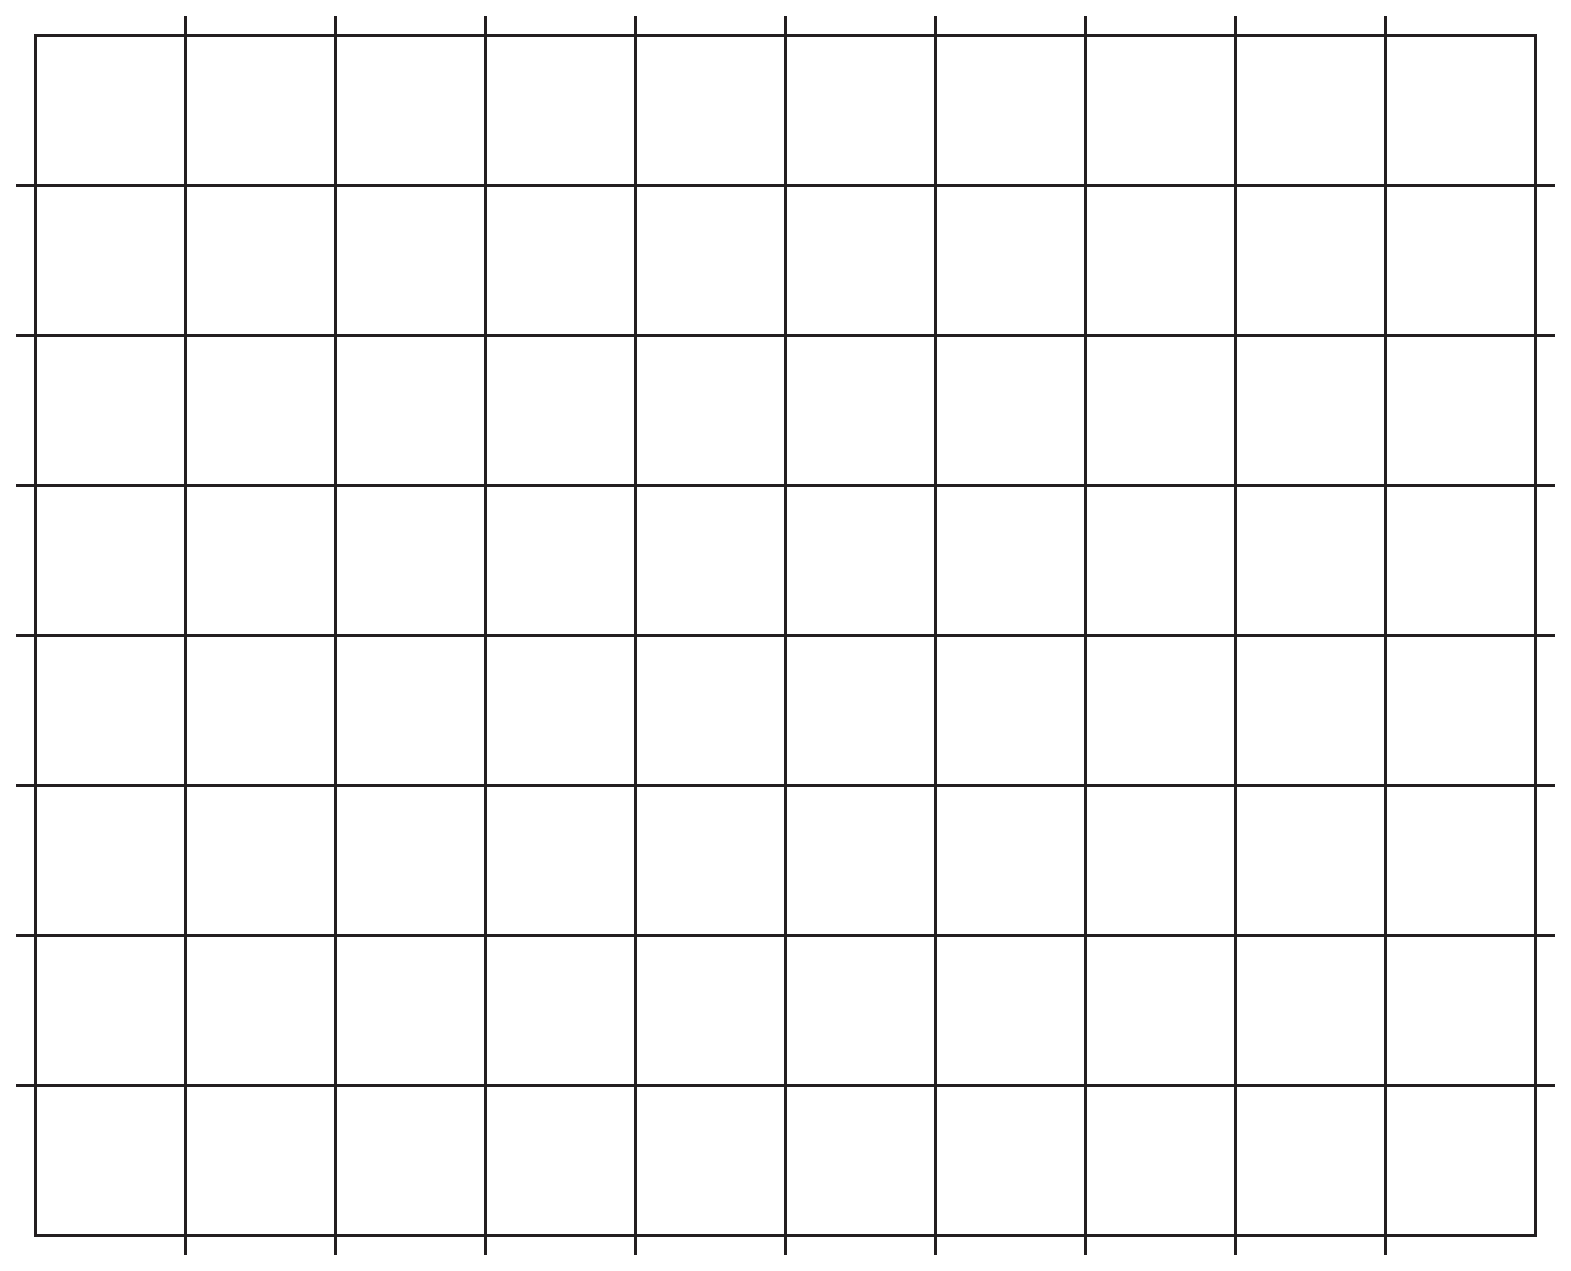
\includegraphics[keepaspectratio, scale=0.28, angle=0]
                  {figs/eps/grid.eps}
                  %\caption{オシロスコープの画面スケッチ}
                  \label{fig:grid40mV}
  \end{figure}

  \begin{spacing}{1.5}
  \begin{tabular}{|c||r|r|r|}
    \multicolumn{4}{c}{入力(実効値)$V_i=40\;$mVの時の出力} \\ \hline
    項目 & DIVs & Value/DIV & Value \\ \hline \hline
    振幅pp &      & 5.0[V]&      \\ \hline
    波長 &      & 200.0[$\mu$s]&      \\ \hline
  \end{tabular}
\end{spacing}
\end{multicols}

\vfill

\begin{multicols}{2}
  \begin{figure}[H]
     \centering
      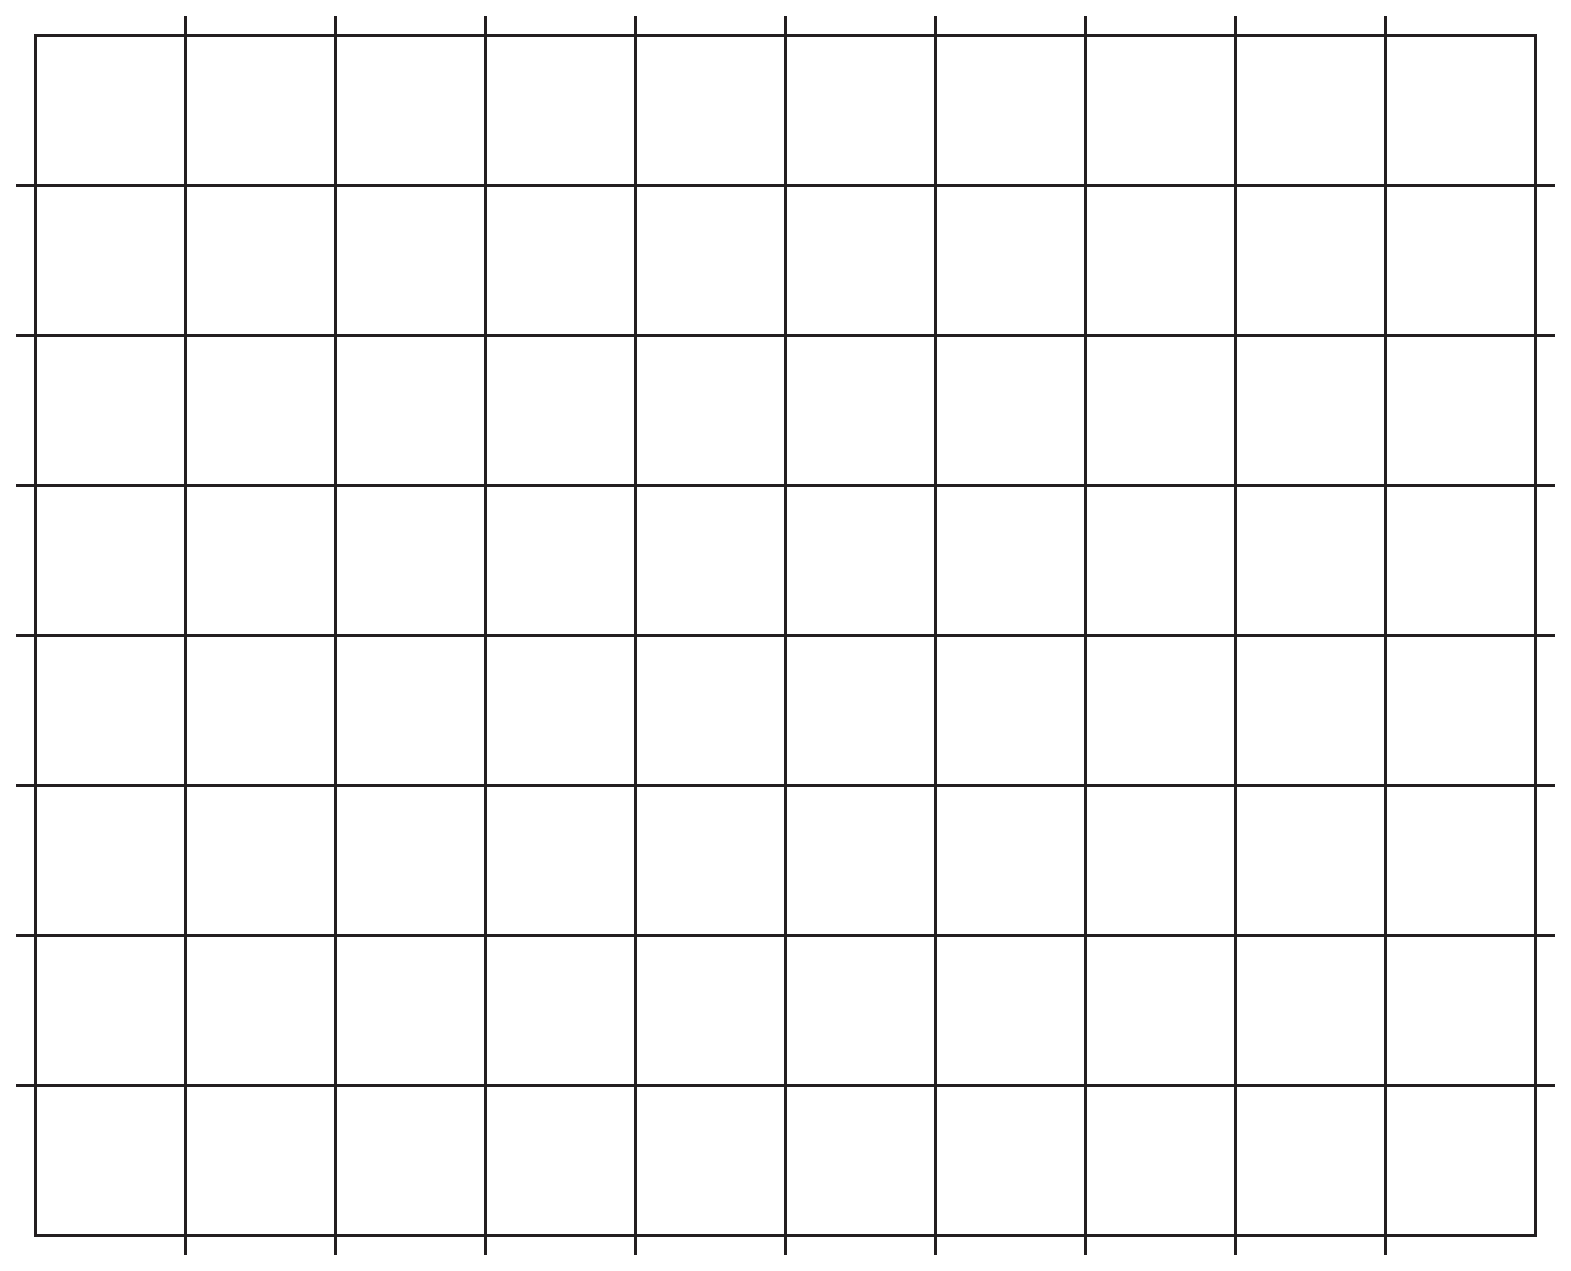
\includegraphics[keepaspectratio, scale=0.28, angle=0]
                  {figs/eps/grid.eps}
                  %\caption{オシロスコープの画面スケッチ}
                  \label{fig:grid50mV}
  \end{figure}

  \begin{spacing}{1.5}
  \begin{tabular}{|c||r|r|r|}
    \multicolumn{4}{c}{入力(実効値)$V_i=50\;$mVの時の出力} \\ \hline
    項目 & DIVs & Value/DIV & Value \\ \hline \hline
    振幅pp &      & 5.0[V]&      \\ \hline
    波長 &      & 200.0[$\mu$s]&      \\ \hline
  \end{tabular}
\end{spacing}
\end{multicols}

\vfill
\newpage

\subsection{周波数特性を測定する}

周波数特性(オシロスコープで出力波形を観察、記録する)

\begin{enumerate}
\item[(1)] 電源電圧を$E_C(V_{CC})=12$Vとし、入力電圧を$V_i=5m$V 一定の正弦波とする
\item[(2)] 入力の周波数を変えて、その都度出力電圧$V_o$を記録する($V_i=5m$V を一定を保つ)
\item[(3)] 電圧増幅度$A_v=V_o/V_i$、および電圧利得$G_v[dB]=20\log A_v$を計算する
\item[(4)] 周波数特性(周波数ー電圧利得)を、周波数を対数とする片対数グラフに表す
\item[(5)] 中域周波数での電圧利得$G_{vA}$を読み取り、そこから$3dB$低下した増幅度$G_{vA}-3$を求める
\item[(6)] 低域遮断周波数$f_L$、高域遮断周波数$f_H$、帯域幅$B$をグラフから読み取る
\end{enumerate}

%\begin{spacing}{0.67}
%  \begin{multicols}{2}
\begin{figure}[H]
  \centering
   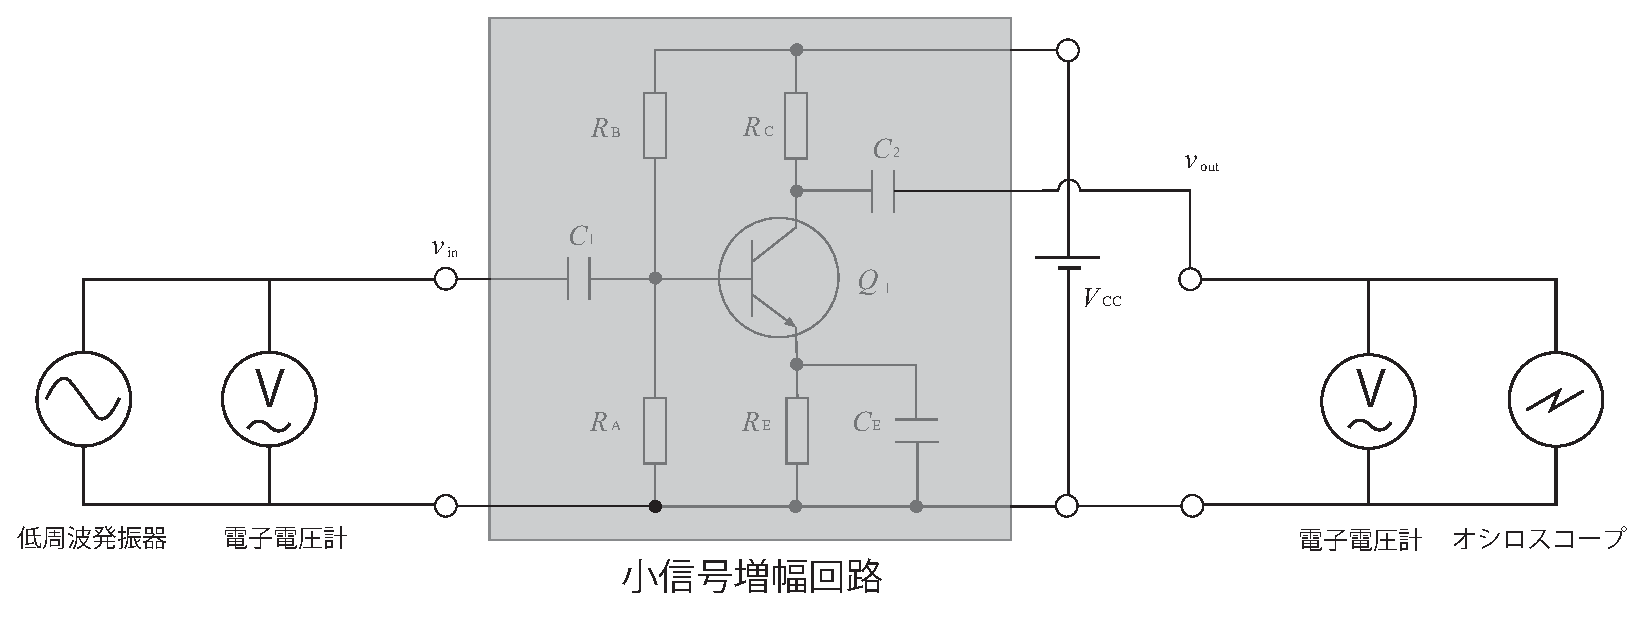
\includegraphics[keepaspectratio, scale=0.48, angle=0]
             {figs/eps/exp0.eps}
             \caption{実習装置}
             \label{fig:exp0}
\end{figure}

%周波数特性のグラフ作図例

\begin{figure}[H]
    \centering
     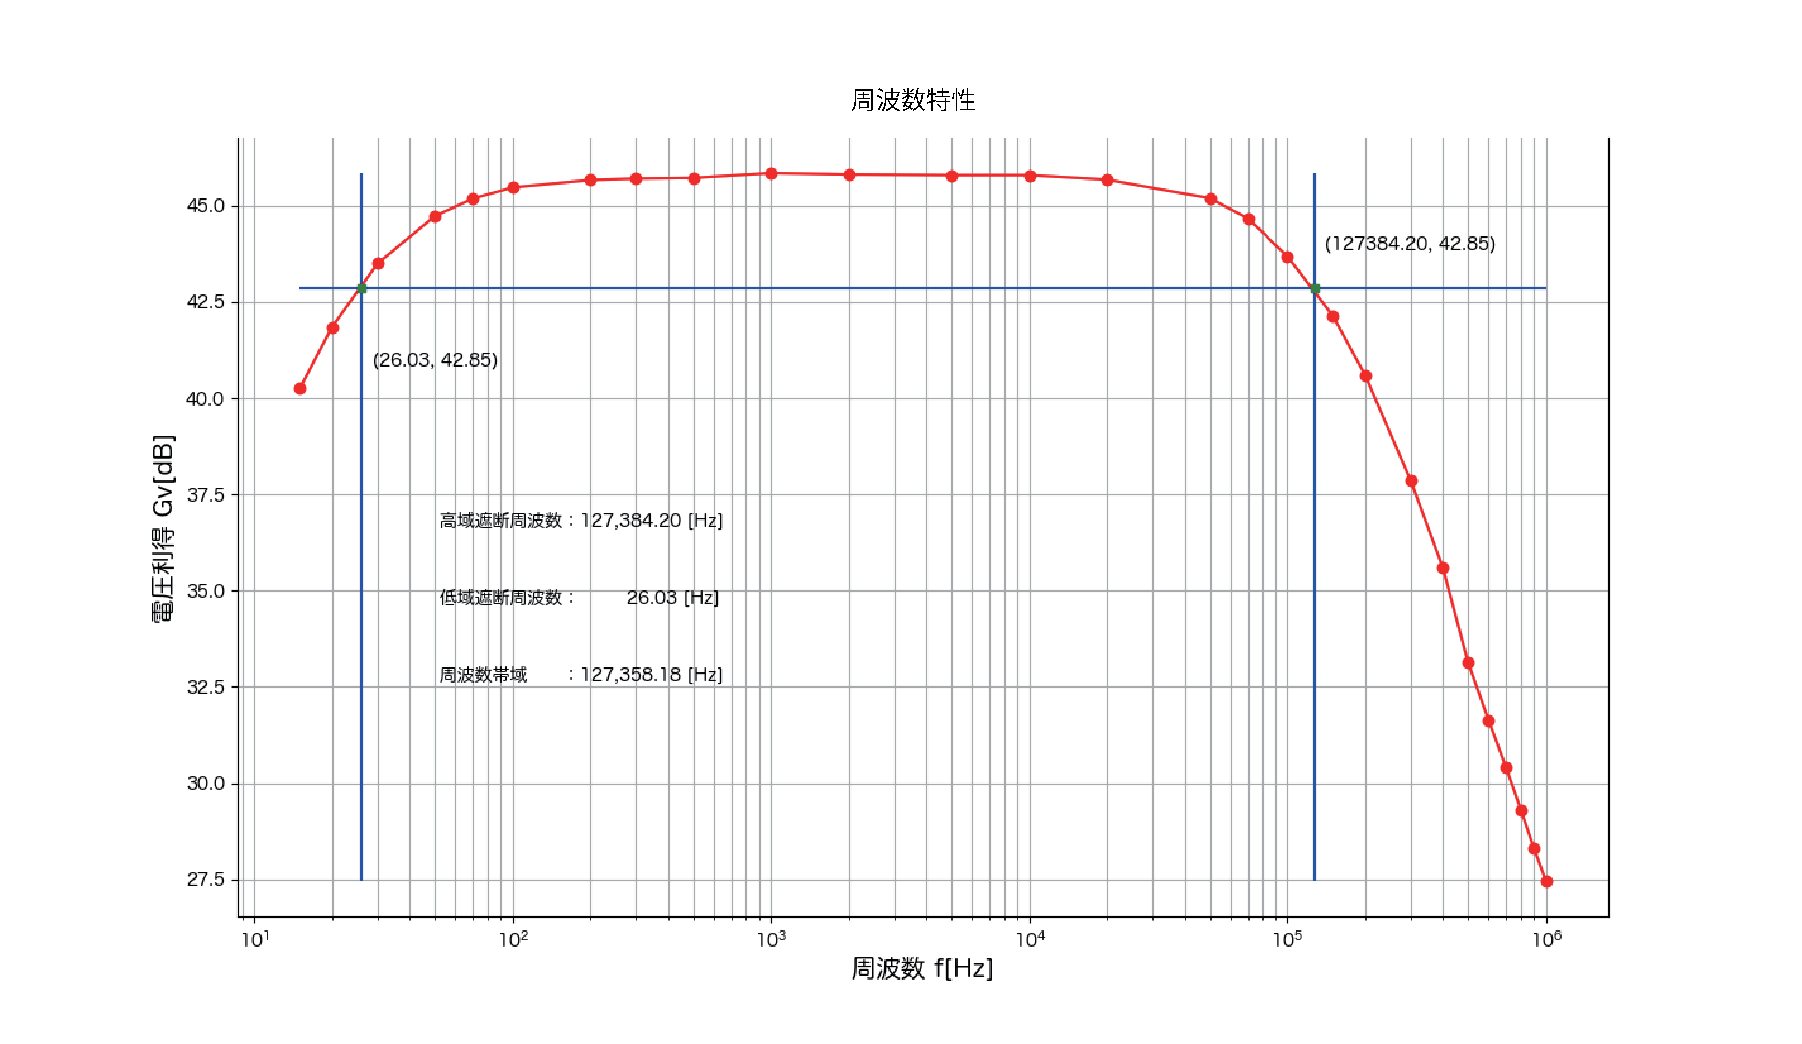
\includegraphics[keepaspectratio, scale=0.55, angle=0]
               {figs/eps/freqcharM1YExample.eps}
               \caption{周波数特性のグラフ作成例}
               \label{fig:freqcharM1Yd}
\end{figure}
%  \end{multicols}
%\end{spacing}

\newpage

\begin{figure}[H]
  \centering
   \includegraphics[keepaspectratio, scale=0.76, angle=90]
               {figs/eps/kiroku.eps}
               \caption{周波数特性の記録用紙}
               \label{fig:22_2}
\end{figure}

\newpage

【周波数特性:オシロスコープ画面の情報をスケッチせよ】

\begin{multicols}{2}
  \begin{figure}[H]
     \centering
      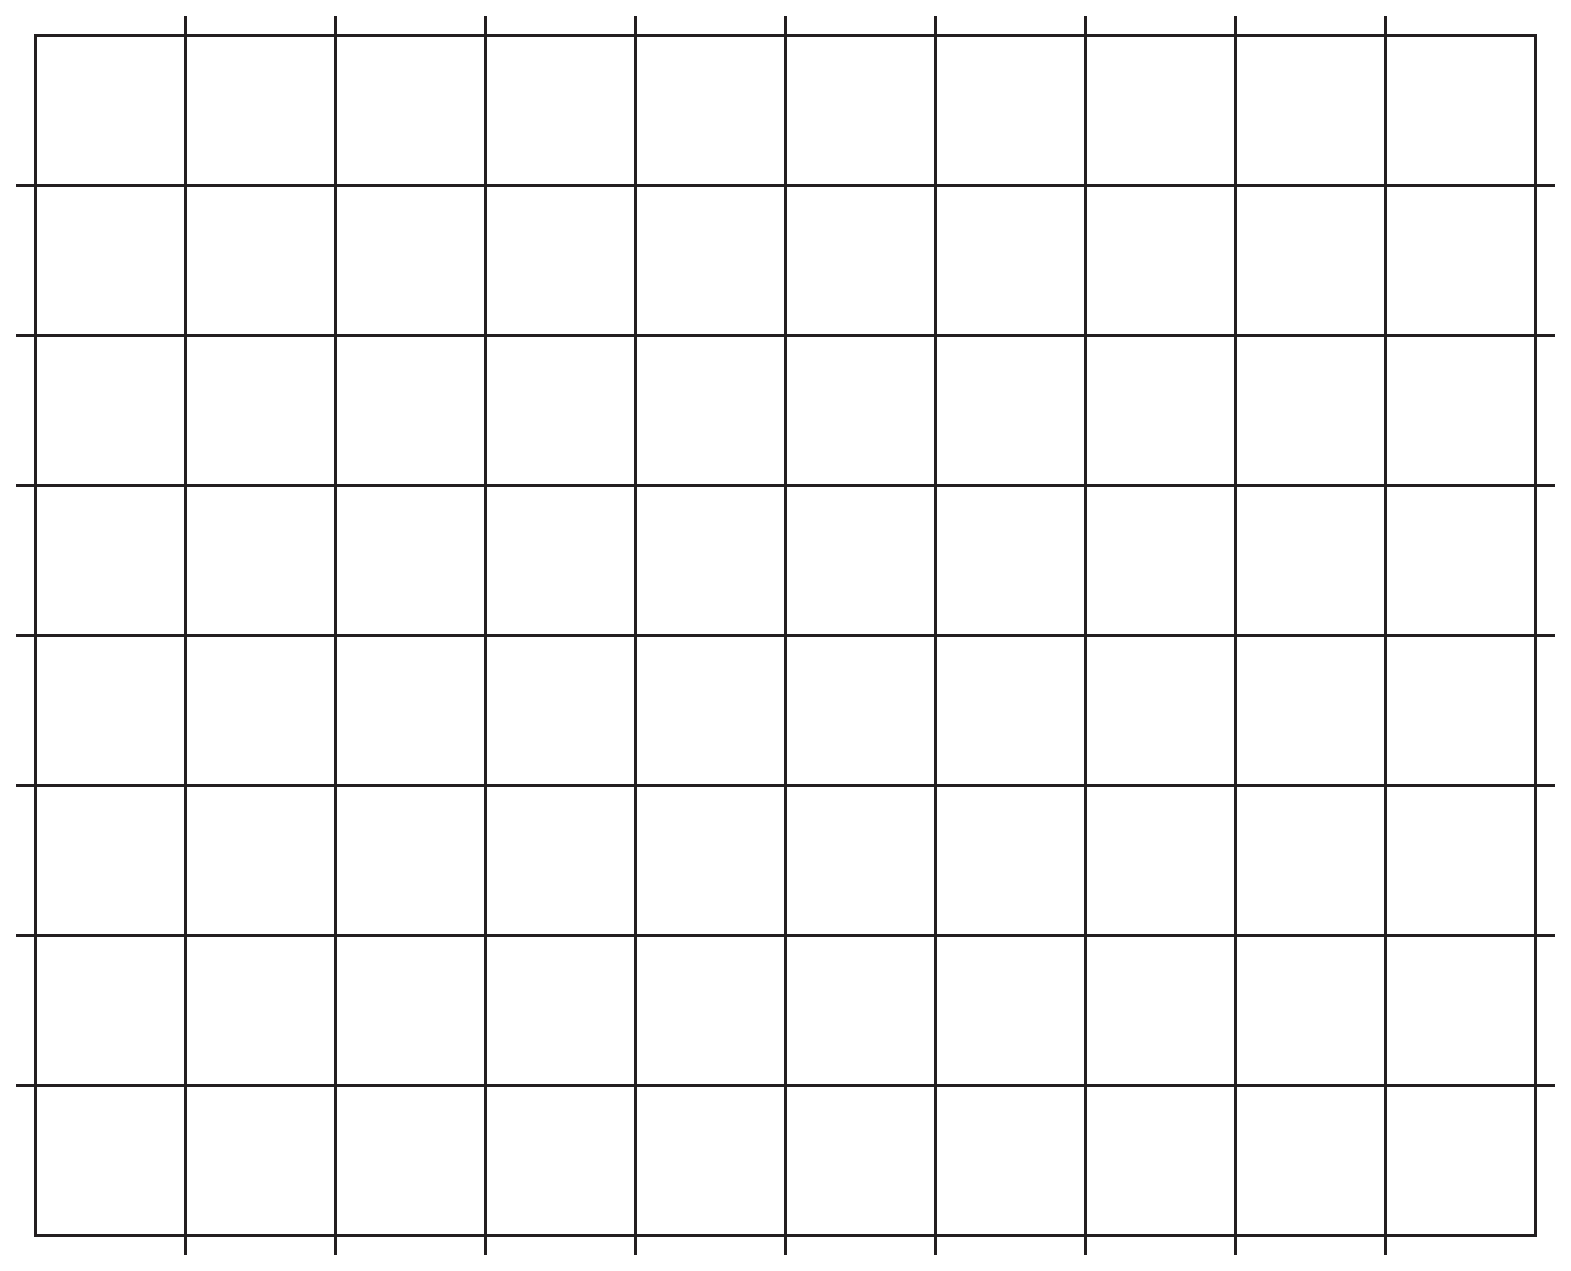
\includegraphics[keepaspectratio, scale=0.28, angle=0]
                  {figs/eps/grid.eps}
                  %\caption{オシロスコープの画面スケッチ}
                  \label{fig:grid6mV}
  \end{figure}

  \begin{spacing}{1.5}
  \begin{tabular}{|c||r|r|r|}
    \multicolumn{4}{c}{入力周波数 $f=15Hz\;$ の時の出力} \\ \hline
    項目 & DIVs & Value/DIV & Value \\ \hline \hline
    振幅pp &      & 500[mV]&      \\ \hline
    波長 &      & 20.0[ms]&      \\ \hline
  \end{tabular}
\end{spacing}
\end{multicols}

\vfill

\begin{multicols}{2}
  \begin{figure}[H]
     \centering
      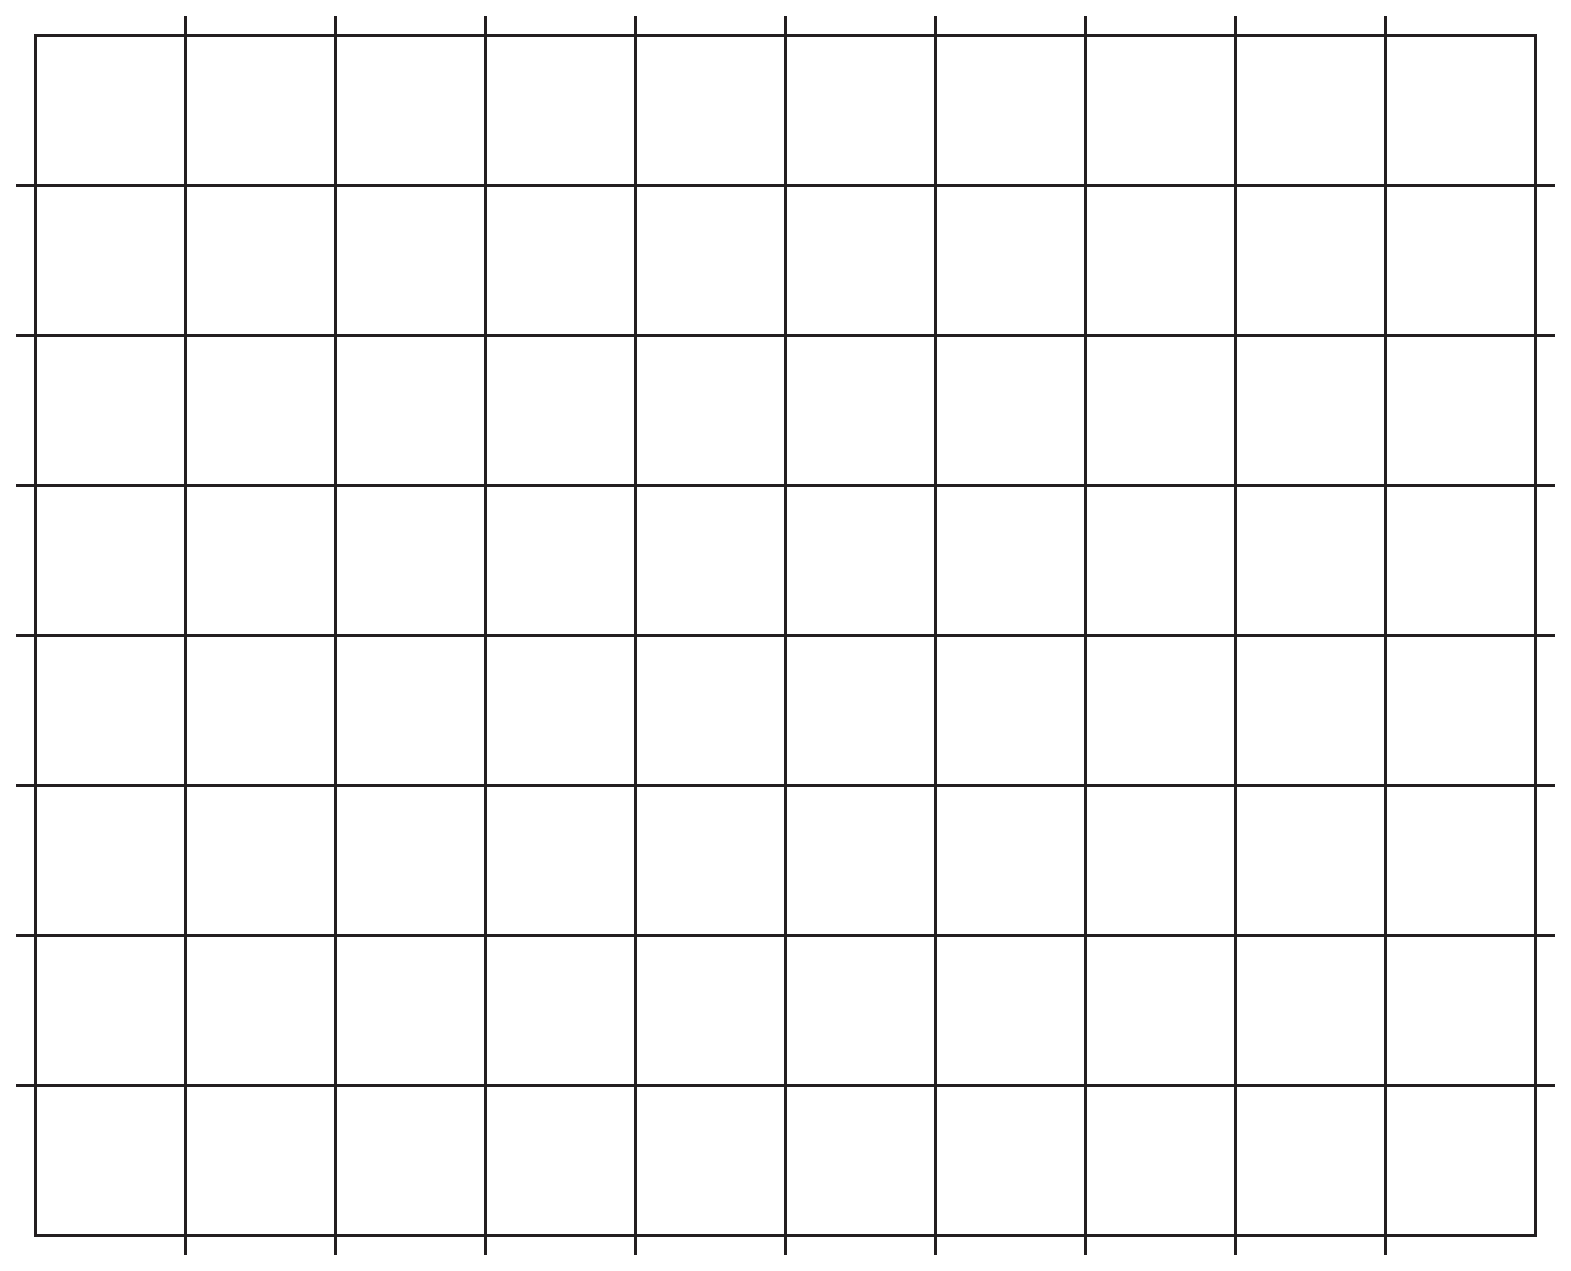
\includegraphics[keepaspectratio, scale=0.28, angle=0]
                  {figs/eps/grid.eps}
                  %\caption{オシロスコープの画面スケッチ}
                  \label{fig:grid10mV}
  \end{figure}

  \begin{spacing}{1.5}
  \begin{tabular}{|c||r|r|r|}
    \multicolumn{4}{c}{入力周波数 $f=20Hz\;$ の時の出力} \\ \hline
    項目 & DIVs & Value/DIV & Value \\ \hline \hline
    振幅pp &      & 500[mV]&      \\ \hline
    波長 &      & 20.0[ms]&      \\ \hline
  \end{tabular}
\end{spacing}
\end{multicols}

\vfill

\begin{multicols}{2}
  \begin{figure}[H]
     \centering
      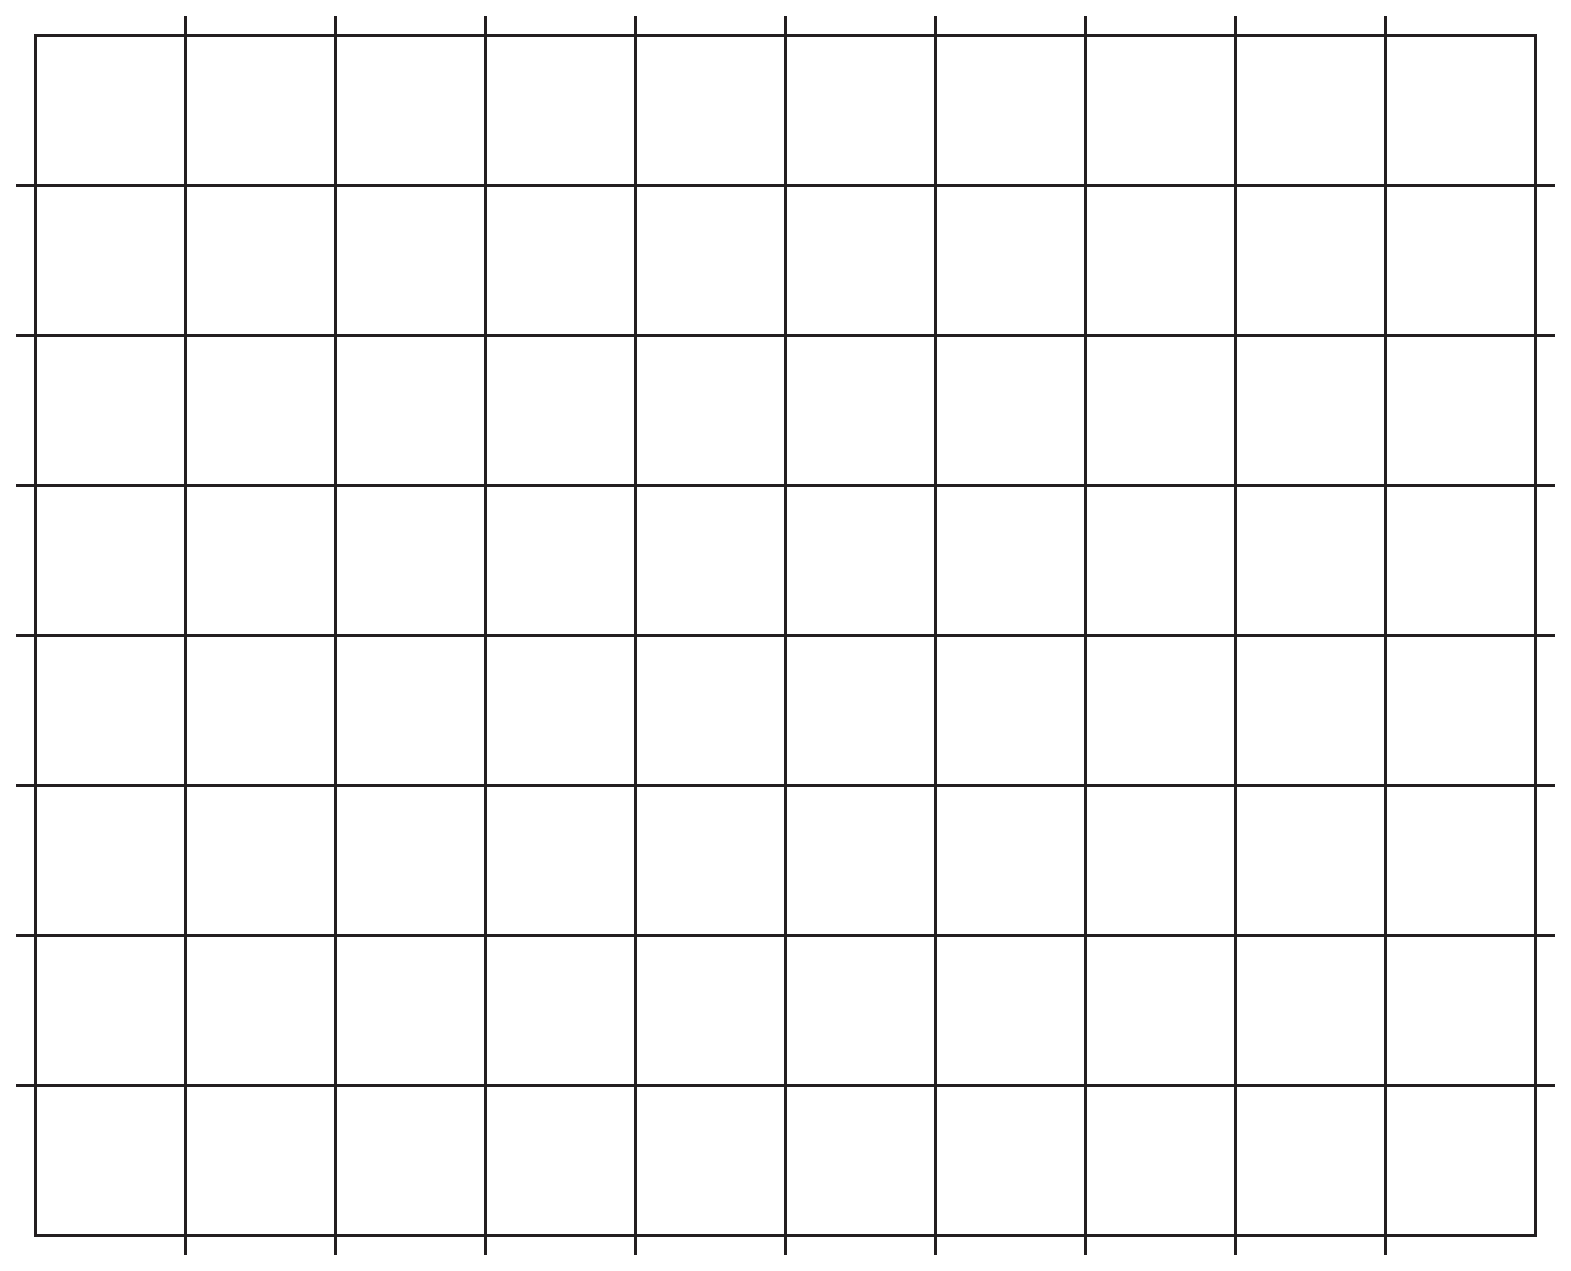
\includegraphics[keepaspectratio, scale=0.28, angle=0]
                  {figs/eps/grid.eps}
                  %\caption{オシロスコープの画面スケッチ}
                  \label{fig:grid20mV}
  \end{figure}

  \begin{spacing}{1.5}
  \begin{tabular}{|c||r|r|r|}
    \multicolumn{4}{c}{入力周波数 $f=30Hz\;$ の時の出力} \\ \hline
    項目 & DIVs & Value/DIV & Value \\ \hline \hline
    振幅pp &      & 500[mV]&      \\ \hline
    波長 &      & 20.0[ms]&      \\ \hline
  \end{tabular}
\end{spacing}
\end{multicols}

\vfill

\newpage

\begin{multicols}{2}
  \begin{figure}[H]
     \centering
      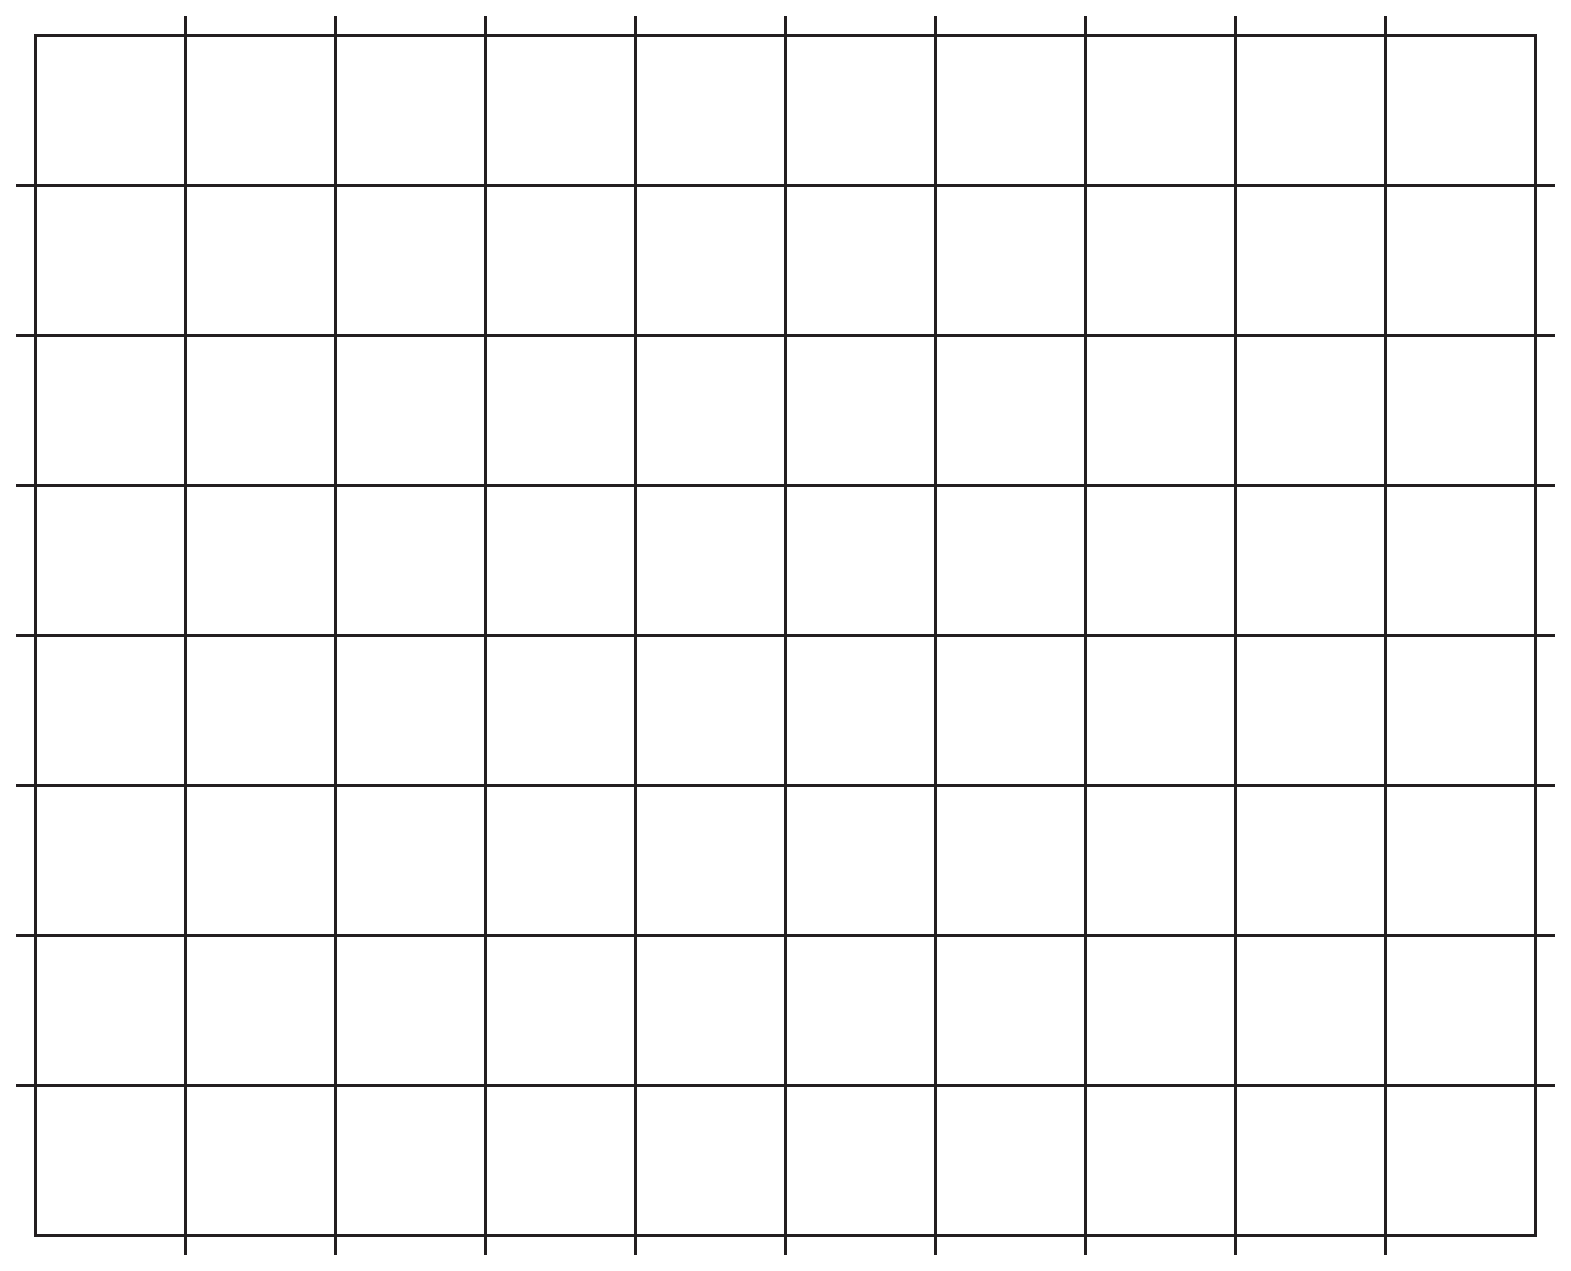
\includegraphics[keepaspectratio, scale=0.28, angle=0]
                  {figs/eps/grid.eps}
                  %\caption{オシロスコープの画面スケッチ}
                  \label{fig:grid30mV}
  \end{figure}

  \begin{spacing}{1.5}
  \begin{tabular}{|c||r|r|r|}
    \multicolumn{4}{c}{入力周波数 $f=50Hz\;$ の時の出力} \\ \hline
    項目 & DIVs & Value/DIV & Value \\ \hline \hline
    振幅pp &      & 500[mV]&      \\ \hline
    波長 &      & 10[ms]&      \\ \hline
  \end{tabular}
\end{spacing}
\end{multicols}

\vfill

\begin{multicols}{2}
  \begin{figure}[H]
     \centering
      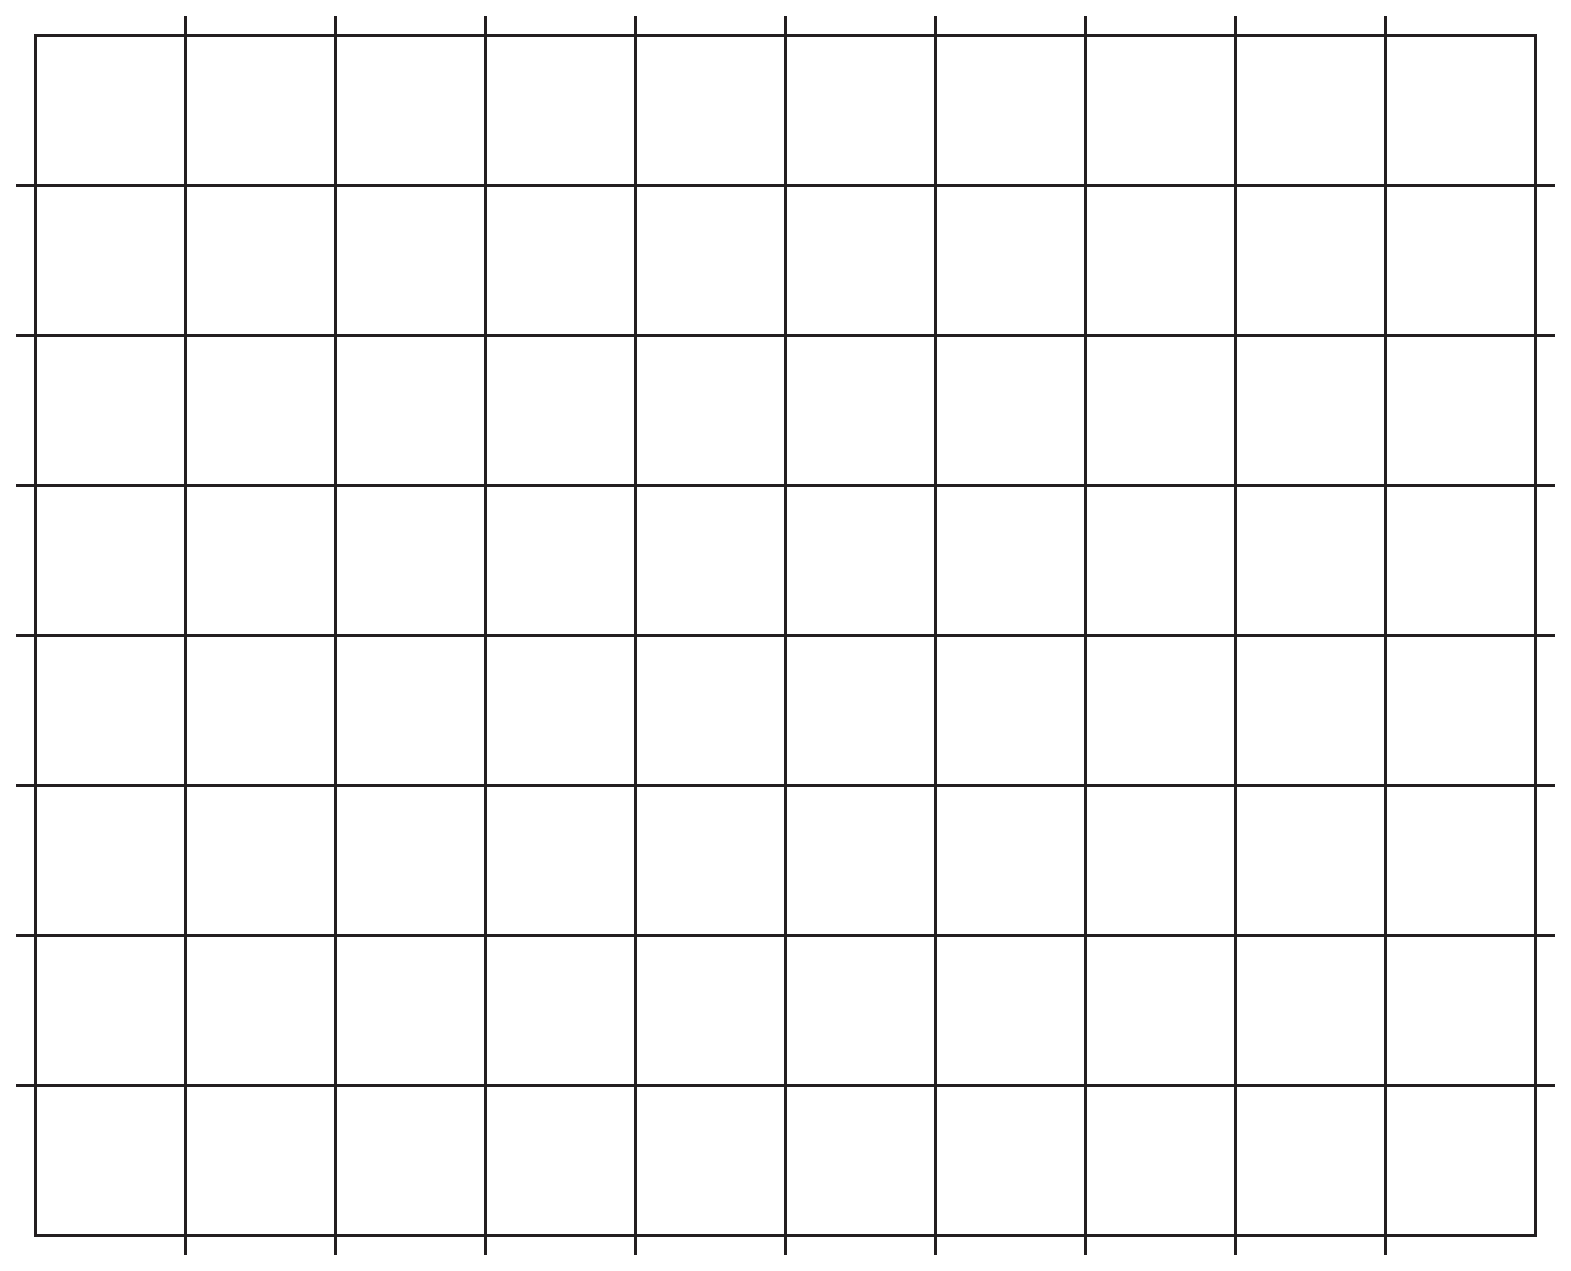
\includegraphics[keepaspectratio, scale=0.28, angle=0]
                  {figs/eps/grid.eps}
                  %\caption{オシロスコープの画面スケッチ}
                  \label{fig:grid40mV}
  \end{figure}

  \begin{spacing}{1.5}
  \begin{tabular}{|c||r|r|r|}
    \multicolumn{4}{c}{入力周波数 $f=70Hz\;$ の時の出力} \\ \hline
    項目 & DIVs & Value/DIV & Value \\ \hline \hline
    振幅pp &      & 500[mV]&      \\ \hline
    波長 &      & 5[ms]&      \\ \hline
  \end{tabular}
\end{spacing}
\end{multicols}

\vfill

\begin{multicols}{2}
  \begin{figure}[H]
     \centering
      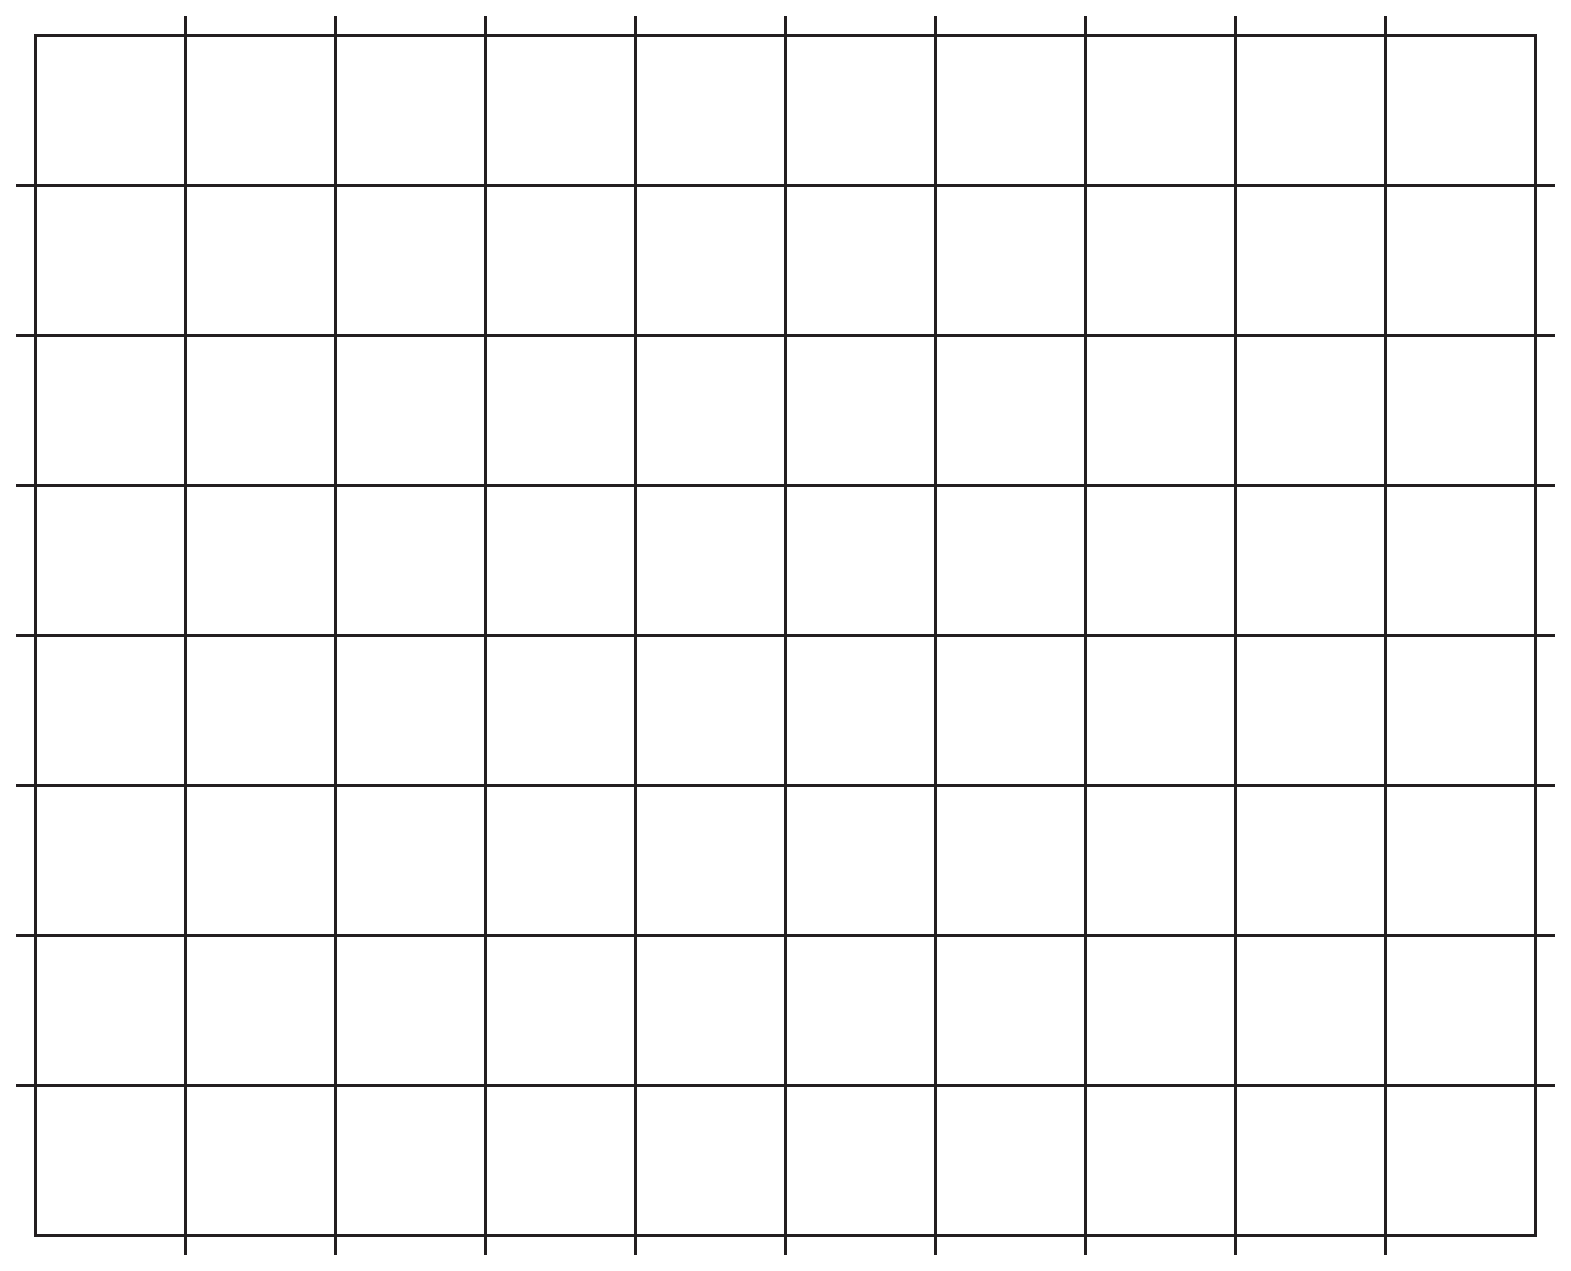
\includegraphics[keepaspectratio, scale=0.28, angle=0]
                  {figs/eps/grid.eps}
                  %\caption{オシロスコープの画面スケッチ}
                  \label{fig:grid50mV}
  \end{figure}

  \begin{spacing}{1.5}
  \begin{tabular}{|c||r|r|r|}
    \multicolumn{4}{c}{入力周波数 $f=100Hz\;$ の時の出力} \\ \hline
    項目 & DIVs & Value/DIV & Value \\ \hline \hline
    振幅pp &      & 500[mV]&      \\ \hline
    波長 &      & 5.0[ms]&      \\ \hline
  \end{tabular}
\end{spacing}
\end{multicols}

\vfill

\newpage

\begin{multicols}{2}
  \begin{figure}[H]
     \centering
      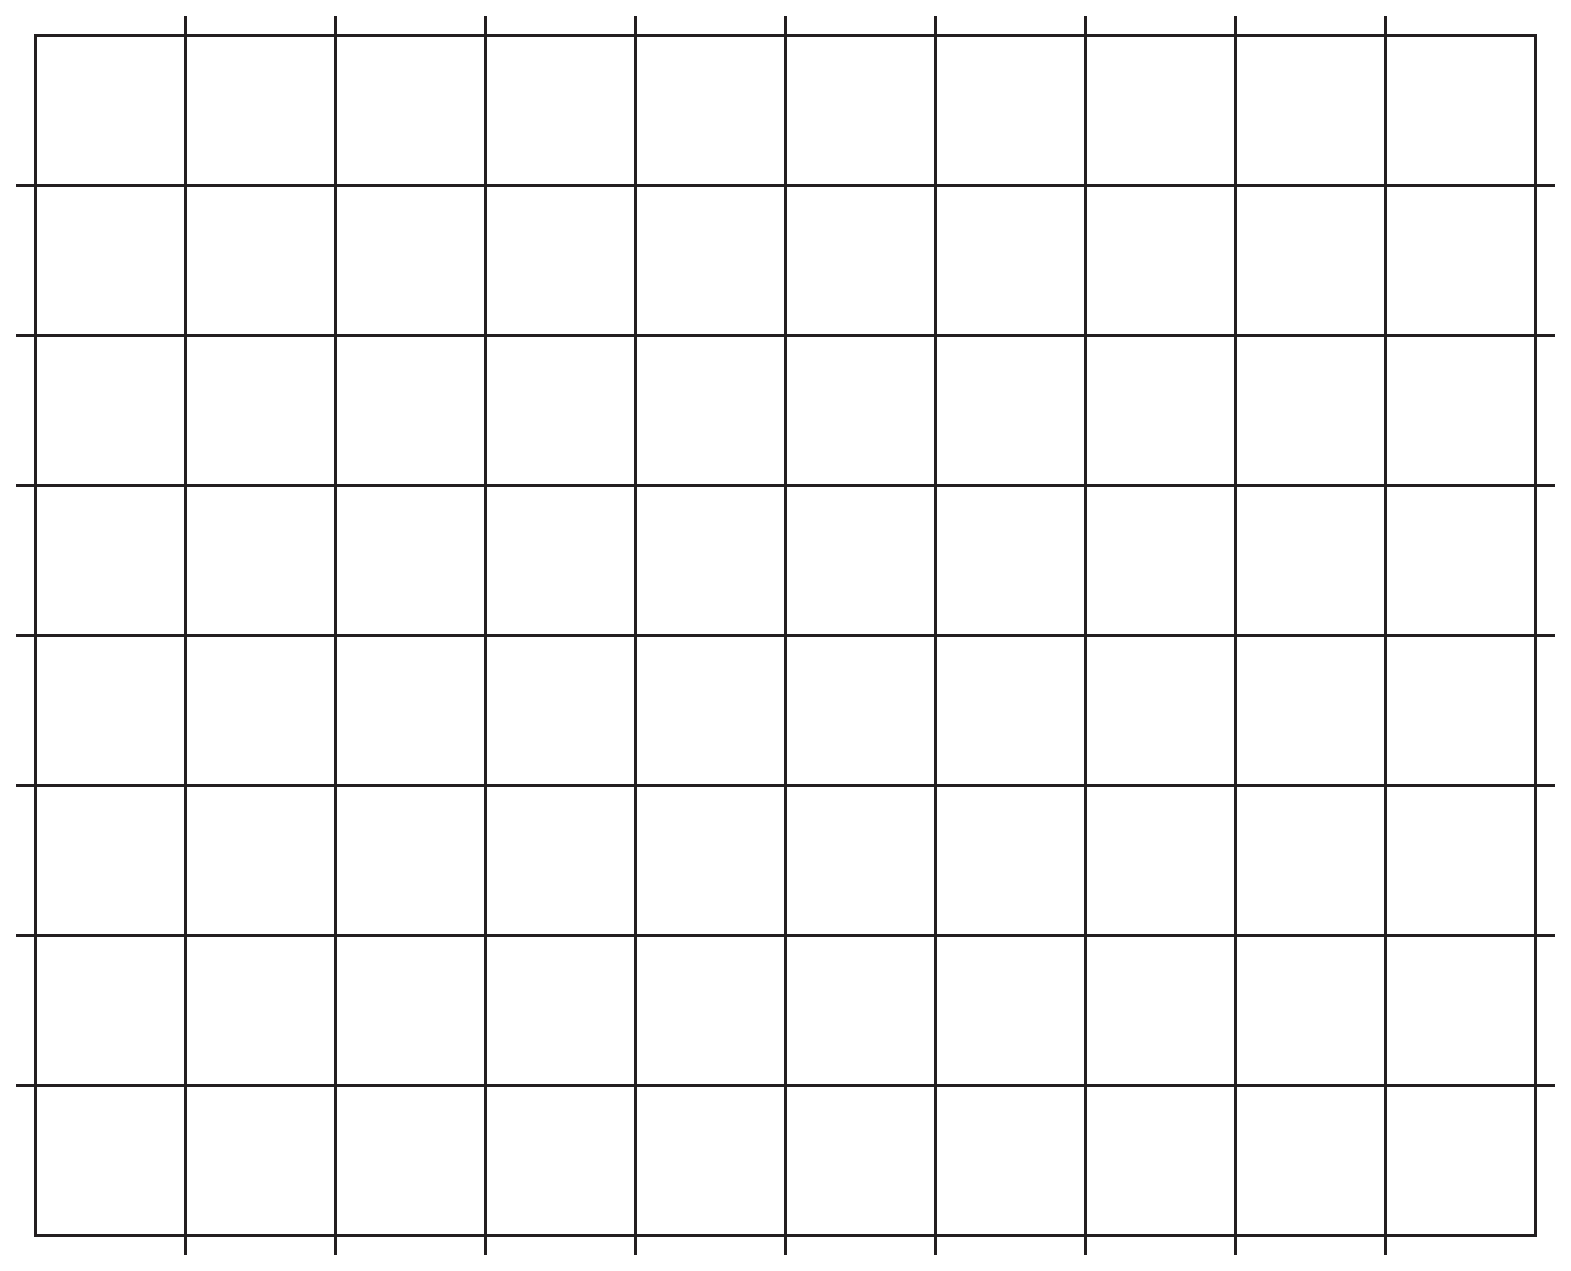
\includegraphics[keepaspectratio, scale=0.28, angle=0]
                  {figs/eps/grid.eps}
                  %\caption{オシロスコープの画面スケッチ}
                  \label{fig:grid30mV}
  \end{figure}

  \begin{spacing}{1.5}
  \begin{tabular}{|c||r|r|r|}
    \multicolumn{4}{c}{入力周波数 $f=1kHz\;$ の時の出力} \\ \hline
    項目 & DIVs & Value/DIV & Value \\ \hline \hline
    振幅pp &      & 500[mV]&      \\ \hline
    波長 &      & 200[$\mu$s]&      \\ \hline
  \end{tabular}
\end{spacing}
\end{multicols}

\vfill

\begin{multicols}{2}
  \begin{figure}[H]
     \centering
      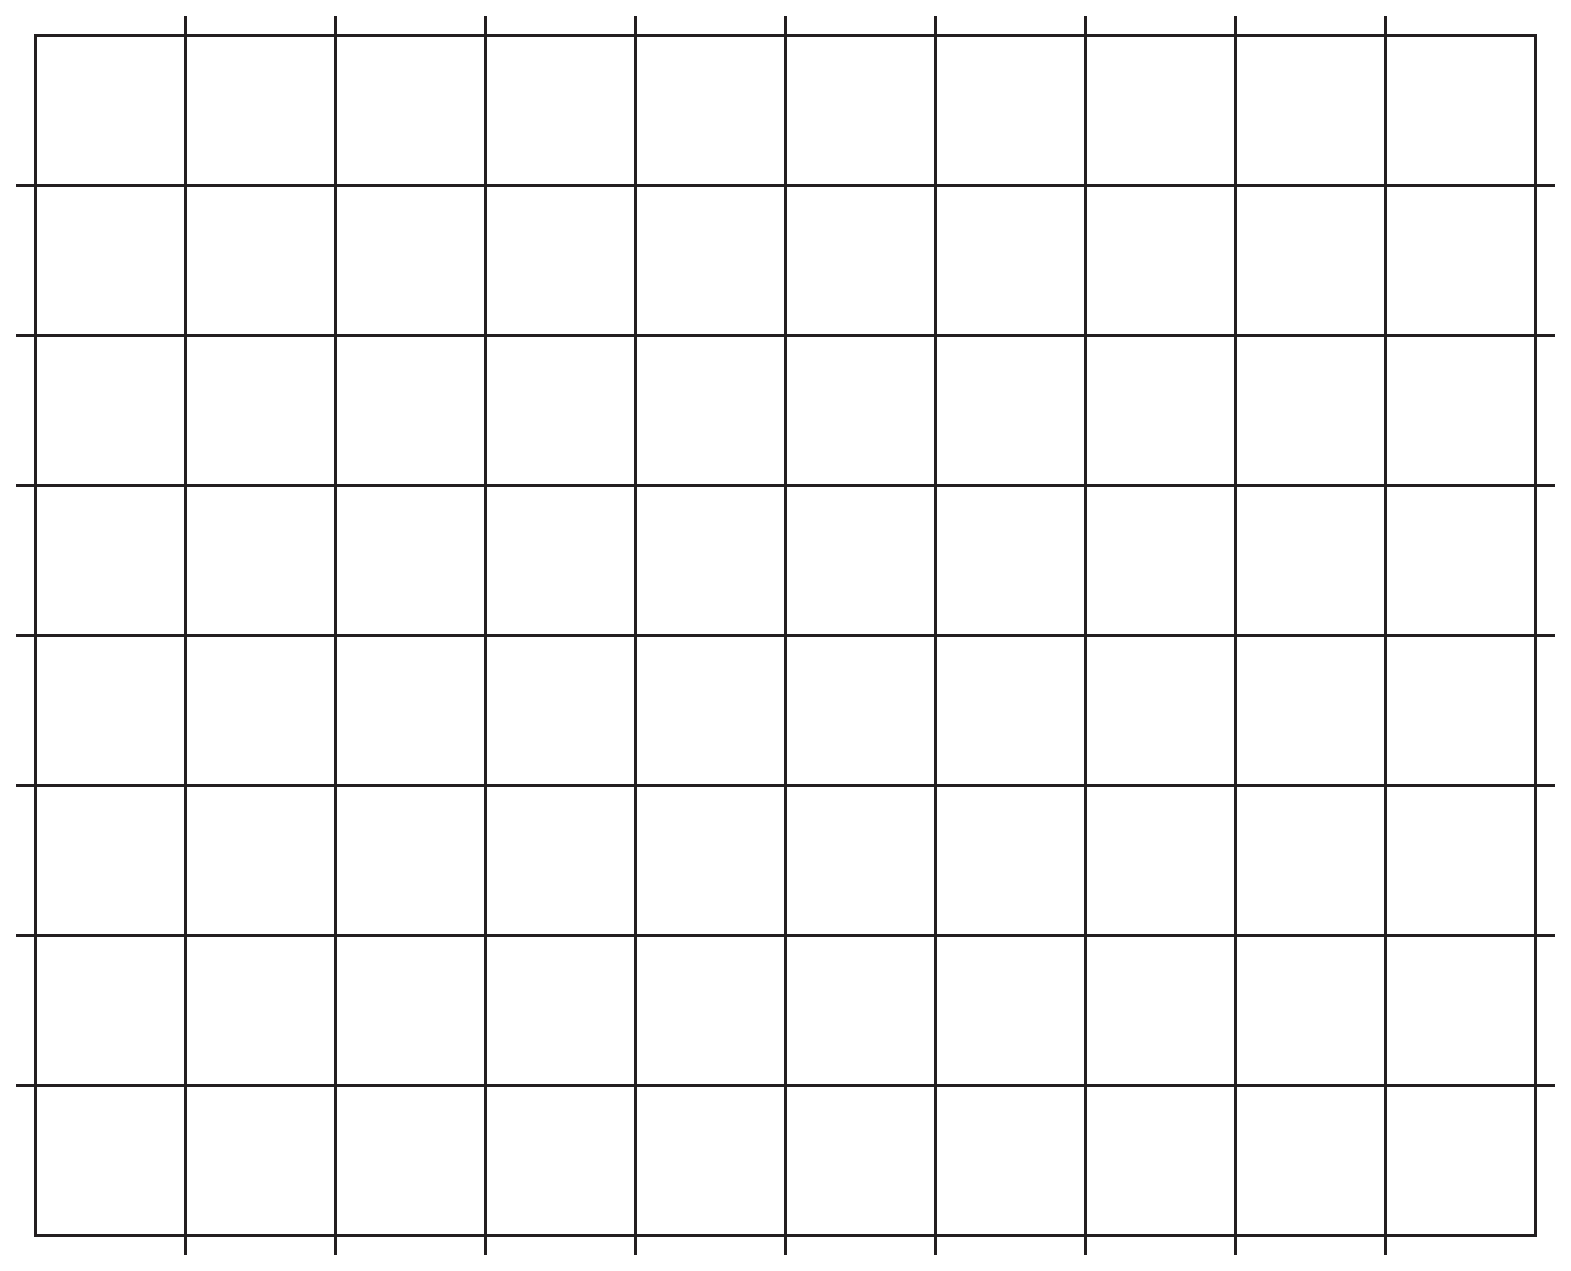
\includegraphics[keepaspectratio, scale=0.28, angle=0]
                  {figs/eps/grid.eps}
                  %\caption{オシロスコープの画面スケッチ}
                  \label{fig:grid40mV}
  \end{figure}

  \begin{spacing}{1.5}
  \begin{tabular}{|c||r|r|r|}
    \multicolumn{4}{c}{入力周波数 $f=10kHz\;$ の時の出力} \\ \hline
    項目 & DIVs & Value/DIV & Value \\ \hline \hline
    振幅pp &      & 500[mV]&      \\ \hline
    波長 &      & 20,0[$\mu$s]&      \\ \hline
  \end{tabular}
\end{spacing}
\end{multicols}

\vfill

\begin{multicols}{2}
  \begin{figure}[H]
     \centering
      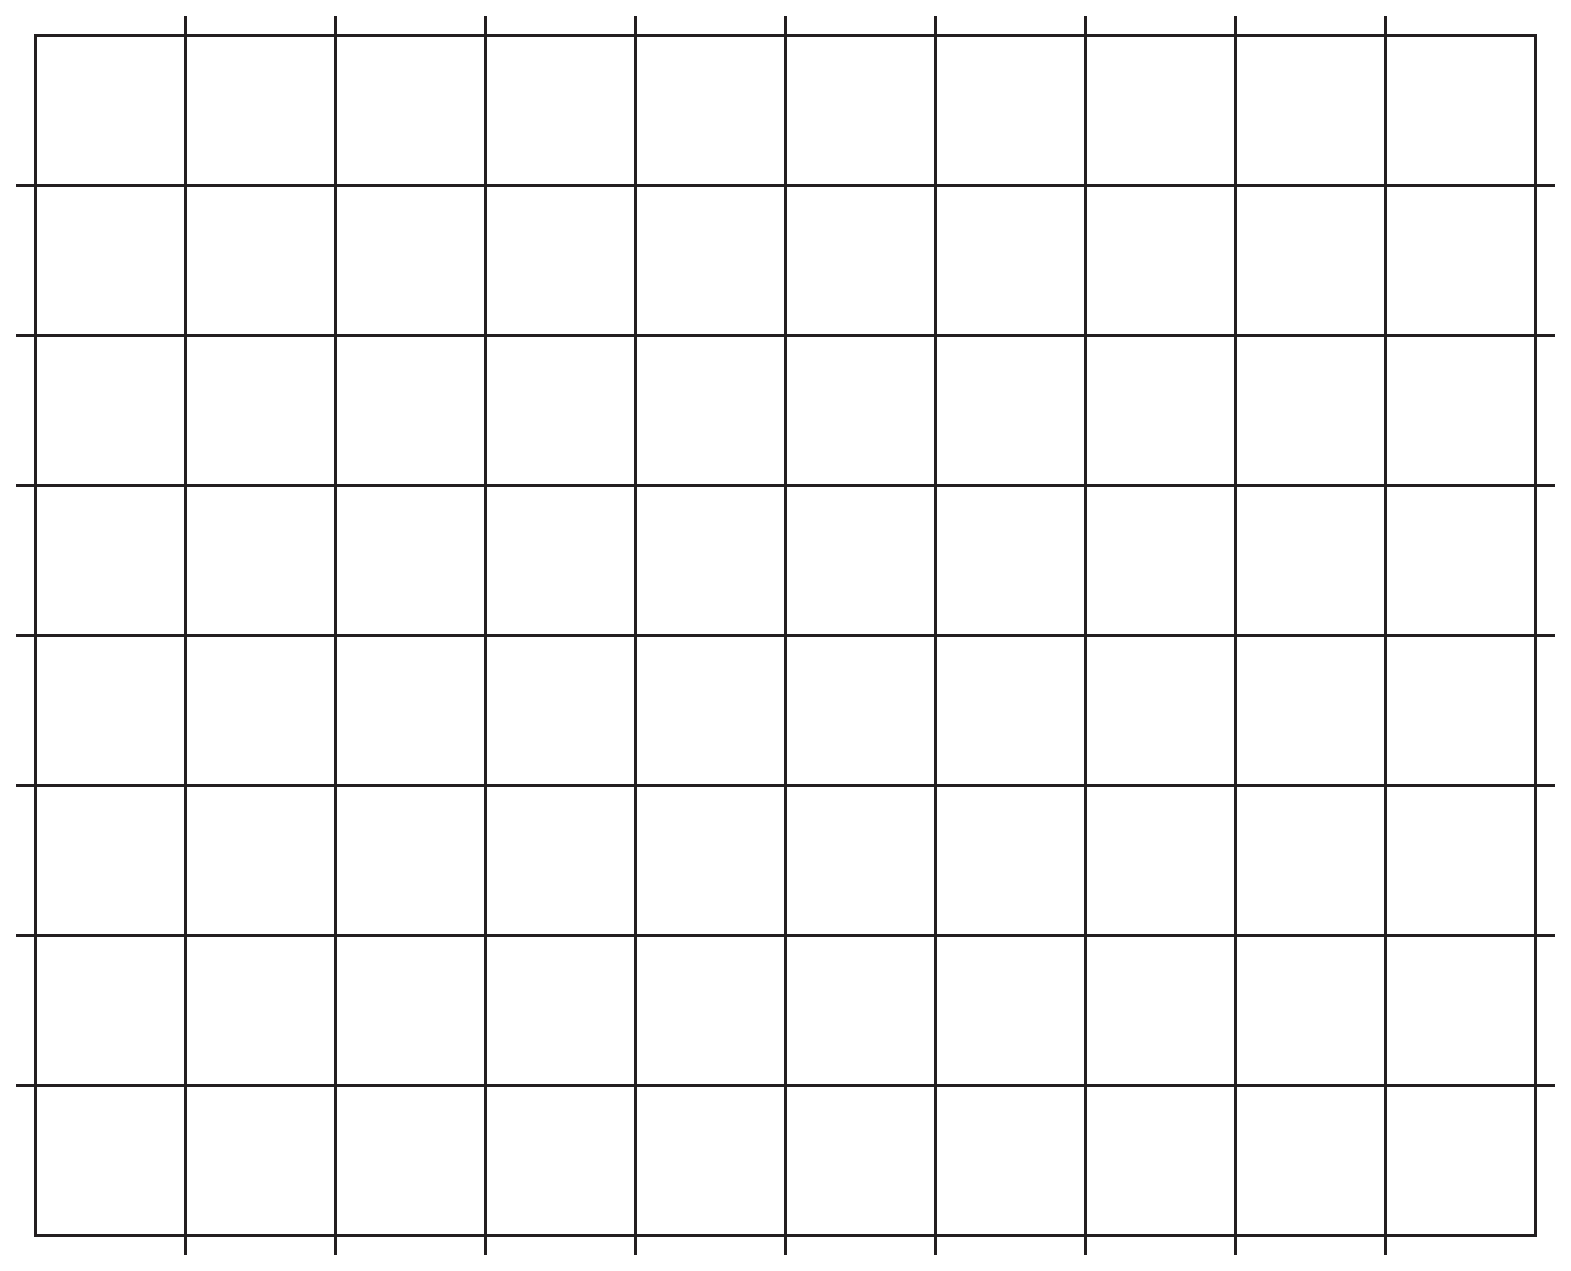
\includegraphics[keepaspectratio, scale=0.28, angle=0]
                  {figs/eps/grid.eps}
                  %\caption{オシロスコープの画面スケッチ}
                  \label{fig:grid50mV}
  \end{figure}

  \begin{spacing}{1.5}
  \begin{tabular}{|c||r|r|r|}
    \multicolumn{4}{c}{入力周波数 $f=100kHz\;$ の時の出力} \\ \hline
    項目 & DIVs & Value/DIV & Value \\ \hline \hline
    振幅pp &      & 500[mV]&      \\ \hline
    波長 &      & 2.00[$\mu$s]&      \\ \hline
  \end{tabular}
\end{spacing}
\end{multicols}

\vfill

\newpage

\begin{multicols}{2}
  \begin{figure}[H]
     \centering
      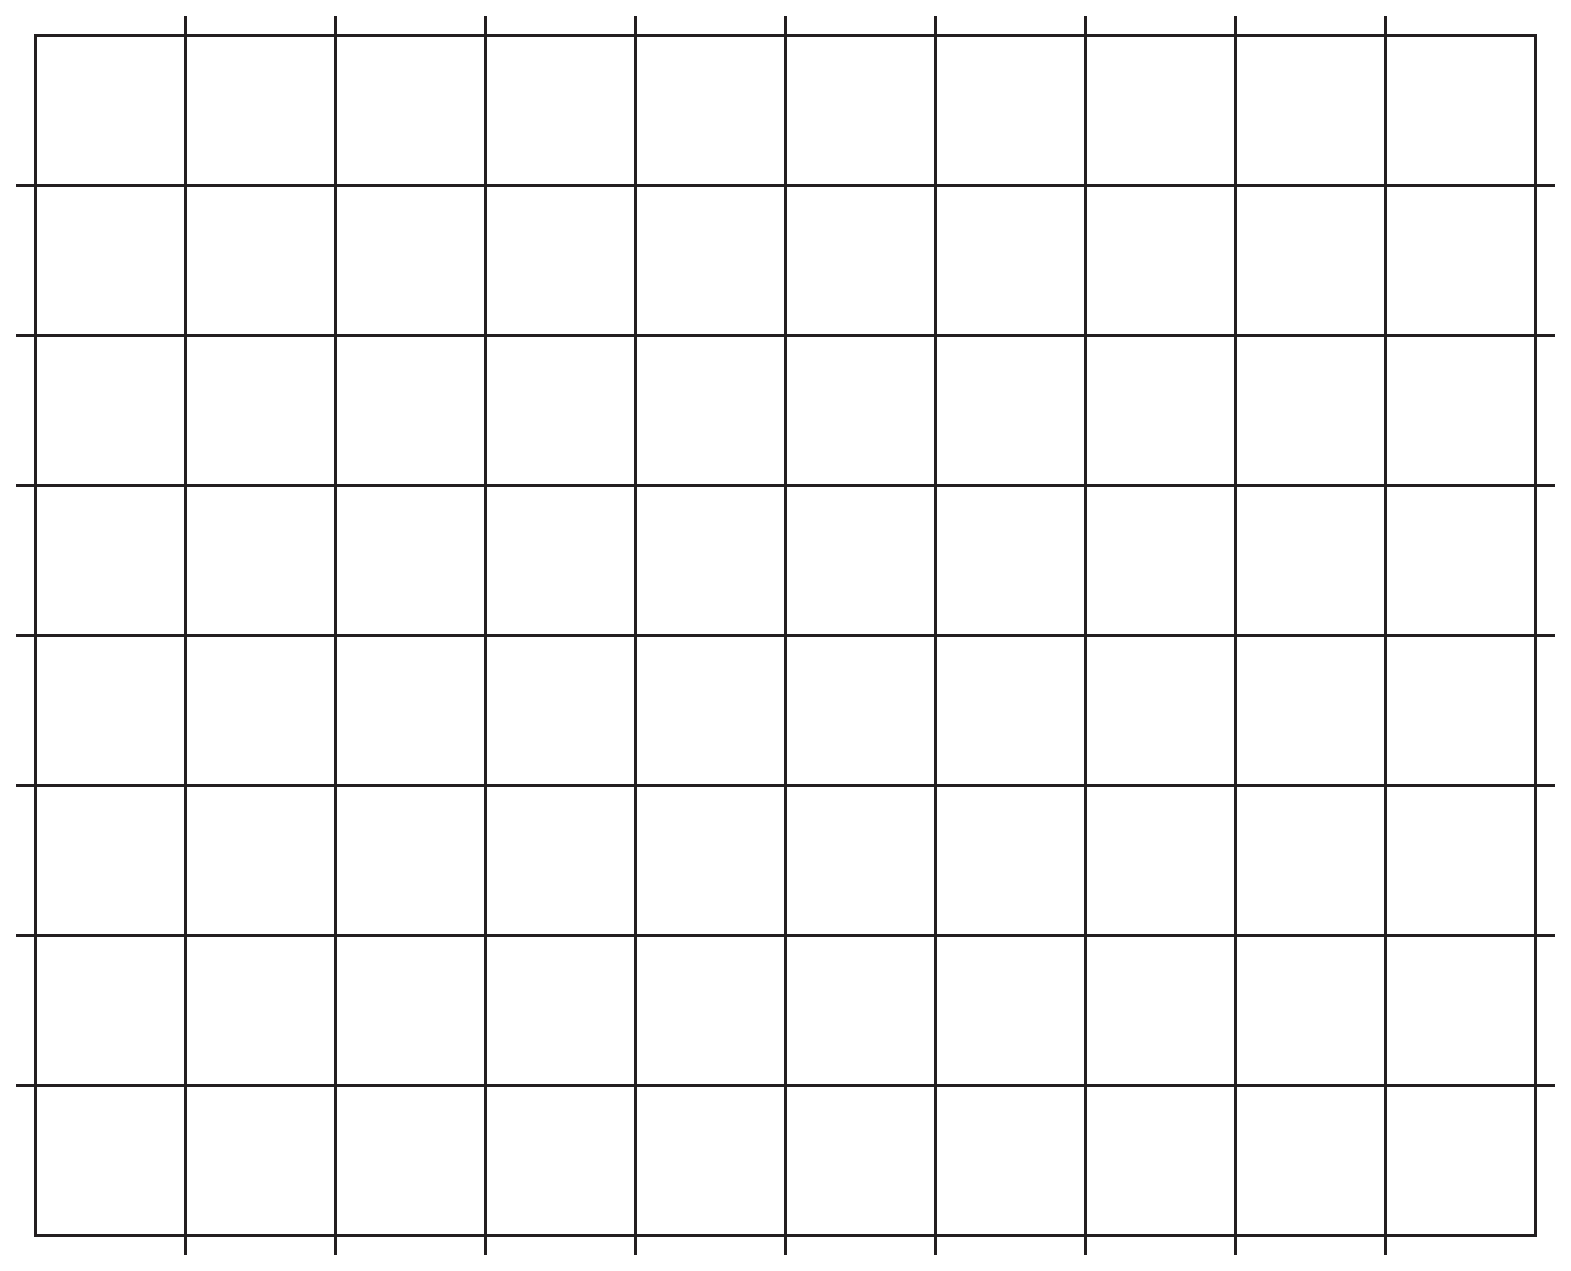
\includegraphics[keepaspectratio, scale=0.28, angle=0]
                  {figs/eps/grid.eps}
                  %\caption{オシロスコープの画面スケッチ}
                  \label{fig:grid30mV}
  \end{figure}

  \begin{spacing}{1.5}
  \begin{tabular}{|c||r|r|r|}
    \multicolumn{4}{c}{入力周波数 $f=400kHz\;$ の時の出力} \\ \hline
    項目 & DIVs & Value/DIV & Value \\ \hline \hline
    振幅pp &      & 500[mV]&      \\ \hline
    波長 &      & 1.00[$\mu$s]&      \\ \hline
  \end{tabular}
\end{spacing}
\end{multicols}

\vfill

\begin{multicols}{2}
  \begin{figure}[H]
     \centering
      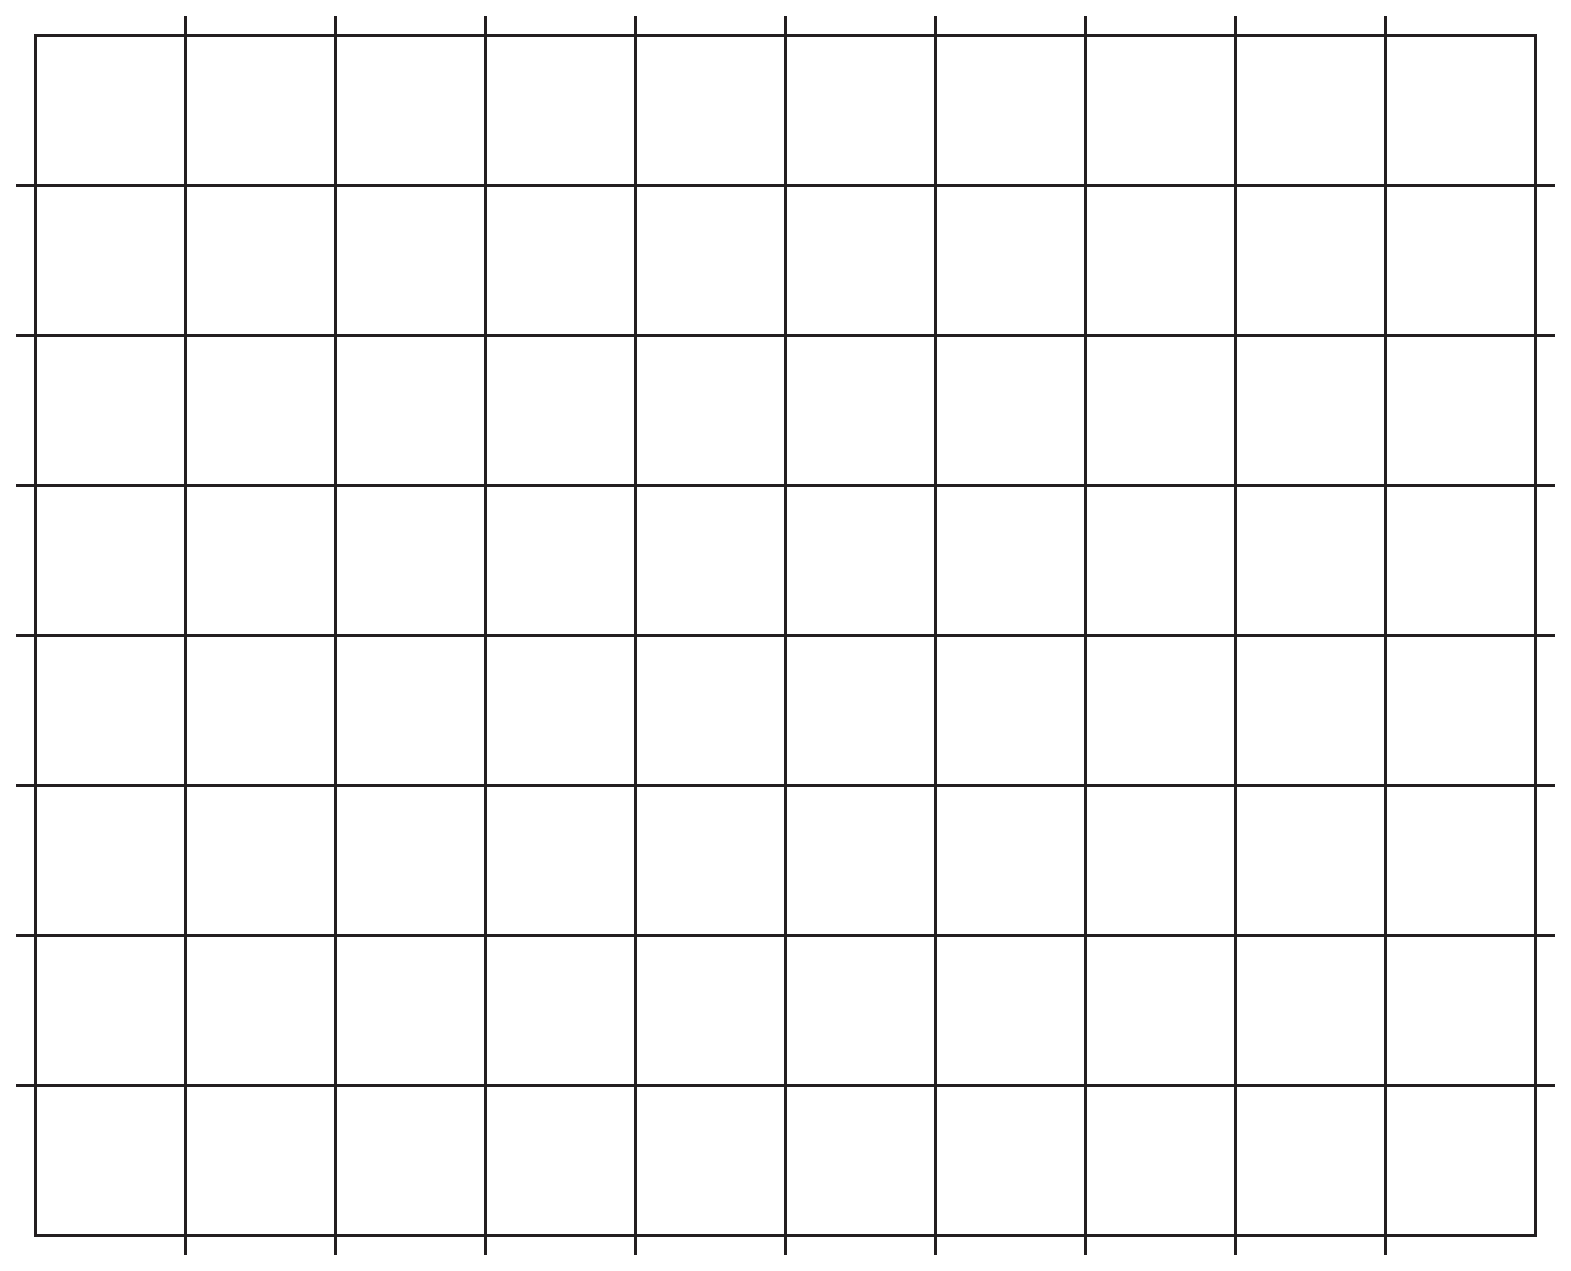
\includegraphics[keepaspectratio, scale=0.28, angle=0]
                  {figs/eps/grid.eps}
                  %\caption{オシロスコープの画面スケッチ}
                  \label{fig:grid40mV}
  \end{figure}

  \begin{spacing}{1.5}
  \begin{tabular}{|c||r|r|r|}
    \multicolumn{4}{c}{入力周波数 $f=600kHz\;$ の時の出力} \\ \hline
    項目 & DIVs & Value/DIV & Value \\ \hline \hline
    振幅pp &      & 500[mV]&      \\ \hline
    波長 &      & 500[ns]&      \\ \hline
  \end{tabular}
\end{spacing}
\end{multicols}

\vfill

\begin{multicols}{2}
  \begin{figure}[H]
     \centering
      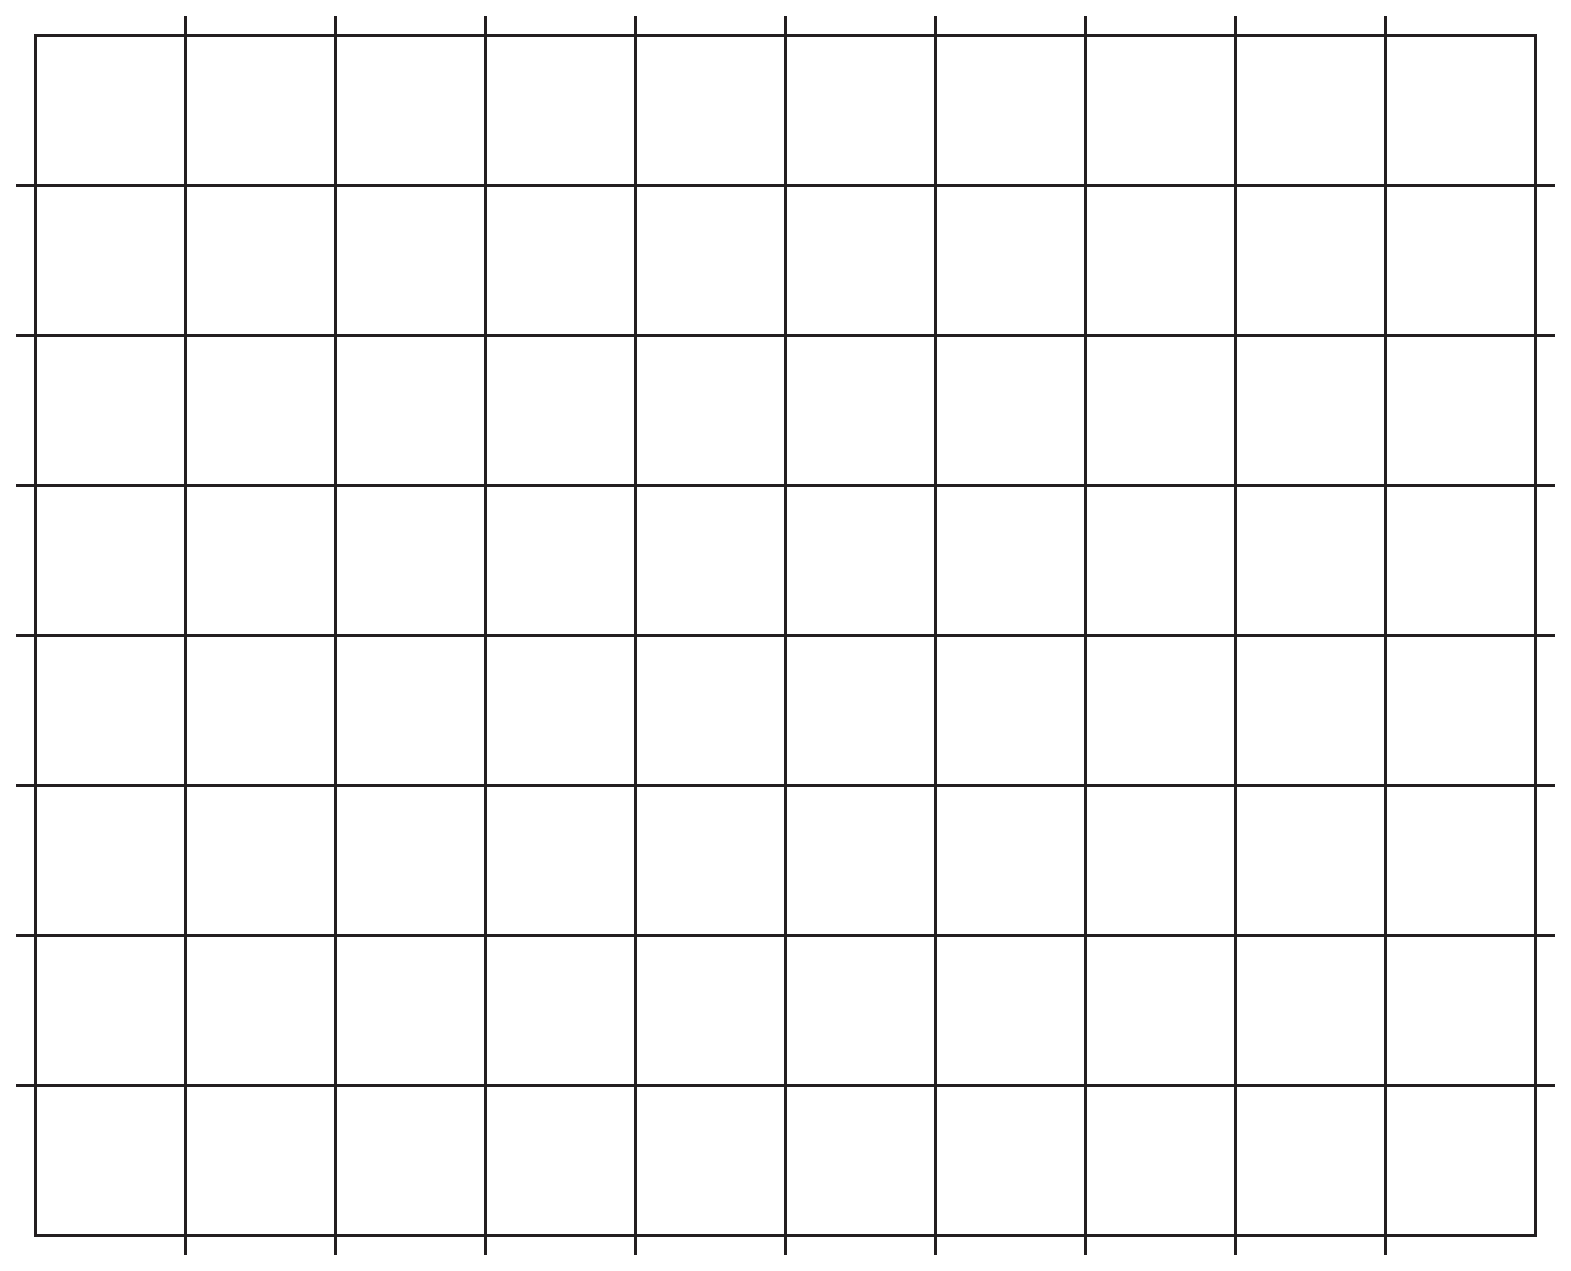
\includegraphics[keepaspectratio, scale=0.28, angle=0]
                  {figs/eps/grid.eps}
                  %\caption{オシロスコープの画面スケッチ}
                  \label{fig:grid50mV}
  \end{figure}

  \begin{spacing}{1.5}
  \begin{tabular}{|c||r|r|r|}
    \multicolumn{4}{c}{入力周波数 $f=800kHz\;$ の時の出力} \\ \hline
    項目 & DIVs & Value/DIV & Value \\ \hline \hline
    振幅pp &      & 500[mV]&      \\ \hline
    波長 &      & 500[ns]&      \\ \hline
  \end{tabular}
\end{spacing}
\end{multicols}

\newpage

\begin{figure}[H]
	\centering
	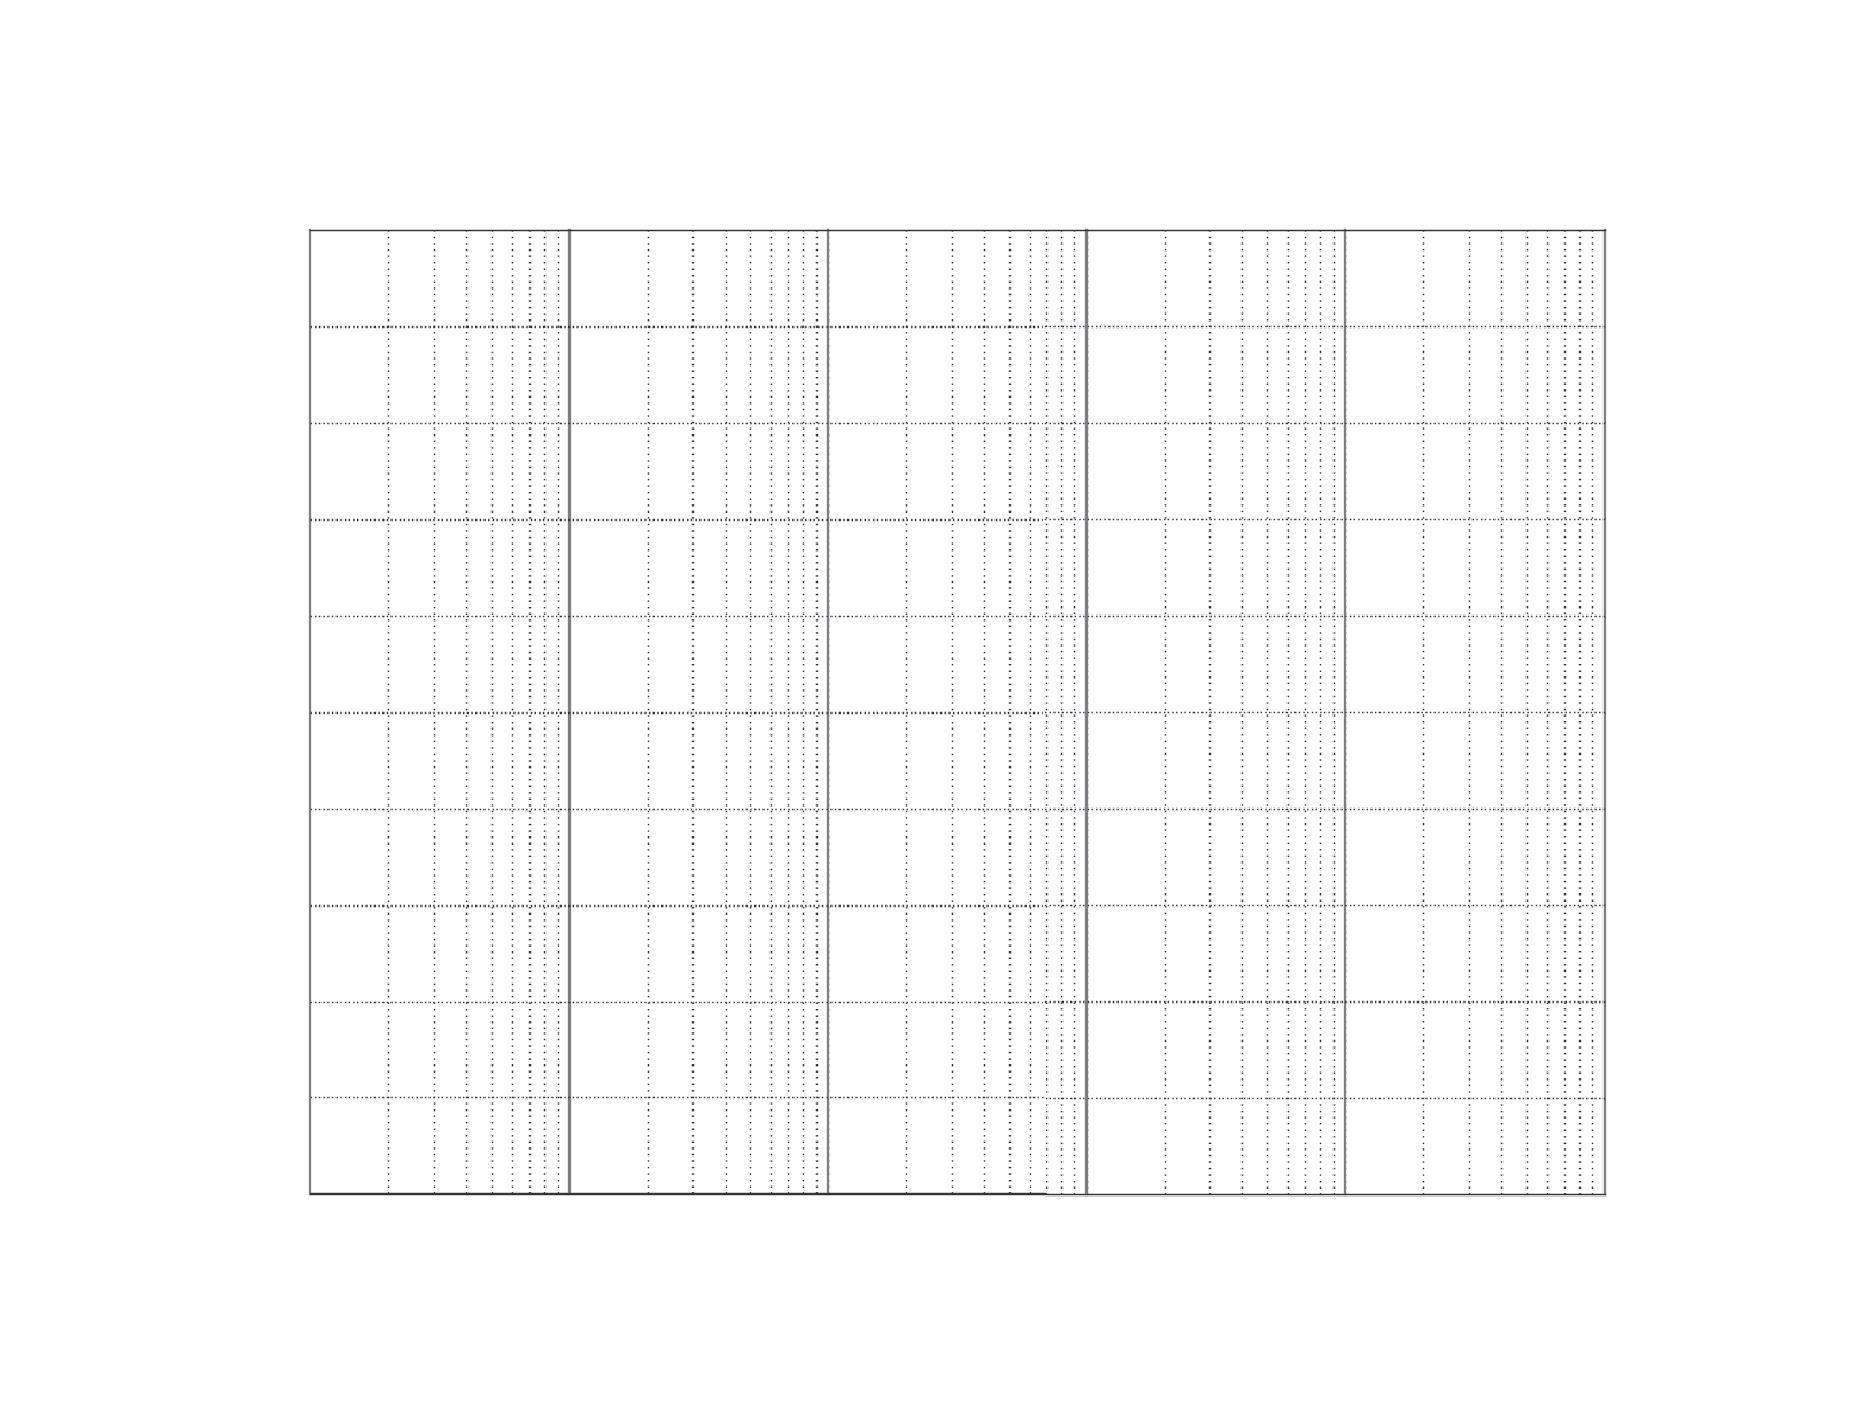
\includegraphics[keepaspectratio, scale=0.76, angle=90]
	{figs/eps/logscale.eps}
	\caption{周波数特性の片対数記録用紙}
	\label{fig:23}
\end{figure}

%\vfill

\end{document}